\listfiles
\documentclass[review]{elsarticle}

\usepackage{lineno,hyperref}
\modulolinenumbers[5]

\journal{Journal of \LaTeX\ Templates}

%%%%%%%%%%%%%%%%%%%%%%%
%% Elsevier bibliography styles
%%%%%%%%%%%%%%%%%%%%%%%
%% To change the style, put a % in front of the second line of the current style and
%% remove the % from the second line of the style you would like to use.
%%%%%%%%%%%%%%%%%%%%%%%

% Numbered
% \bibliographystyle{model1-num-names}

%% Numbered without titles
% \bibliographystyle{model1a-num-names}

%% Harvard
% \bibliographystyle{model2-names}\biboptions{authoryear}

%% Vancouver numbered
% \usepackage{numcompress}\bibliographystyle{model3-num-names}

%% Vancouver name/year
% \usepackage{numcompress}\bibliographystyle{model4-names}\biboptions{authoryear}

%% APA style
% \bibliographystyle{model5-names}\biboptions{authoryear}

%% AMA style
% \usepackage{numcompress}\bibliographystyle{model6-num-names}

\usepackage{graphicx}
\graphicspath{ {figures/} }

\usepackage{array}
\usepackage{multirow}




%% `Elsevier LaTeX' style, distributed in TeX Live 2019
\bibliographystyle{elsarticle-num}
% \usepackage{numcompress}\bibliographystyle{elsarticle-num-names}
% \bibliographystyle{elsarticle-harv}\biboptions{authoryear}
%%%%%%%%%%%%%%%%%%%%%%%

\begin{document}

\begin{frontmatter}

\title{Comparative Performance Evaluation of Hadoop on PaaS Proposals by Leveraging HiBench}

%\tnotetext[mytitlenote]{Fully documented templates are available in the elsarticle package on \href{http://www.ctan.org/tex-archive/macros/latex/contrib/elsarticle}{CTAN}.}

%% Group authors per affiliation:
\address[univ]{Bah\c{c}e\c{s}ehir \"{U}niversitesi, Be\c{s}ikta\c{s} - Istanbul, Turkey}
\address[emredpt]{School of Engineering, Big Data Analytics and Management}
\address[serkandpt]{Department of Software Engineering}

\author[univ,emredpt]{Uluer Emre \"{O}zdil\corref{correspondings}}
\ead{ulueremre@gmail.com}
\author[univ,serkandpt]{Serkan Ayvaz\corref{correspondings}}
\ead{serkan.ayvaz@eng.bau.edu.tr}

\cortext[correspondings]{Corresponding authors}


%\fntext[myfootnote]{Since 1880.}

%% or include affiliations in footnotes:
%\author[mymainaddress,mysecondaryaddress]{Elsevier Inc}
%\ead[url]{www.elsevier.com}

%\author[mysecondaryaddress]{Global Customer Service\corref{mycorrespondingauthor}}
%\cortext[mycorrespondingauthor]{Corresponding author}
%\ead{support@elsevier.com}

%\address[mymainaddress]{1600 John F Kennedy Boulevard, Philadelphia}
%\address[mysecondaryaddress]{360 Park Avenue South, New York}



\begin{abstract}
The advent of Big Data emerged in any data-driven domain and scaled up the extent as well as the depth of data and its handling. In an ongoing maturing process, new approaches leaning on enhanced distributed storage and computing paradigms are invented helping overcome management and running analytics challenges. In this context Hadoop is embraced in a wide scale by beneficiants both from industry and academia since its first release in 2005. The commercialization of Cloud Computing started a grand migration movement towards cloud, applying also for Hadoop transferring its presence from on-premises to virtual machines stored and tamed in large data center facilities by global Cloud Service Providers. The CSPs' response to result-focused analytics purposes emerged a service called managed systems where the hard workload of multi node cluster implementation is overtaken by the contractor providing a pre-configured Hadoop package simplifying the installation process to a matter of property selection thus eliminating technical know-how requirements on such an implementation. Converting the concept of cloud based Hadoop from IaaS to PaaS apparently reduced costs commercially presented as pay-as-you-go or pay-per-use. There is a payoff, though, managed Hadoop systems do present a black-box behavior to the end user who cannot be clear on the inner performance dynamics, hence the benefits by leveraging them. In this study we selected three global providers (GCP, Azure, and Alibaba Cloud), activated their Hadoop PaaS services (Dataproc, HDInsight, and e-MapReduce, respectively) within same geographical region and by promise apparently same computing specifications, and executed several Hadoop workloads of the HiBench Benchmark Suite. The results yield that apparently same computation specs among CSPs' services do not necessarily guarantee equal or close performance outputs to each other. Our assumption is that the pre-configuration work of managed systems done by the contractor play a weighing role on their performance.
\end{abstract}

\begin{keyword}
%%\texttt{elsarticle.cls}\sep \LaTeX\sep Elsevier \sep template
\texttt{elsarticle.cls}\sep Benchmark Hadoop PaaS\sep HiBench\sep Performance evaluation

\MSC[2010] 00-01\sep  99-00
\end{keyword}

\end{frontmatter}

\linenumbers

%%\section{The Elsevier article class}
\section{Introduction}

Big Data has become an indispensable aspect for enterprises and academia of the information era to deal with. As the global internet access rate covers a weighing majority of the global human population, mobile technology devices become democratized, sensors and IoT devices the more occupy daily life, ongoing scientific researches produce vast amounts of data outputs the Big Data phenomenon gathered itself by means of overwhelming size with Volume, ever accelerating growth rate with Velocity, and splitting into diverse structures with Variety, new approaches were forced to mature in order to ease the maintenance of Big Data and enable extracting valuable insights from it leveraging complex statistical formulae. Distributed frameworks for storage and computation sparked up first by search engines were inherited and furtherly developed by the open source community yielding what is known as Hadoop and its ecosystem today. Considering the complexity of dealing with big data Hadoop represents a modern analytics framework decreasing management efforts and duration of analytics operations to an acceptable level by means of affordable commodity computers.

In parallel, the commercialization of Cloud Computing in the early 2000's delivered utilization of storage and computing resources to the end users saving them high investments on hardware technology that is soon going to be obsolete and is expensive to maintain. As the migration to the cloud is an ongoing process, Hadoop also slips out from its residence on on-prem infrastructure to the cloud by being implemented on virtual machine instances provided as IaaS platforms by many providers. The Cloud Service Providers embraced the need of eliminating Hadoop's complex implementation process on multi-node VMs by providing managed Hadoop systems commercially packaged as PaaS, which are pre-installed and pre-configured Hadoop clusters allowing the installation of tens to hundreds of nodes in a matter of minutes by simply determining some settings like hardware specs and node numbers prior the installation. The Managed Hadoop system is both a blessing and a curse, by leaving the hard implementation part which is not necessarily related with the main analysis objective to a contractor the end user saves time and efforts including a payoff, though: By definition, managed systems are prepackaged solutions provided in black-box nature. CSP apply behind-the-scenes tweaks in terms of reaching better performance results on selected approaches like memory intensive or compute intensive applications.

In this study we put three CSP providers' managed Hadoop services in focus in terms of performance evaluation comparison: GCP Dataproc, Azure HDInsight, and Alibaba Cloud e-MapReduce, each recognized in Gartner's 2020 report in leading or niche section. Bound by availability of their offered hardware and software options we selected by providers' promise apparently same or close settings. Without any performance tweak operation with their settings for any performance optimization on the respective managed systems after installation we immediately executed several workloads from HiBench's micro, sql, ml, and websearch categories. For a more clear understanding of the benchmark outputs, during the benchmark execution we collected system utilization records on each worker node of the cluster. The results yield that Hadoop PaaS offerings by vendor's promise side perform and system utilizations may highly vary among CSPs.

\section{Related Work}
HiBench is a tool to measure a specific system’s performing behaviour during execution. The conceptualization of conducting a benchmark may arise from different soils. Based on the conductor’s motivation; a benchmark’s use case could be an inner evaluation of a system’s performance before and after some configuration tweaks are set, comparison of rival / complementary systems, or putting CSP’s cloud infrastructure services on scale. Following literature has been searched with finding different use cases of HiBench benchmarking suite in mind. 

Poggi et al. [52] Characterizing BigBench…

Poggi et al. the state of SQL on Hadoop [53]…

Samadi et al. conduct an experimental comparison between Spark and Hadoop installed on virtual machines on Amazon EC2 by leveraging nine among the provided HiBench workloads. Accuracy reasons led the conductors run the workloads three times concluding input data scales of 1, 3, and 5 GB respectively. Based on the outputs comprising duration, throughput, speed up, and CPU/memory consumption, the conclusion draws Spark consuming less CPU and performing better on all workload results over Hadoop. 

Ahn et al. [54] put Spark on YARN’s performance on test with HiBench in terms of handling a deluge of data generated by IoT devices. The experiment is run on a cluster with one master and 3 worker nodes each node possessing Intel® Xeon® processor with 20 cores and 128GB main memory meaning 60 cores and 384GB memory in total. HiBench’s workloads Micro (comprising Sort, TeraSort, and Wordcount), SQL (comprising Aggregation, Join, and Scan), and Machine Learning (comprising Bayes, Logistic Regression, Gradient Boosting Tree, Random Forest, and Linear Regression) are leveraged by a chosen data scale of 30 GB. Spark occupies memory during the whole job execution which in result reduces IOs’ negative impact on processor performance. For optimizing resource usage the conductors modified YARN’s minimum memory allocation and Spark executor settings so that the Spark executors’ overall loads remain below total system memory. Alongside with HiBench’s duration and throughput report, CPU / memory utilization and disk throughput are profiled as well. Finding of this paper points out that Spark guarantees performance when provided with enough memory.

Han et al. [55] study the impact of memory size on big data processing by means of Hadoop and Spark performance comparison leveraging HiBench’s k-Means workload as the only benchmark. For each of the specified memory sizes of 4, 8, and 12 GB, iterating through a data scale of 1 to 8 GB, with 1GB increment inbetween, k-Means benchmark for Hadoop and Spark is executed. The results depict Spark’s overperforming Hadoop unless the total input data size is smaller than 33.5\% of the total memory size assigned to worker nodes. After reaching that ratio Spark suffers with insufficient memory resources and is led to interoperate with HDFS causing a sharp decrease in its performance and brings Hadoop in throughput and duration performance to the front. The conductors make a second experiment to find out if Spark’s performance can be improved by tweaking the allocation setting for storage memory and shuffle memory while remaining within the specified memory limitations of 4, 8 and 12 GB. Executing HiBench’s k-means benchmark outputs a report interpreted by the conducters as Spark show a 5-10\%, and 15\% maximum improvement in processing time.

Ivanov et al. [56] compare the performances of two enterprise grade applications, DataStax Enterprise (DSE), a production level implementation of Apache Cassandra with extended features like in memory computing and advanced security to name but two, and Cloudera’s Distribution of Hadoop (CDH) comprising core Hadoop elements HDFS and YARN integrated with elements belonging to the Hadoop ecosystem. DSE’s HDFS compatible file system CSF lets Hadoop applications run without any modification. The conductors installed the latest stable releases of both softwares on equal CPU, memory and network infrastructure configuration. For both installations, default system parameters have been left with their defaults. HiBench’s three chosen workloads (CPU-bound wordcount, IO-bound dfsioe, and mixed HiveBench) are executed three times, the average values have been taken for representativeness. Several conclusions of their study proclaim linearly scaling of both systems by the increase of data size, while CDH outperforms DSE in read intensive workloads, DSE performs better in write intensive workloads. Leveraging HiBench is where this study differs in approach related to other studies using YCSB benchmark suite. HiBench’s results confirm the latter’s output as well.




\section{Method}
CSP configurations in Table \ref{tab:csp-configs}


\begin{table}
	\centering
	\small
	\caption{Selected configurations on CSPs’ managed Hadoop services}
	\label{tab:csp-configs}
	\begin{tabular}[h]{ p{2.5cm} p{2.5cm} p{3.7cm} p{3cm}  }
		\hline
		{} & \textbf{GCP} & \textbf{Azure} & \textbf{Alibaba Cloud}\\
		\hline
		Service & Dataproc & HDInsight & e-MapReduce \\
		Region & europe-west3-a & Germany West Central & eu-central-1 \\
		Location & Frankfurt & Frankfurt & Frankfurt \\
		Image & 1.4-ubuntu18  & HDI 3.6 & EMR-3.32.0 \\
		OS & ubuntu18.04 & ubuntu 16.04 & Aliyun Linux 2 \\
		Hadoop v. & 2.9 & 2.7.3 & 2.8.5 \\
		Java & 1.8.0\_275 & 1.8.0\_275 & 1.8.0\_252 \\
		\hline
		\multicolumn{4}{ c }{MASTER NODE} \\
		\hline
		Machine Type & e2-highmem-8 & A8m v2 & ecs.se1.2xlarge \\
		Processors & 8 vCPU & 8 cores & 8 vCPU \\
		Memory & 64 GB RAM & 64 GB RAM & 64 GB RAM \\
		\hline
		\multicolumn{4}{ c }{WORKER NODES} \\
		\hline
		\# Nodes & 3 & 3 & 3 \\
		Machine Type & e2-highmem-4 & A4m v2 & ecs.se1.xlarge \\
		Processors & 4 vCPU & 4 cores & 4 vCPU \\	
		Memory & 32 GB RAM & 32 GB RAM & 32 GB RAM \\	
		Storage & HDFS 1000 GB & \multirow{3}{ 8em }{WASB \\
			\textit{Azure blob storage}} & HDFS 1000 GB \\	
		Replication & 2 &  & 2 \\	
		Block size & 128 MB &  & 128 MB \\
		\hline
	\end{tabular}
\end{table}


\section{Results}
Table \ref{tab:uc1-results} and Table \ref{tab:uc2-results} summarize HiBench benchmark execution outputs.

%%Use Case 1 Tabular Results:
\begin{table}
	\centering
	\small
	\caption{Use Case 1 benchmark outputs}
	\label{tab:uc1-results}
	\begin{tabular}[h]{ r r r r r r r r }
		\multicolumn{4}{ l }{Data Scale: Huge} & & & & \\
		{} & {} & \multicolumn{2}{ c }{\textbf{Dataproc}} & \multicolumn{2}{ c }{\textbf{HDInsight}} & \multicolumn{2}{ c }{\textbf{e-MapReduce}} \\
		\hline
		{Benchmark} & {IDS} & \begin{math}D_{(s)}\end{math} & \begin{math}T_{(b/s)}\end{math} & \begin{math}D_{(s)}\end{math} & \begin{math}T_{(b/s)}\end{math} & \begin{math}D_{(s)}\end{math} & \begin{math}{T_{(b/s)}}\end{math} \\
		\hline
		Sort & 3.28 GB & 70 & 47110942 & 131 & 25076597 & 111 & 29419903 \\
		Terasort & 32.00 GB & 667 & 47988314 & 858 & 37277268 & 1054 & 30374710 \\
		Wordcount & 32.85 GB & 978 & 33594975 & 1470 & 22340906 & 889 & 36949719 \\
		Dfsioe-r & 26.99 GB & 294 & 91772636 & 662 & 40787869 & 245 & 110206431 \\
		Dfsioe-w & 27.16 GB & 379 & 71733304 & 658 & 41296567 & 281 & 96488258 \\
		Scan & 2.01 GB & 73 & 27629405 & 157 & 12830581 & 74 (*) & 27193804 (*) \\
		Join & 1.92 GB & 181 & 10614143 & 356 & 5390513 & 175 (*) & 10950553 (*) \\
		Aggregation & 372.38 MB & 97 & 3857328 & 215 & 1728400 & 97 (*) & 3849353 (*) \\
		Bayes & 1.88 GB & 2604 & 722498 & 6120 & 307708 & 3017 & 623692 \\
		Kmeans & 20.08 GB & 2321 & 8652662 & 2313 & 8683526 & 2070 & 9703348 \\
		Pagerank & 2.99 GB & 1544 & 1938541 & 3334 & 897807 & 2458 & 1217764 \\
		\hline
		\multicolumn{4}{ l }{Data Scale: Gigantic} & & & & \\
		{} & {} & \multicolumn{2}{ c }{\textbf{Dataproc}} & \multicolumn{2}{ c }{\textbf{HDInsight}} & \multicolumn{2}{ c }{\textbf{e-MapReduce}} \\
		\hline
		{Benchmark} & {IDS} & \begin{math}D_{(s)}\end{math} & \begin{math}T_{(b/s)}\end{math} & \begin{math}D_{(s)}\end{math} & \begin{math}T_{(b/s)}\end{math} & \begin{math}D_{(s)}\end{math} & \begin{math}{T_{(b/s)}}\end{math} \\
		\hline
		Sort & 32.85 GB & 715 & 45939699 & 787 & 41721261 & 896 & 36680251 \\
		Terasort & 320.00 GB & 9821 & 32582430 & ---(**) & ---(**) & 9660 & 33126513 \\
		Wordcount & 328.49 GB & 10131 & 32423997 & 13596 & 24159989 & 8671 & 37882290 \\
		Dfsioe-r & 216.03 GB & 915 & 236107099 & 1886 & 114538844 & 660 & 327294273 \\
		Dfsioe-w & 217.33 GB & 1347 & 161394226 & 1914 & 113574850 & 1060 & 205123746 \\
		Scan & 20.10 GB & 457 & 43964927 & 514 & 39085260 & 407 (*) & 49378781 (*) \\
		Join & 19.19 GB & 595 & 32268936 & 761 & 25240939 & 594 (*) & 32319846 (*) \\
		Aggregation & 3.69 GB & 523 & 7051835 & 594 & 6203608 & 565 (*) & 6523381 (*) \\
		Bayes & 3.77 GB & 5350 & 703332 & 12589 & 299143 & 6363 & 591341 \\
		Kmeans & 40.16 GB & 4541 & 8844971 & 4042 & 9935665 & 4034 & 9956003 \\
		Pagerank & 19.93 GB & 8371 & 2381276 & 11779 & 1692241 & 13893 & 1434711 \\
		\hline
		\multicolumn{8}{ r }{(*) Benchmark execution succeeds after modifying preconfiguration, more on this in Discussion } \\
		\multicolumn{8}{ r }{(**) System failure due to insufficient space on HDFS, more on this in Discussion } \\
		\hline
		
		
	\end{tabular}
\end{table}



%% Use Case 2 Tabular Results:
\begin{table}
	\centering
	\small
	\caption{Use Case 2 benchmark outputs}
	\label{tab:uc2-results}
	\begin{tabular}[h]{ l r r r r r r r }
		%%\multicolumn{4}{ l }{Data Scale: Tiny} & & & & \\
		{} & {} & \multicolumn{2}{ c }{\textbf{Dataproc}} & \multicolumn{2}{ c }{\textbf{HDInsight}} & \multicolumn{2}{ c }{\textbf{e-MapReduce}} \\
		\hline
		{Benchmark} & {IDS} & \begin{math}D_{(s)}\end{math} & \begin{math}T_{(b/s)}\end{math} & \begin{math}D_{(s)}\end{math} & \begin{math}T_{(b/s)}\end{math} & \begin{math}D_{(s)}\end{math} & \begin{math}{T_{(b/s)}}\end{math} \\
		\hline
		Sort (t) & 39.30 KB & 36 & 1077 & 69 & 563 & 32 & 1173 \\
		Wordcount(t) & 38.65 KB & 38 & 1005 & 68 & 551 & 31 & 1242 \\
		%%\hline
		%%\multicolumn{4}{ l }{Data Scale: Small} & & & & \\
		%%{} & {} & \multicolumn{2}{ c }{\textbf{Dataproc}} & \multicolumn{2}{ c }{\textbf{HDInsight}} & \multicolumn{2}{ c }{\textbf{e-MapReduce}} \\
		%%\hline
		%%{Benchmark} & {IDS} & \begin{math}D_{(s)}\end{math} & \begin{math}T_{(b/s)}\end{math} & \begin{math}D_{(s)}\end{math} & \begin{math}T_{(b/s)}\end{math} & \begin{math}D_{(s)}\end{math} & \begin{math}{T_{(b/s)}}\end{math} \\
		%%\hline
		Sort (s) & 3.28 MB & 36 & 90155 & 70 & 47090 & 31 & 104865 \\
		Wordcount (s) & 348.29 MB & 50 & 6508975 & 98 & 3337158 & 47 & 7055759 \\
		%%\hline
		%%\multicolumn{4}{ l }{Data Scale: Large} & & & & \\
		%%{} & {} & \multicolumn{2}{ c }{\textbf{Dataproc}} & \multicolumn{2}{ c }{\textbf{HDInsight}} & \multicolumn{2}{ c }{\textbf{e-MapReduce}} \\
		%%\hline
		%%{Benchmark} & {IDS} & \begin{math}D_{(s)}\end{math} & \begin{math}T_{(b/s)}\end{math} & \begin{math}D_{(s)}\end{math} & \begin{math}T_{(b/s)}\end{math} & \begin{math}D_{(s)}\end{math} & \begin{math}{T_{(b/s)}}\end{math} \\
		%%\hline
		Sort (l) & 328.50 MB & 42 & 7860401 & 81 & 4065391 & 42 & 7741448 \\
		Wordcount (l) & 3.28 GB & 129 & 25448586 & 269 & 12195273 & 120 & 27269866 \\
		%%\hline
		%%\multicolumn{4}{ l }{Data Scale: Huge} & & & & \\
		%%{} & {} & \multicolumn{2}{ c }{\textbf{Dataproc}} & \multicolumn{2}{ c }{\textbf{HDInsight}} & \multicolumn{2}{ c }{\textbf{e-MapReduce}} \\
		%%\hline
		%%{Benchmark} & {IDS} & \begin{math}D_{(s)}\end{math} & \begin{math}T_{(b/s)}\end{math} & \begin{math}D_{(s)}\end{math} & \begin{math}T_{(b/s)}\end{math} & \begin{math}D_{(s)}\end{math} & \begin{math}{T_{(b/s)}}\end{math} \\
		%%\hline
		Sort (h) & 3.28 GB & 70 & 47077081 & 141 & 23355371 & 107 & 30693426 \\
		Wordcount (h) & 32.85 GB & 952 & 34512554 & 1487 & 22093900 & 888 & 36991074 \\
		%%\hline
		%%\multicolumn{4}{ l }{Data Scale: Gigantic} & & & & \\
		%%{} & {} & \multicolumn{2}{ c }{\textbf{Dataproc}} & \multicolumn{2}{ c }{\textbf{HDInsight}} & \multicolumn{2}{ c }{\textbf{e-MapReduce}} \\
		%%\hline
		%%{Benchmark} & {IDS} & \begin{math}D_{(s)}\end{math} & \begin{math}T_{(b/s)}\end{math} & \begin{math}D_{(s)}\end{math} & \begin{math}T_{(b/s)}\end{math} & \begin{math}D_{(s)}\end{math} & \begin{math}{T_{(b/s)}}\end{math} \\
		%%\hline
		Sort (g) & 32.85 GB & 694 & 47300549 & 699 & 47000056 & 883 & 37192377 \\
		Wordcount (g) & 328.49 GB & 9749 & 33696143 & 13286 & 24725537 & 8622 & 38100208 \\
		\hline
		\multicolumn{8}{ r }{(t): tiny, (s): small, (l): large, (h): huge, (g): gigantic} \\
		\hline
	\end{tabular}
\end{table}



%%Use Case 1 Comparative Results:
\begin{table}
	\centering
	\small
	\caption{Use Case 1 Comparative benchmark outputs}
	\label{tab:uc1-comparative-results}
	\begin{tabular}[h]{ r r r r r r r r }
		\multicolumn{6}{ l }{Data Scale: Huge}  \\
		{Benchmark} & First & Second & -Perf.\% & Third & -Perf.\% \\
		\hline
		Sort & GCP & Alibaba & -58.57\% & Azure & -87.14\% \\
		Terasort & GCP & Azure & -28.64\% & Alibaba & -58.02\% \\
		Wordcount & Alibaba & GCP & -10.01\% & Azure & -65.35\% \\
		Dfsioe-r & Alibaba & GCP & -20.00\% & Azure & -170.20\% \\
		Dfsioe-w & Alibaba & GCP & -34.88\% & Azure & -134.16\% \\
		Scan & GCP & Alibaba & -1.37\% & Azure & -115.07\% \\
		Join & Alibaba & GCP & -3.43\% & Azure & -103.43\% \\
		Aggregation & GCP-Alibaba & --- & --- & Azure & -121.65\% \\
		Bayes & GCP & Alibaba & -15.86\% & Azure & -135.02\% \\
		Kmeans & Alibaba & Azure & -11.74\% & GCP & -12.13\% \\
		Pagerank & GCP & Alibaba & -59.20\% & Azure & -115.93\% \\
		\hline
		\multicolumn{6}{ l }{Data Scale: Gigantic}  \\
		{Benchmark} & First & Second & -Perf.\% & Third & -Perf.\% \\
		\hline
		Sort & GCP & Azure & -10.07\% & Alibaba & -25.31\% \\
		Terasort & Alibaba & GCP & -1.67\% & Azure & --- \\
		Wordcount & Alibaba & GCP & -16.84\% & Azure & -56.80\% \\
		Dfsioe-r & Alibaba & GCP & -38.64\% & Azure & -185.76\% \\
		Dfsioe-w & Alibaba & GCP & -27.08\% & Azure & -80.57\% \\
		Scan & Alibaba & GCP & -12.29\% & Azure & -26.29\% \\
		Join & Alibaba & GCP & -0.17\% & Azure & -28.11\% \\
		Aggregation & GCP & Alibaba & -8.03\% & Azure & -13.58\% \\
		Bayes & GCP & Alibaba & -18.93\% & Azure & -135.31\% \\
		Kmeans & Alibaba & Azure & -0.20\% & GCP & -12.57\% \\
		Pagerank & GCP & Azure & -40.71\% & Alibaba & -65.97\% \\
		\hline
	\end{tabular}
\end{table}



\paragraph{Analysis}HiBench's Hadoop related benchmarks in groups micro (Sort, Terasort, Dfsioe, and Wordcount), sql (Scan, Join, and Aggregation), ml (Bayes and Kmeans), and websearch (Pagerank) have been executed on all three CSPs managed Hadoop services. During benchmark runtime resource utilization on worker nodes have been captured. The resulting multiplots are suggested to be read as follows: Top-left, top-right, and bottom-left plots represent CPU (user\%), Memory, and IO utilization on each worker node of the respective cluster over time. CPU utilization lines are given in blue tones, Memory utilization lines are given in fuchsia tones, IO-read and IO-write tps' are represented with orange tones and green tones, respectively. Even though the coloring convention might sound confusing, it gives a clear overview in terms of resource utilization of the total benchmark process over time. The left hand side x-axis measures CPU/Memory usage in percent, the right hand side x-axis measures IO-read or IO-write transfers in byte per second. The bottom-right plot represents the comparative benchmark performance outputs of the respective CSP. Duration measure in seconds is expected to perceived as "lower is better" while Throughput which is the amount of processed data per second in bytes is expected to perceived as "higher is better".





USE CASE 1: 
\paragraph{Sort - Huge} Figure \ref{fig:uc1-srt-h-cmidt}; CPU utilization in GCP and Alibaba condence around 80\% to 98\% whereas in Azure the range widens up between 50\% to 90\%. Memory loads in GCP and Alibaba among the worker nodes display a harmonic behavior between 20\% to 40\% and 90\% to 100\% respectively, whereas the memory load in Azure's worker nodes vary between 10\% and 50\%. In the second half of the benchmark execution IO write transfers in GCP and Alibaba show peaks at about 500 tps where in Azure it is limited with 100 tps. Resulting in GCP carrying out the highest Throughput, thus reaching the shortest Duration of 70 seconds.

\paragraph{Sort - Gigantic} Figure \ref{fig:uc1-srt-g-cmidt}; switching the data scale for Sort benchmark to gigantic, GCP's processor load condences around 80\% - 95\% where its memory load rises to range 80\% - 100\%; IO write transfers behave at about 500 tps where IO reads reach 1000 tps in the second half of the benchmark process. Azure's processor and memory performances depict a looser behavior not utilizing the maximum potential whereas IO-read and IO-write tps' reach their maximum at 200 and 350, respectively. Alibaba's resource utilization depicts a high memory load of 90\% - 100\% dropping to 70\% and about 83\% on partial nodes in the second half. As so with the processor load behaving between 80\% and 100\% in the first half dropping to about 50\% in the second half where IO write reaches peak at 800 tps. Resulting in GCP embarking highest and Azure the second highest Throughput, respective Durations output in 715 and 758 seconds.

\paragraph{Terasort - Huge} Figure \ref{fig:uc1-tera-h-cmidt}; GCP depicts a high utilization on processors at a range of 80\% - 100\%, memory moving from 80\% to 100\%, and IO behavior 500 tps in overall and peaking at 1000 tps in IO-read resulting in highest Throughput in 667 seconds response time among other CSPs. Azure's processor and memory utilization fluctuate in overall where memory performance incrementally reach 100\% in one node, a stable IO-write in overall process at about 70 tps peaking at 250 tps reaches the second highest Throughput in 858 seconds. Alibaba with high memory and processor utilization, and varying IO tps's in overall process falls back in embarking Throughput and resulting in 1054 seconds response time.

\paragraph{Terasort - Gigantic} Figure \ref{fig:uc1-tera-g-cmidt}; switching the scale to gigantic causes dramatic changes on resource utilization on all CSPs. During all benchmark process GCP depicts very condensed high utilization on processor at a broad range of 30\% to about 95\%, memory consumption between 95\% and 100\% and IO read transfer varying between 800 to 1100 tps. Azure on the other side, fails to complete the benchmark on 3 attempts; suffering from YARN insufficient HDFS allocation requested for bringing the job further. IO scores drop to null and task raises failure. Alibaba Cloud's resource utilization goes within maximum levels where processor utilization depicts a consumption of 80\% to 90\% in the overall, memory utilization at it highest during all process, IO reads and writes moving along the 600 tps' and peaking around 1600 tps. With a slicely higher value in Throughput, Alibaba performs best with 9660 seconds, followed by GCP with 9821 seconds. Azure disqualifies this session.

\paragraph{Wordcount - Huge} Figure \ref{fig:uc1-wrdcnt-h-cmidt}; GCP performing processor utilization of 75\% to 100\% with a memory consumption between 80\% to 95\% where IO transfers move along 60 tps peaking at about 150 tps reaches second highest Throughput with 978 seconds response time. Azure's processor utilization moving along 70\% to about 100\% where memory depicts 30\% to 50\% utilization and lower IO transfers peaking at about 60 tps reaches the lowest throughput hance the longest duration of 1470 seconds. Alibaba depicting high processor and memory load moving in ranges 70\% to 100\% and 80\% to slightly over 90\% with IO transfers moving along 200 tps peaking at 300tps to 350tps reaches the highest Throughput hence shortest execution time of 889 seconds.

\paragraph{Wordcount - Gigantic} Figure \ref{fig:uc1-wrdcnt-g-cmidt}; GCP utilizing processor and memory sources at their maximum during the overall process, for CPU within 60\% up to pushing 100\%, memory utilization varying between 60\% to 100\%, and IO-read and IO-write transfers moving along 90 tps and 250 tps respectively, reaches second highest Throughput load resulting in 10131 seconds response time. Azure shows a dens processor utilization varyimg between 40\%s and close to 100\%s, memory consumption is somehow oppressed to stay within range 20\% up to 50\%, IO behavior reacts seldomly over 60 tps resulting in the lowest Throughput and longest Duration of 13596 seconds. Alibaba depicting a high processor utilization within range 85\%-100\%, a relatively more stable memory consumption in range 85\% to 100\% and IO transfers mostly about 300 tps thus performing highest Throughput hence shortest response time of 8671 seconds.

\paragraph{Dfsioe-read - Huge} Figure \ref{fig:uc1-dfsioer-h-cmidt}; GCP's processor utilization moving roughly between 80\% to 95\% accompanied by memory utilization  within range slightly below and over 70\%, IO transfers peaking at 400 tps mostly go along 100 tps and 250 tps performs second highest Throughput resulting in 294 seconds of Duration. Azure's processor utilization is rather limited to between 60\% and 90\%whereas the memory utilization behaves between 10\% to 50\%, generally low IO transfers with two markable IO-read and IO-write condences reaching peaks at 2000 tps and 1500 tps respectively results in the lowest Throughput and 662 seconds of response time. Alibaba with 245 seconds Duration displays a similar resoure utilization pattern with GCP where it differentiates in memory utilization moving around 90\%s.

\paragraph{Dfsioe-read - Gigantic} Figure \ref{fig:uc1-dfsioer-g-cmidt}; processor utilization in GCP cloud concentrates within range of 80\% to 90\%, memory utilization moves around 95\% to 100\% whereas IO read transfers moving along about 500 tps brings its performance to second highest Throughput with 915 seconds Duration. Azure displays a performance within a range of 55\% up to 90\% in CPU utilization, 20\% to 55\% in memory utilization, and IO-write activity moving along 70 tps, IO-read showing peak at about 470 tps reaching the lowest performance in Throughput outputting 1886 seconds response time.
Alibaba system utilization moves along 80\%-90\% range for processing performance, 90\%-100\% for memory load and a behavior up to 1700 tps IO-write placing its performance to the highest Throughput with 660 seconds duration.

\paragraph{Dfsioe-write - Huge} Figure \ref{fig:uc1-dfsioew-h-cmidt}; in GCP processor utilization moves between 70\% and 90\%, memory load increments from 20\% up to 70\% whereas IO-write transfers move along 500 tps resulting in second shortest response time 379 seconds. Azure's CPU utilization around 60\% to 90\%, memory load moves between 20\% and 40\% whereas IO-write transfers vary about 20 tps to 80 tp peaking at about 120 tps by a Duration output of 658 seconds. Alibaba with processor utilization 80\% and 95\%, incrementing memory load from about 40\% up to 90\%-100\%, and IO-write transfers at about 100 tps to 600 tps peaking at about 800 tps performs the heaviest Throughput thus reaching the shortest response time with 281 seconds.

\paragraph{Dfsioe-write - Gigantic} Figure \ref{fig:uc1-dfsioew-g-cmidt}; GCP processor utilization moves along a broad range hitting up to 90\% load, memory load quickly rises to 95\%-100\% range and keeps its position in overall execution,  IO-writes move alond 500 tps to 600 tps placing GCP to the second best performance with 1347 seconds response time. Azure shows a CPU utization in a range 60\% up to 90\% until it drops to about 25\% in the 2/3th of the overall process, memory load moves along lower 20\% to upper 50\% until its sudden drop to upper 15\% simultaneously with CPU utilization where IO-write transfers peak at about 120 tps resulting in 1914 seconds response time. Alibaba performing the shortest response time with 1060 seconds displays a similar memory and processor utilization behaviour with GCP where it differs in IO-write transfers peaking at about 900 tps.

\paragraph{Scan - Huge} Figure \ref{fig:uc1-scan-h-cmidt}; GCP processor utilization condences between about 80\% and 90\% during benchmark execution, memory load depicts movement between 20\% and 40\% accompanied by an IO-write transfer reaching over 500 tps which brings GCP to the leading performance within this benchmark with 73 seconds. On Azure's side processor utilization moves along 80\%-90\% range whereas memory load increments from the 15\%s to the 30\%s, relatively low IO-write tansfer peaking at about 85 tps results in lowest Throughput and 157 seconds Duration. Alibaba follows a similar pattern like GCP in resource utilization with about 90\% CPU load, 15\% to below 40\% memory utilization but a less dense IO-write transfer peaking at about 550 tps and so reaching a close Throughput to GCP resulting in 74 seconds response time.

\paragraph{Scan - Gigantic} Figure \ref{fig:uc1-scan-g-cmidt}; GCP's CPU utilization varying between 50\%s and 90\%s with a convergence at about 80\%s, memory load showing similar range with utilization reaching up 100\%s and IO-write transfers moving between 500 tps and 600 tps results in second highest Throughput by a 457 seconds response time. Azure's CPU utilization condences between 80\% and 90\% and memory load incrementing two times from 20\%s to 40\%s, IO-write transfer moving along 50 tps to 60 tps peaking at about 200 tps results in 514 seconds Duration. Alibaba's processor utilization moves in a relatively higher range between 80\% and 95\%, an incrementing memory load range from 40\%s-50\%s to 80\%s-100\%s during runtime, and IO-write transfers peaking at about over 500 tps results in highest Throughput thus shortest Duration of 407 seconds.

\paragraph{Join - Huge} Figure \ref{fig:uc1-join-h-cmidt}; GCP processor load moves mainly between 80\%s and over 90\%s, memory utilization moves along about 20\%s and 30\%s, IO-writes behaving at about 150 tps brings outputs 181 seconds response time. Azures resource utilization shows range between 80\% and 90\% for CPU, varying memory loads moving along below 20\%s and below 60\%s, IO-write transfers behave below 60 tps with a peak of 100 tps resulting in a lower throughput and response time of 356 seconds. Resource utilization at Alibaba behaves similar to GCP in processor and memory load whereas IO-write peaks at about 260 tps, reaching highest Throughput and a Duration of 175 seconds.

\paragraph{Join - Gigantic} Figure \ref{fig:uc1-join-g-cmidt}; CPU load in GCP moves along 70\% to 90\% in overall whereas RAM utilization among worker nodes takes a path within 50\% to 90\% range, IO-write transfers observed in behaviour about 100 tps resulting in a Throughput outputting 595 seconds of response time. Azure's resource utilization dynamics show a utilization of 80\% to 90\% with decreasing utilization on some worker nodes in later stage, memory utilization moving along the range 20\% up to 60\% and IO-write transfer observations peaking at 120 tps provide the lowest Throughput hence the longest response time of 761 seconds. Alibaba performing a processor utilization of about below 90\% to below 100\%, memory load behavior moving along 50\% to below 70\%, and IO-write observation peaking at 350 tps performans a slightly higher Throughput than GCP hence slightly shorter Duration of 594 seconds.

\paragraph{Aggregation - Huge} Figure \ref{fig:uc1-aggreg-h-cmidt}; GCP processor utilization moving around 80\% to about 95\%, memory load behaving between 15\% to 40\%, and IO-write transfer observed at about 150 tps results in 97 seconds Duration. Azure's CPU utilization behaves between 80\% and 90\% whereas memory load moves along from 10\% to varying utilizations among worker nodes up to 30\% and below 60\%, and IO-write transfers peaking at about 180 tps performs a relatively small Throughput resulting in 215 seconds completion time. Alibaba resource utilization moving along between 80\% and 90\% for CPU, 10\% to 40\% in memort, and IO-write transfer average of 26 tps show close performance to GCP resulting in same completion time of 97 seconds.

\paragraph{Aggregation - Gigantic} Figure \ref{fig:uc1-aggreg-g-cmidt}; processor utilization moving between 80\% and 90\% in overall execution, memory load between 50\% and 70\% peaking to below 100\%, IO-write transfers reaching a dense behavior at the end reaching 500 tps results in highest Throughput and 523 seconds response time. Azure displays a CPU utilization of below 80\% to above 90\%, mild RAM utilization moving along 30\%s to 60\%s, IO-write transfers behaving about 100 tps result in a relative low Throughput and 594 seconds of Duration to complete. Alibaba's processor load moves along 80\% to below 100\%, IO-write transfer behavior scaling from about 50 tps to 400 tps results in 565 seconds response time.	

\paragraph{Bayes - Huge} Figure \ref{fig:uc1-bayes-h-cmidt}; GCP in processor behavior moving along about 70\%s to below 100\%, memory load at about 30\% with a short peak to below 100\% at te first half, an IO-write transfer behavior about 500 tps resulting in highest Throughput thus fastest response time of 2604 seconds. Azure showing a splitted bevahior in CPU utilization among worker nodes where one load moves along about 80\% to lower 100\% and one node depicst a movement along minimum to about 20\%, memory loads also varying from each other by about 20\% load difference at the beginning however meeting the similar range starting at the second half, IO observations depict a low range with exception at the high IO-write transfer at about 3200 tps at the initial state of the execution result in a relatively low Throughput hence longest Duration of 6120 seconds. Alibaba CPU utilization shows varieties among worker nodes in load ranges, RAM utilization condences at higher levels ove 80\%, IO trransfers moving along 100tps to observable 450 tps resulting in 3017 seconds response time.

\paragraph{Bayes - Gigantic} Figure \ref{fig:uc1-bayes-g-cmidt}; GCP's processor utilization moving along 70\% to below 100\%, accompanied by memory load incrementing from 40\%s to 70\%s becoming stable at 50\%s, and IO-write transfers moving along 500 tps results in the highest Throughput and 5350 seconds of response time. Azure's resource utilization shows distinction in CPU and memory among worker nodes while two nodes depict higher utilization at about 70\% to below 100\% for processing and 40\%-50\% for memory, one node staying at lower levels for respective resources, the observed IO-write transfer move along 100 tps where IO-read transfer peaks at about 650 tps resulting in a lowest performance of 12589 seconds Duration. Alibaba depicting different utilization ranges among worker nodes for processing, the memory consumption follows a more balanced load among worker nodes with IO-write transfer  moving aong 200 tps a relatively lower Throughput hence relatively longer Duration of 6363 seconds, with respect to GCP.

\paragraph{Kmeans - Huge} Figure \ref{fig:uc1-kmeans-h-cmidt};

\paragraph{Kmeans - Gigantic} Figure \ref{fig:uc1-kmeans-g-cmidt};

\paragraph{Pagerank - Huge} Figure \ref{fig:uc1-page-h-cmidt};

\paragraph{Pagerank - Gigantic} Figure \ref{fig:uc1-page-g-cmidt};


\begin{figure}[b]
	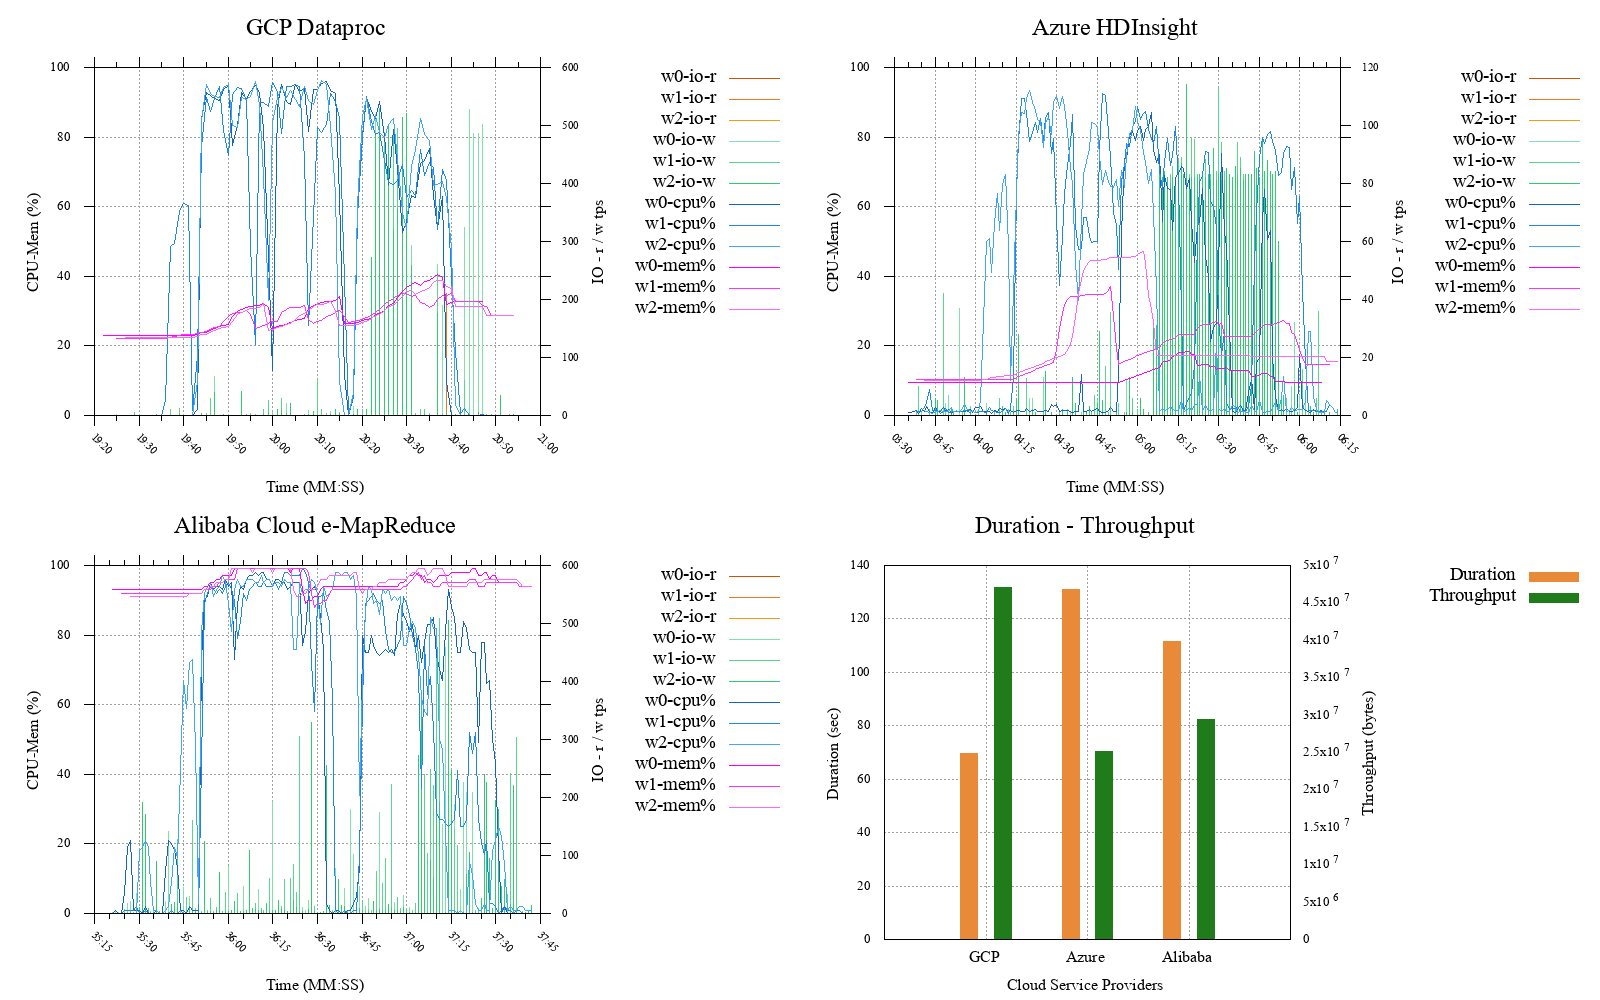
\includegraphics[width=\textwidth]{uc1-srt-h-cmidt}
	\caption{UC1 - Sort (Huge; 3.2 GB)}
	\label{fig:uc1-srt-h-cmidt}
	\centering
\end{figure}

\begin{figure}[b]
	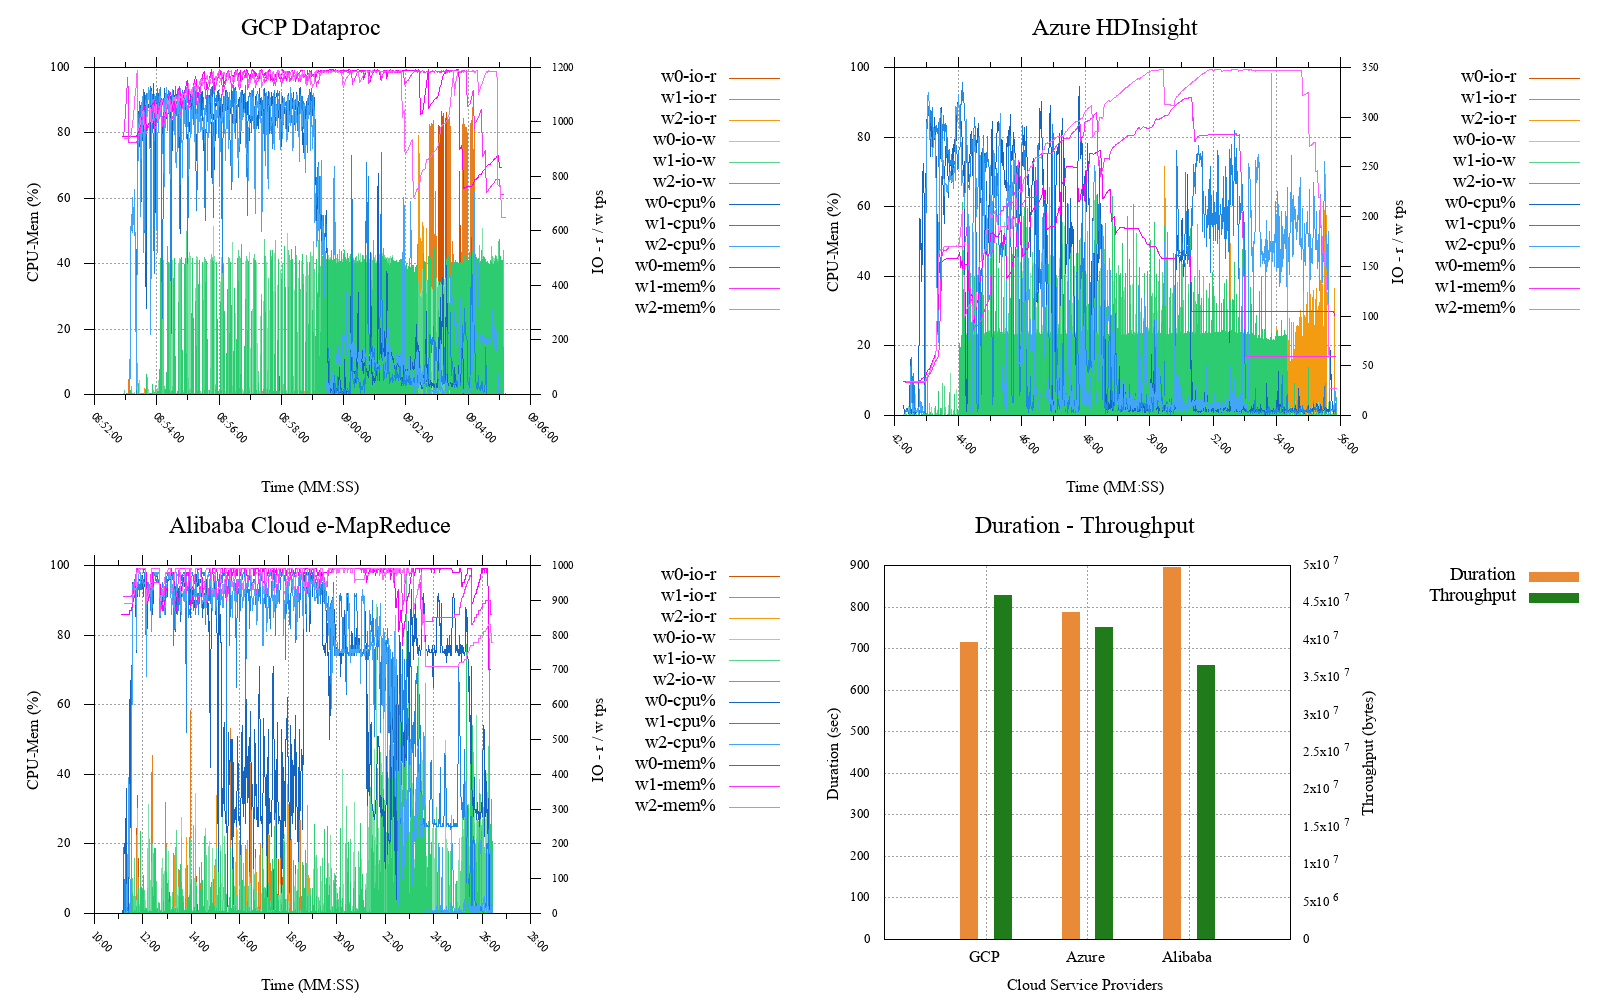
\includegraphics[width=\textwidth]{uc1-srt-g-cmidt}
	\caption{UC1 - Sort (Gigantic; 32 GB)}
	\label{fig:uc1-srt-g-cmidt}
	\centering
\end{figure}

\begin{figure}[b]
	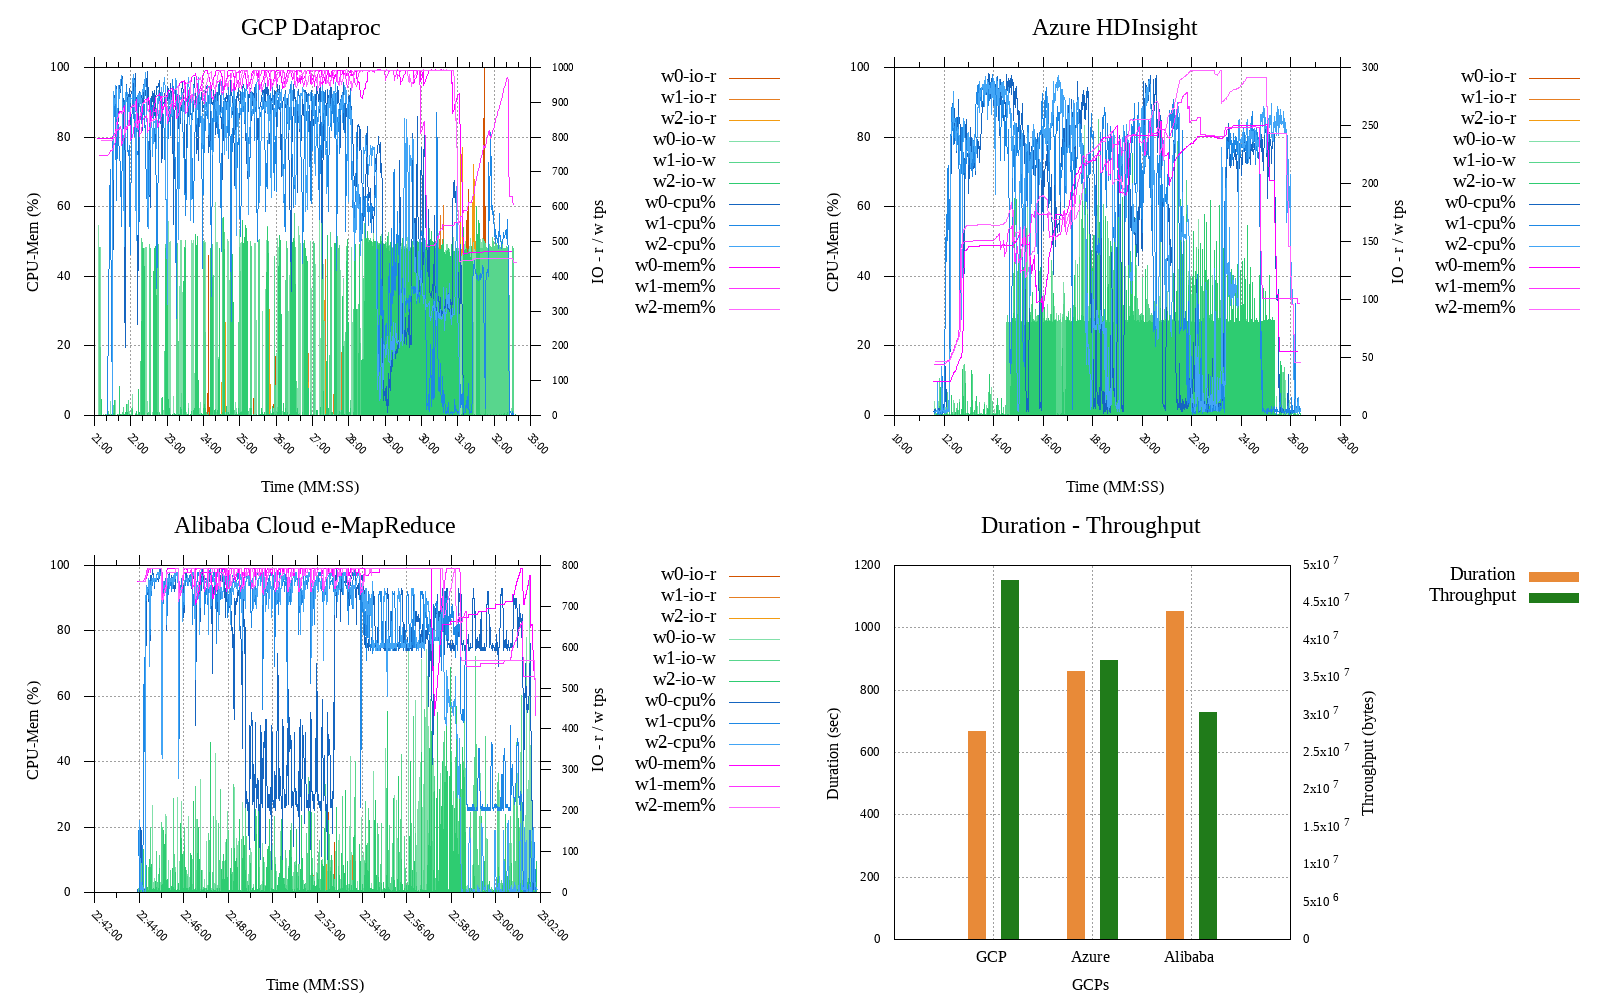
\includegraphics[width=\textwidth]{uc1-tera-h-cmidt}
	\caption{UC1 - Terasort (Huge; 320 MB)}
	\label{fig:uc1-tera-h-cmidt}
	\centering
\end{figure}

\begin{figure}[b]
	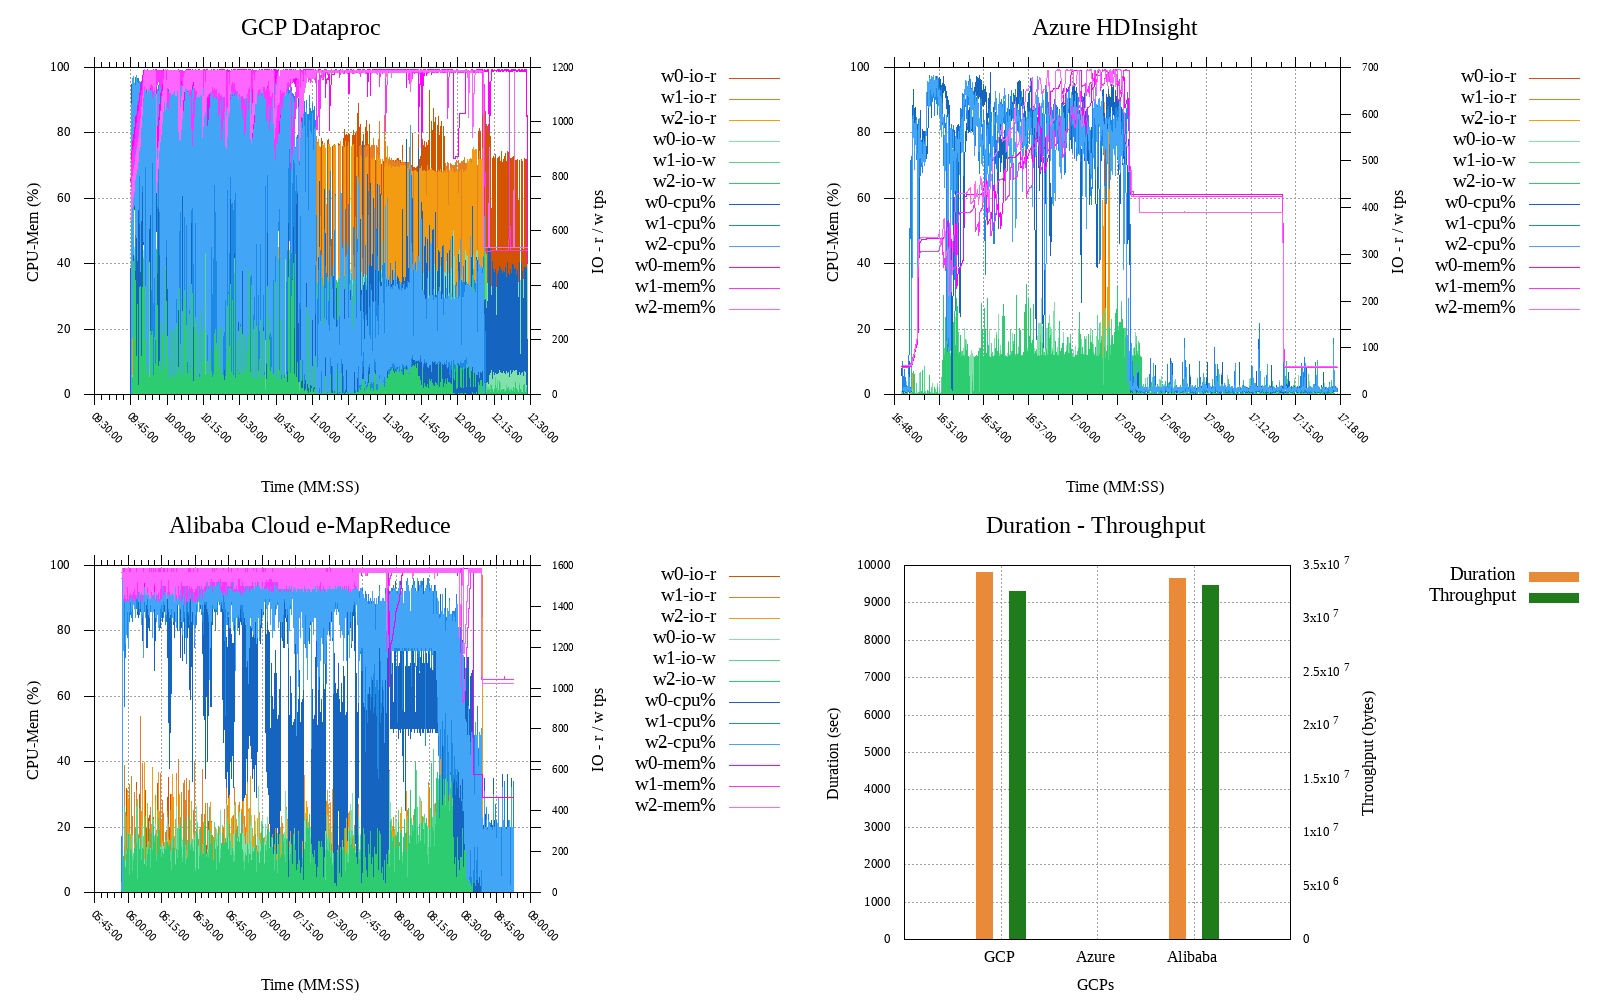
\includegraphics[width=\textwidth]{uc1-tera-g-cmidt}
	\caption{UC1 - Terasort (Gigantic; 3.2 GB)}
	\label{fig:uc1-tera-g-cmidt}
	\centering
\end{figure}

\begin{figure}[b]
	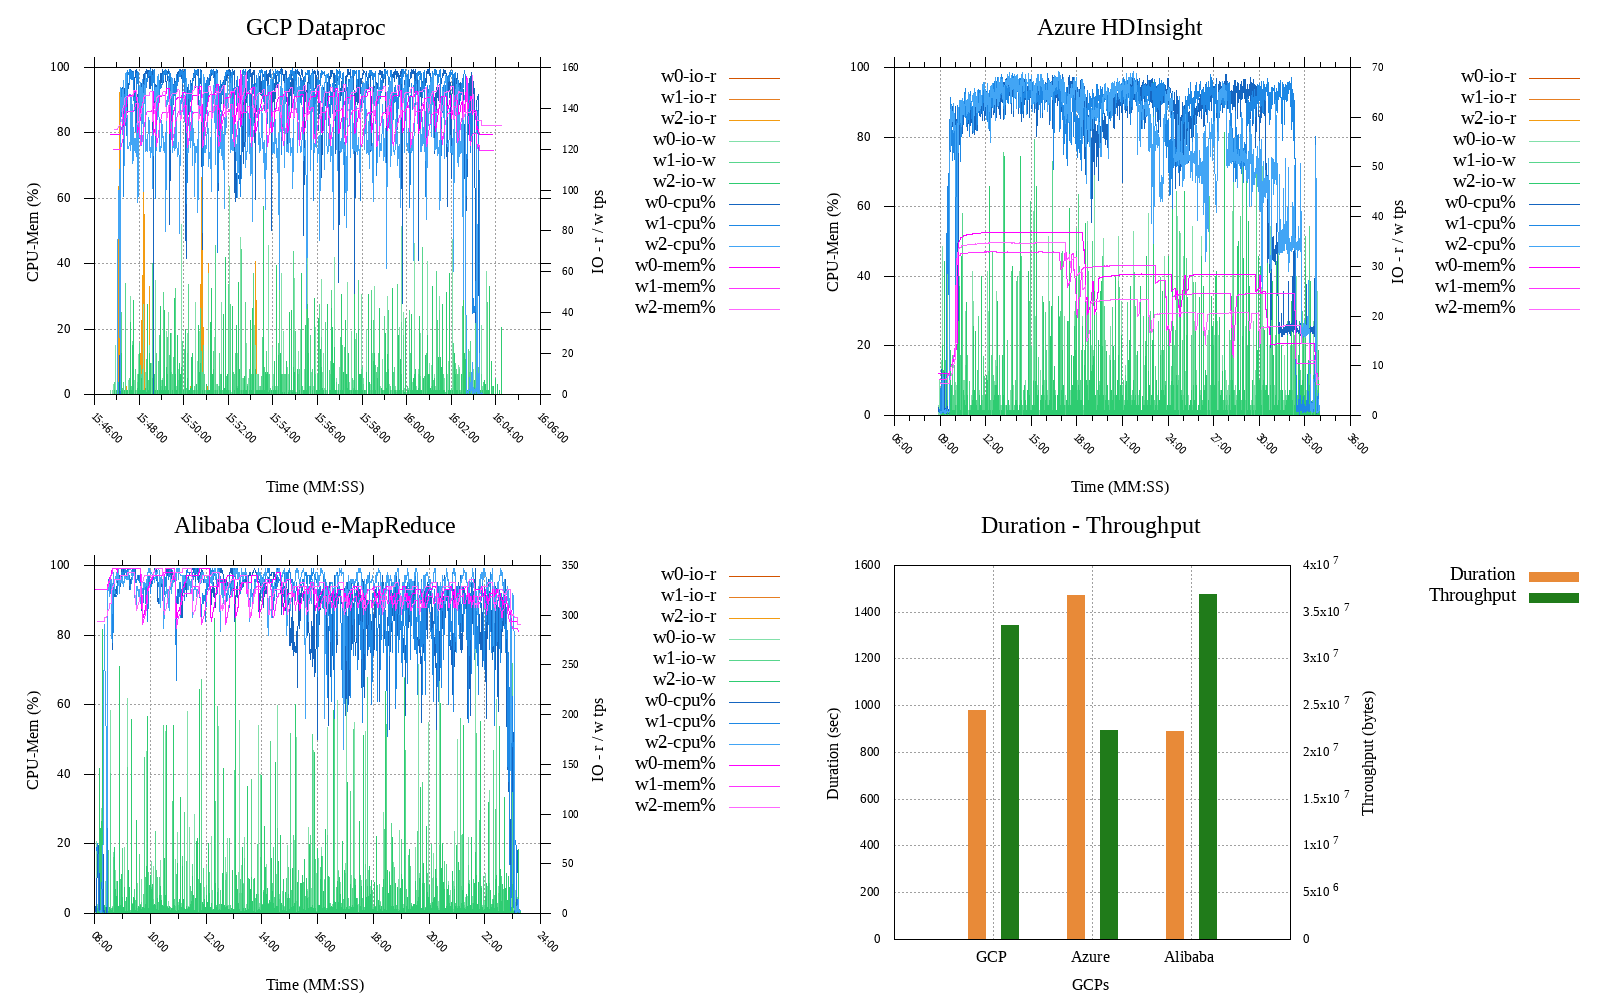
\includegraphics[width=\textwidth]{uc1-wrdcnt-h-cmidt}
	\caption{UC1 - Wordcount (Huge; 32 GB)}
	\label{fig:uc1-wrdcnt-h-cmidt}
	\centering
\end{figure}

\begin{figure}[b]
	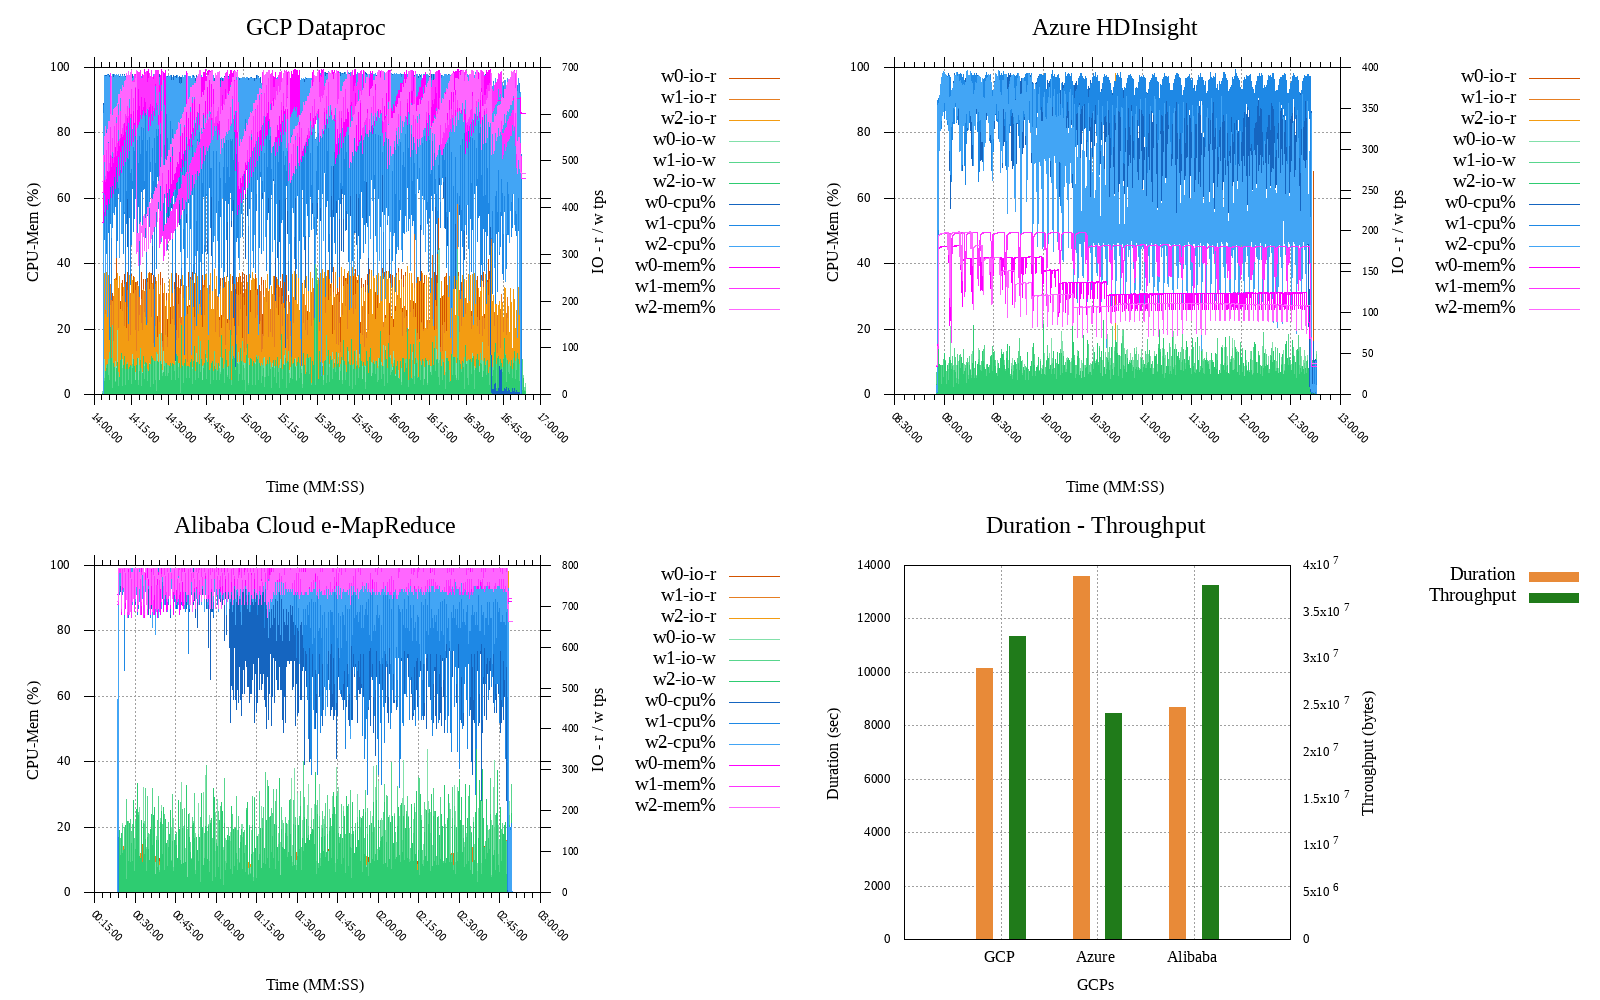
\includegraphics[width=\textwidth]{uc1-wrdcnt-g-cmidt}
	\caption{UC1 - Wordcount (Gigantic; 320 GB)}
	\label{fig:uc1-wrdcnt-g-cmidt}
	\centering
\end{figure}

\begin{figure}[b]
	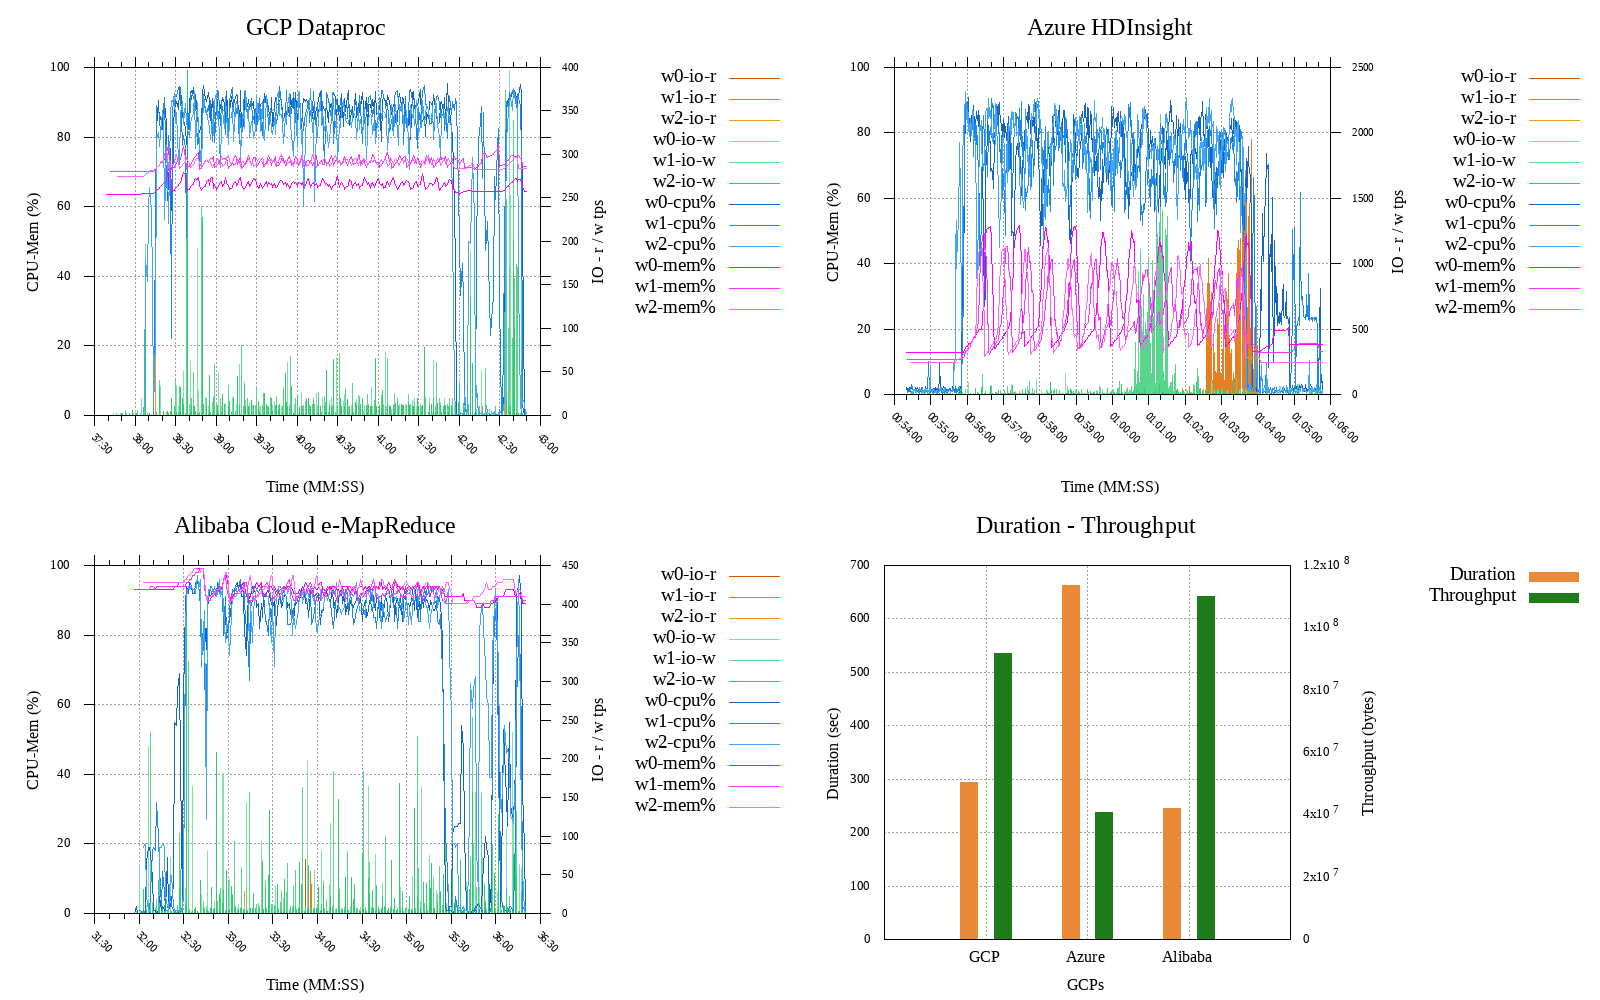
\includegraphics[width=\textwidth]{uc1-dfsioer-h-cmidt}
	\caption{UC1 - Dfsioe-read (Huge; No of Files: 256, File size: 100 MB)}
	\label{fig:uc1-dfsioer-h-cmidt}
	\centering
\end{figure}

\begin{figure}[b]
	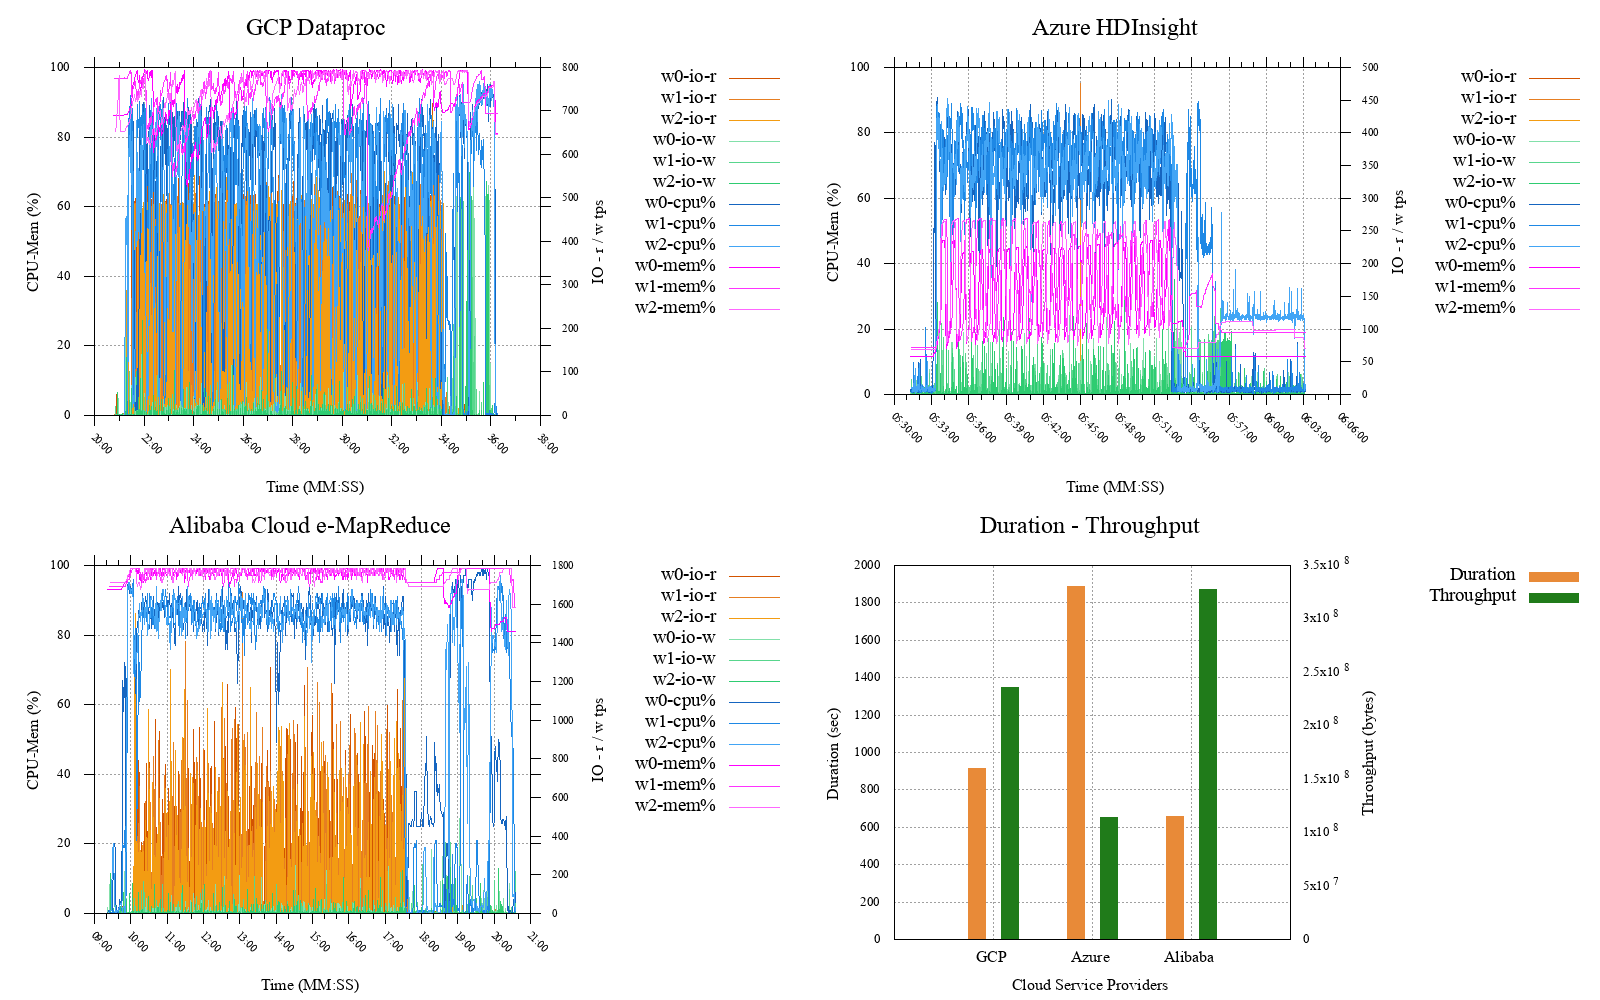
\includegraphics[width=\textwidth]{uc1-dfsioer-g-cmidt}
	\caption{UC1 - Dfsioe-read (Gigantic; No of Files: 512, File size: 400 MB)}
	\label{fig:uc1-dfsioer-g-cmidt}
	\centering
\end{figure}

\begin{figure}[b]
	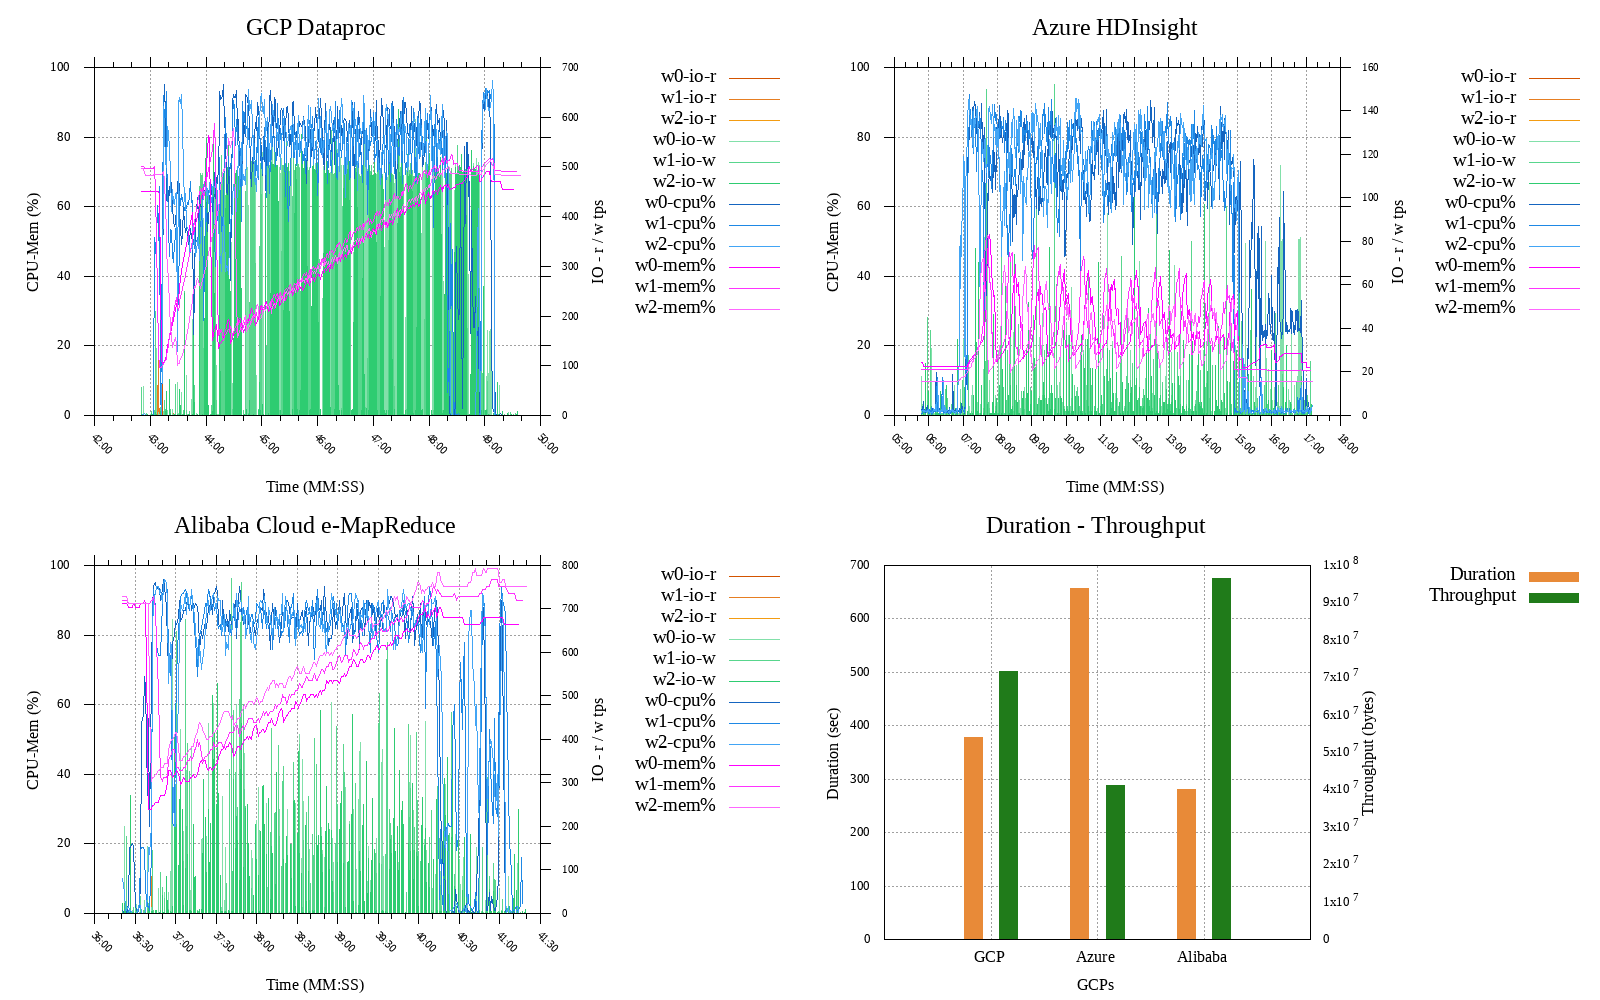
\includegraphics[width=\textwidth]{uc1-dfsioew-h-cmidt}
	\caption{UC1 - Dfsioe-write (Huge; No of Files: 256, File size: 100 MB)}
	\label{fig:uc1-dfsioew-h-cmidt}
	\centering
\end{figure}

\begin{figure}[b]
	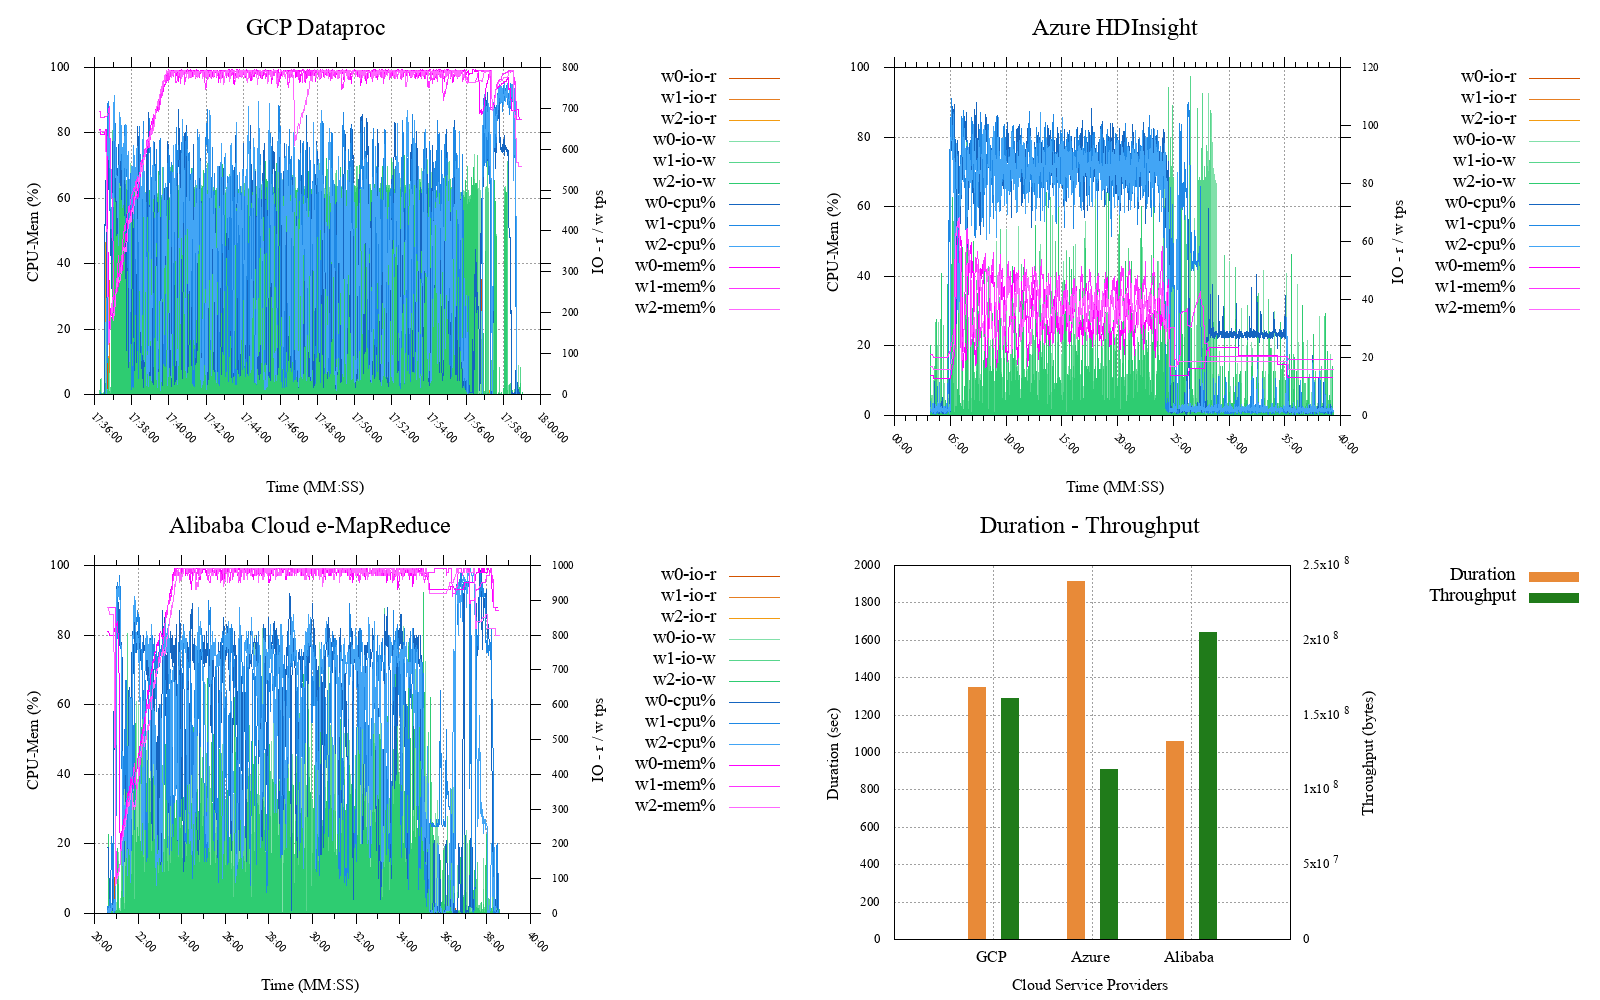
\includegraphics[width=\textwidth]{uc1-dfsioew-g-cmidt}
	\caption{UC1 - Dfsioe-write (Gigantic; No of Files: 512, File size: 400 MB)}
	\label{fig:uc1-dfsioew-g-cmidt}
	\centering
\end{figure}

\begin{figure}[b]
	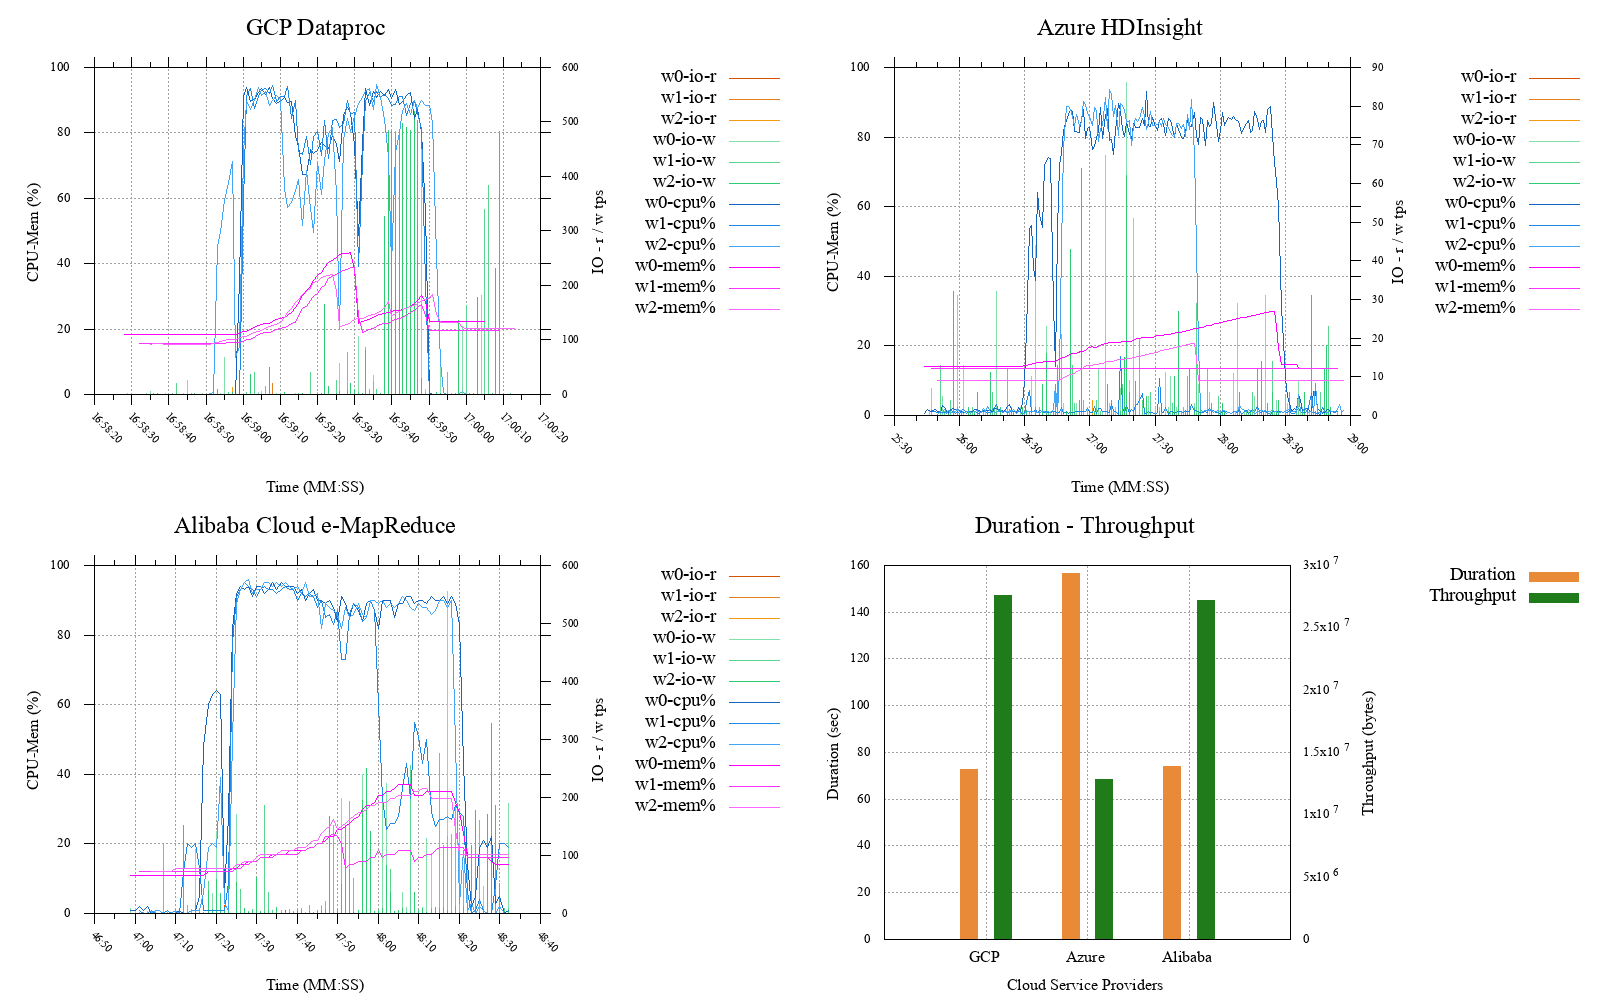
\includegraphics[width=\textwidth]{uc1-scan-h-cmidt}
	\caption{UC1 - Scan (Huge; USERVISITS: 10,000,000 PAGES: 1,200,000)}
	\label{fig:uc1-scan-h-cmidt}
	\centering
\end{figure}

\begin{figure}[b]
	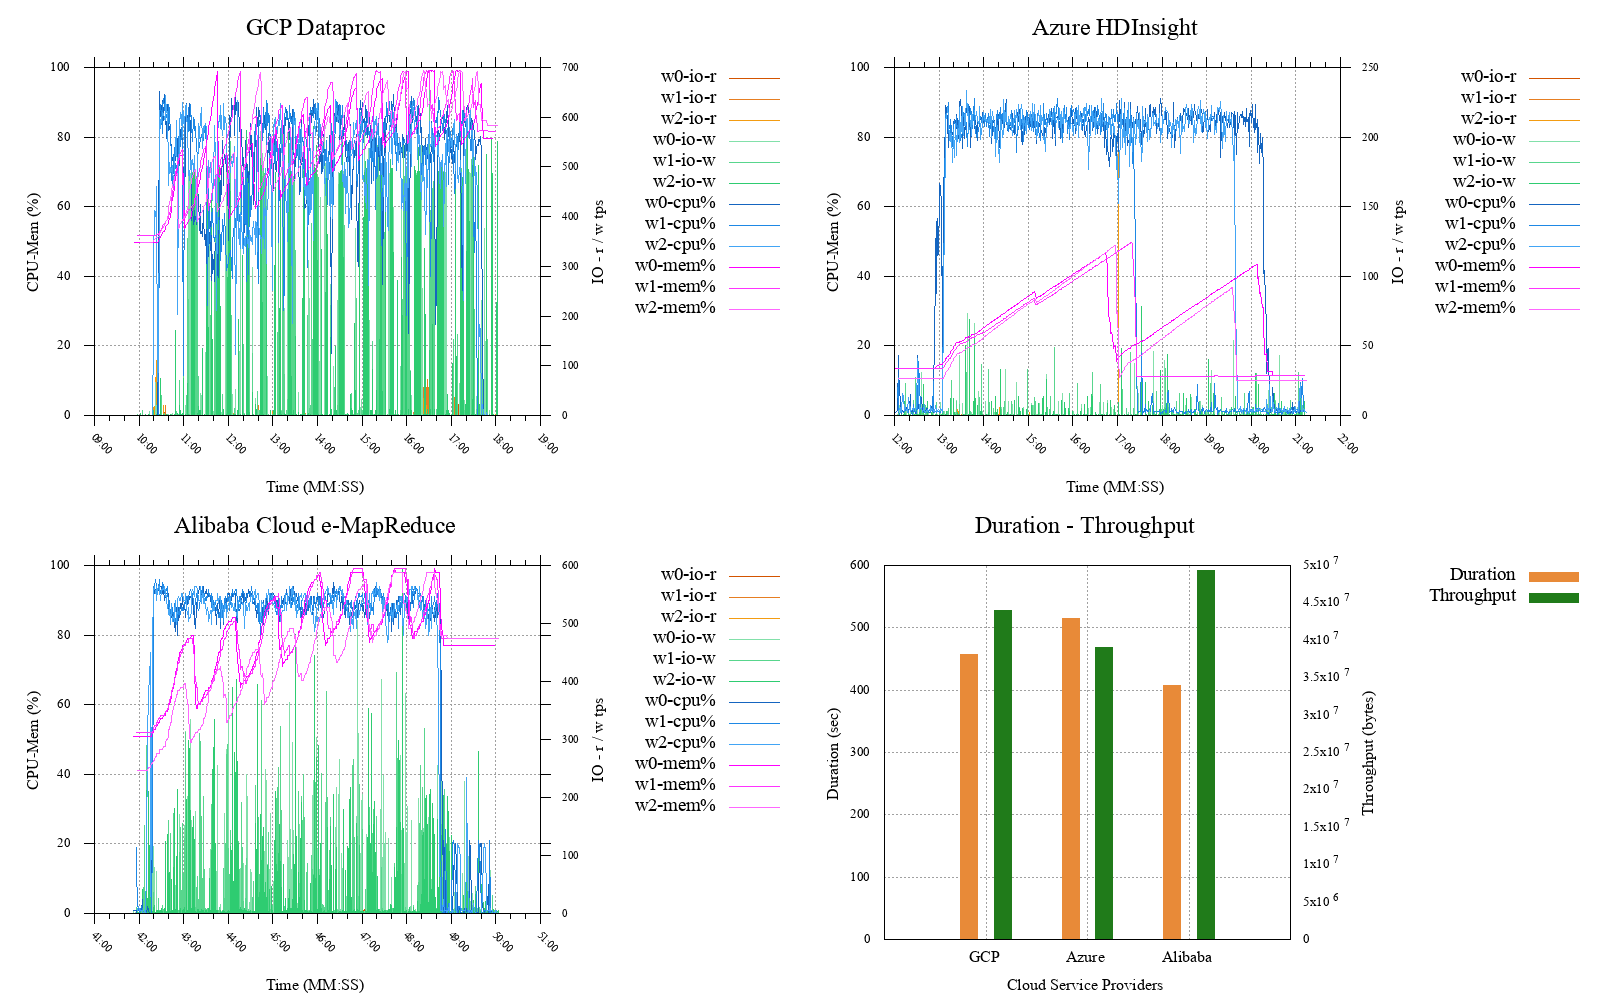
\includegraphics[width=\textwidth]{uc1-scan-g-cmidt}
	\caption{UC1 - Scan (Gigantic; USERVISITS: 100,000,000 PAGES: 12,000,000)}
	\label{fig:uc1-scan-g-cmidt}
	\centering
\end{figure}

\begin{figure}[b]
	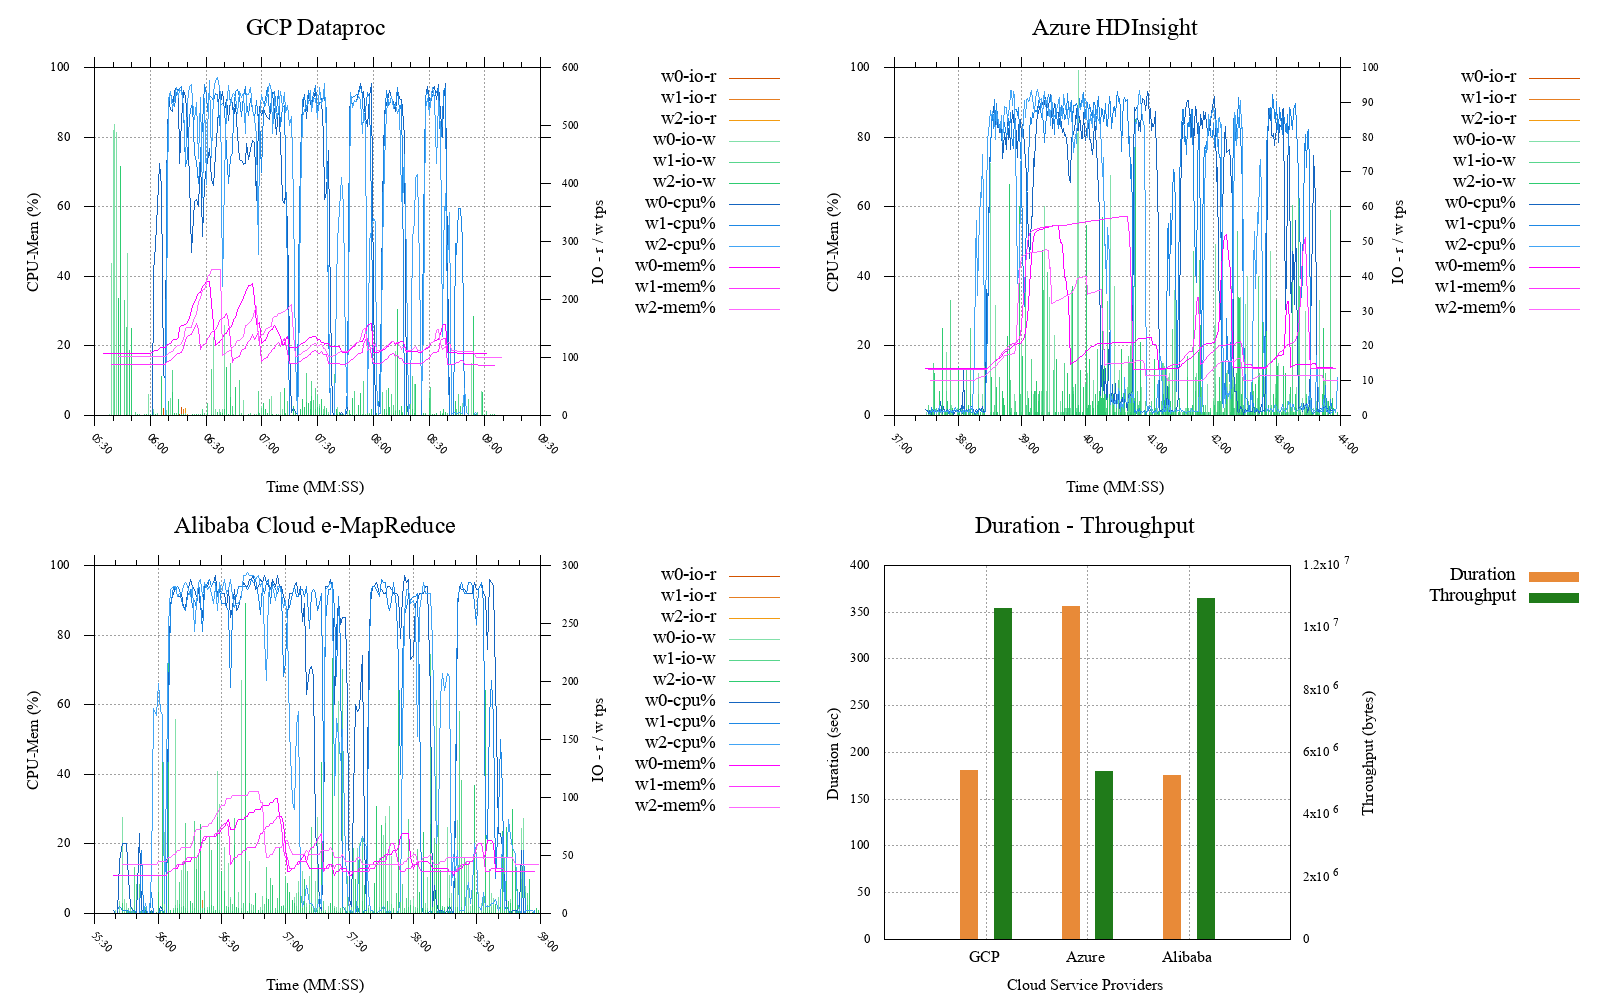
\includegraphics[width=\textwidth]{uc1-join-h-cmidt}
	\caption{UC1 - Join (Huge; USERVISITS: 10,000,000 PAGES: 1,200,000)}
	\label{fig:uc1-join-h-cmidt}
	\centering
\end{figure}

\begin{figure}[b]
	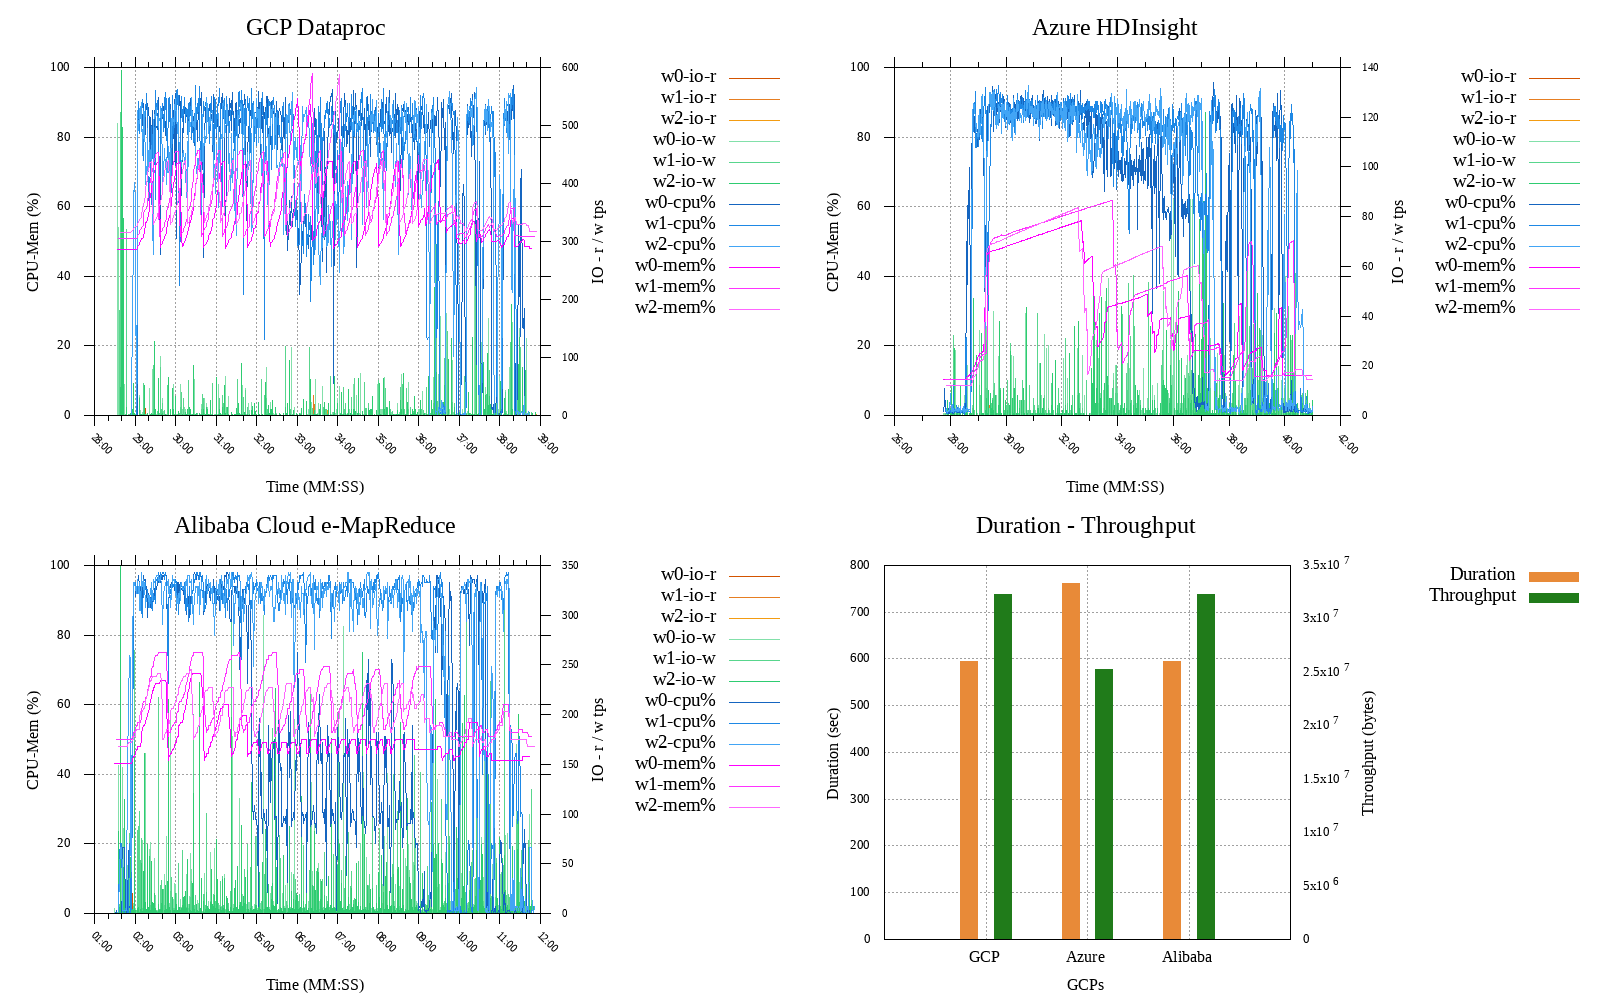
\includegraphics[width=\textwidth]{uc1-join-g-cmidt}
	\caption{UC1 - Join (Gigantic; USERVISITS: 100,000,000 PAGES: 12,000,000)}
	\label{fig:uc1-join-g-cmidt}
	\centering
\end{figure}

\begin{figure}[b]
	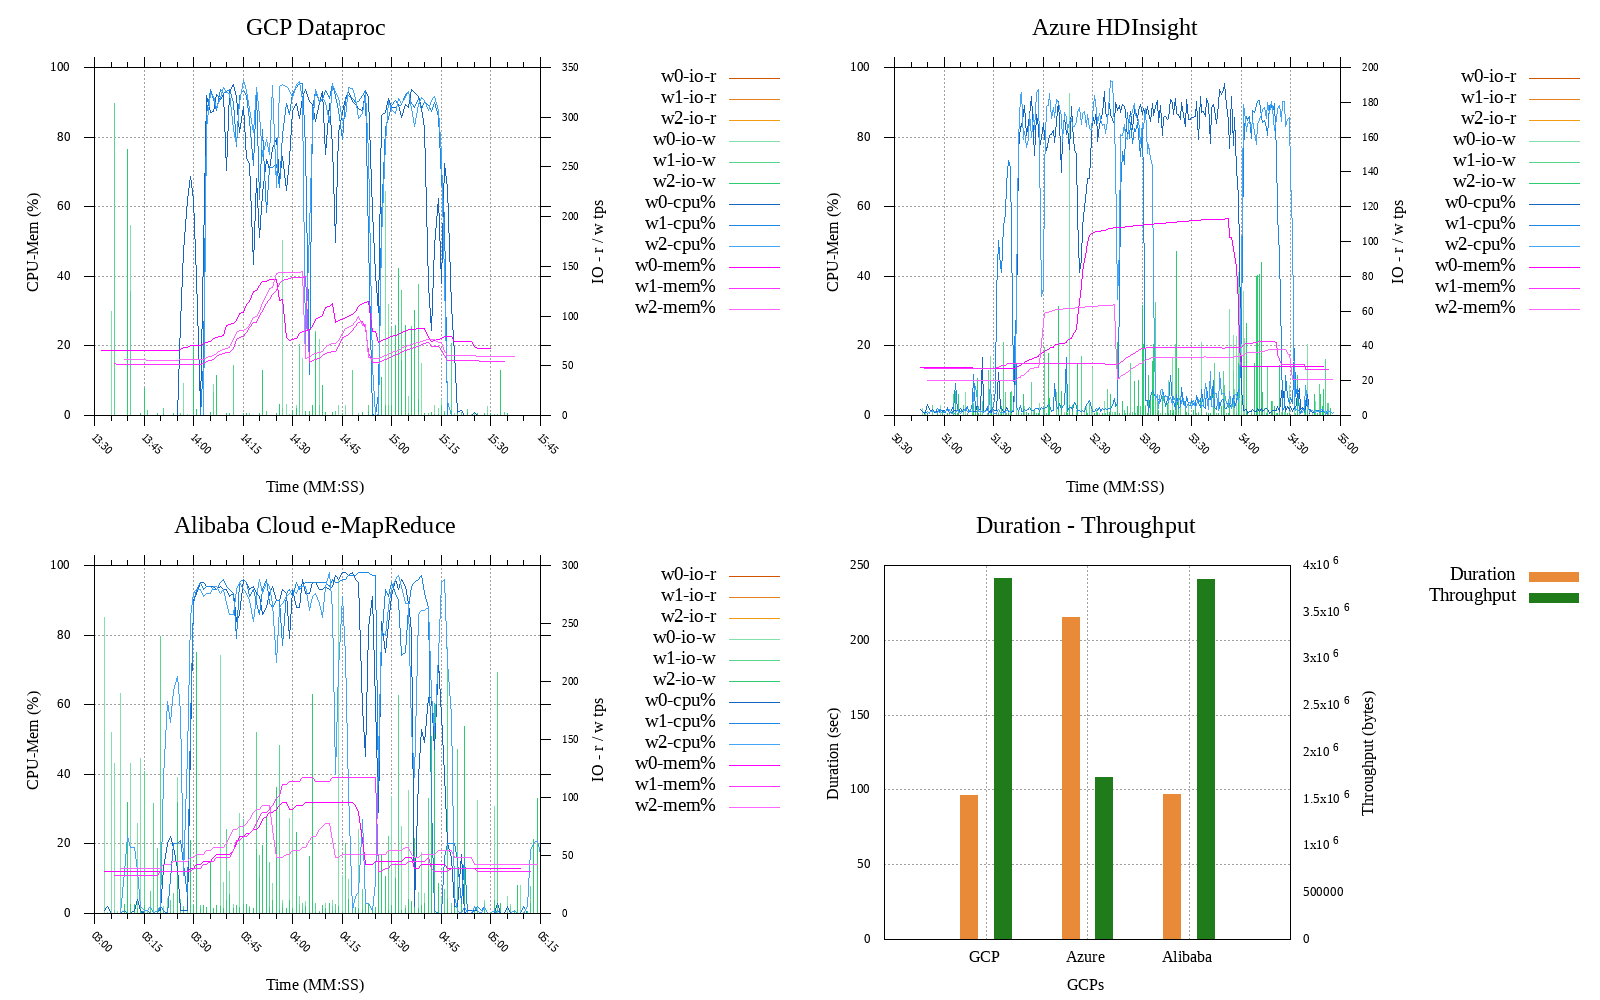
\includegraphics[width=\textwidth]{uc1-aggreg-h-cmidt}
	\caption{UC1 - Aggregation (Huge; USERVISITS: 10,000,000 PAGES: 1,200,000)}
	\label{fig:uc1-aggreg-h-cmidt}
	\centering
\end{figure}

\begin{figure}[b]
	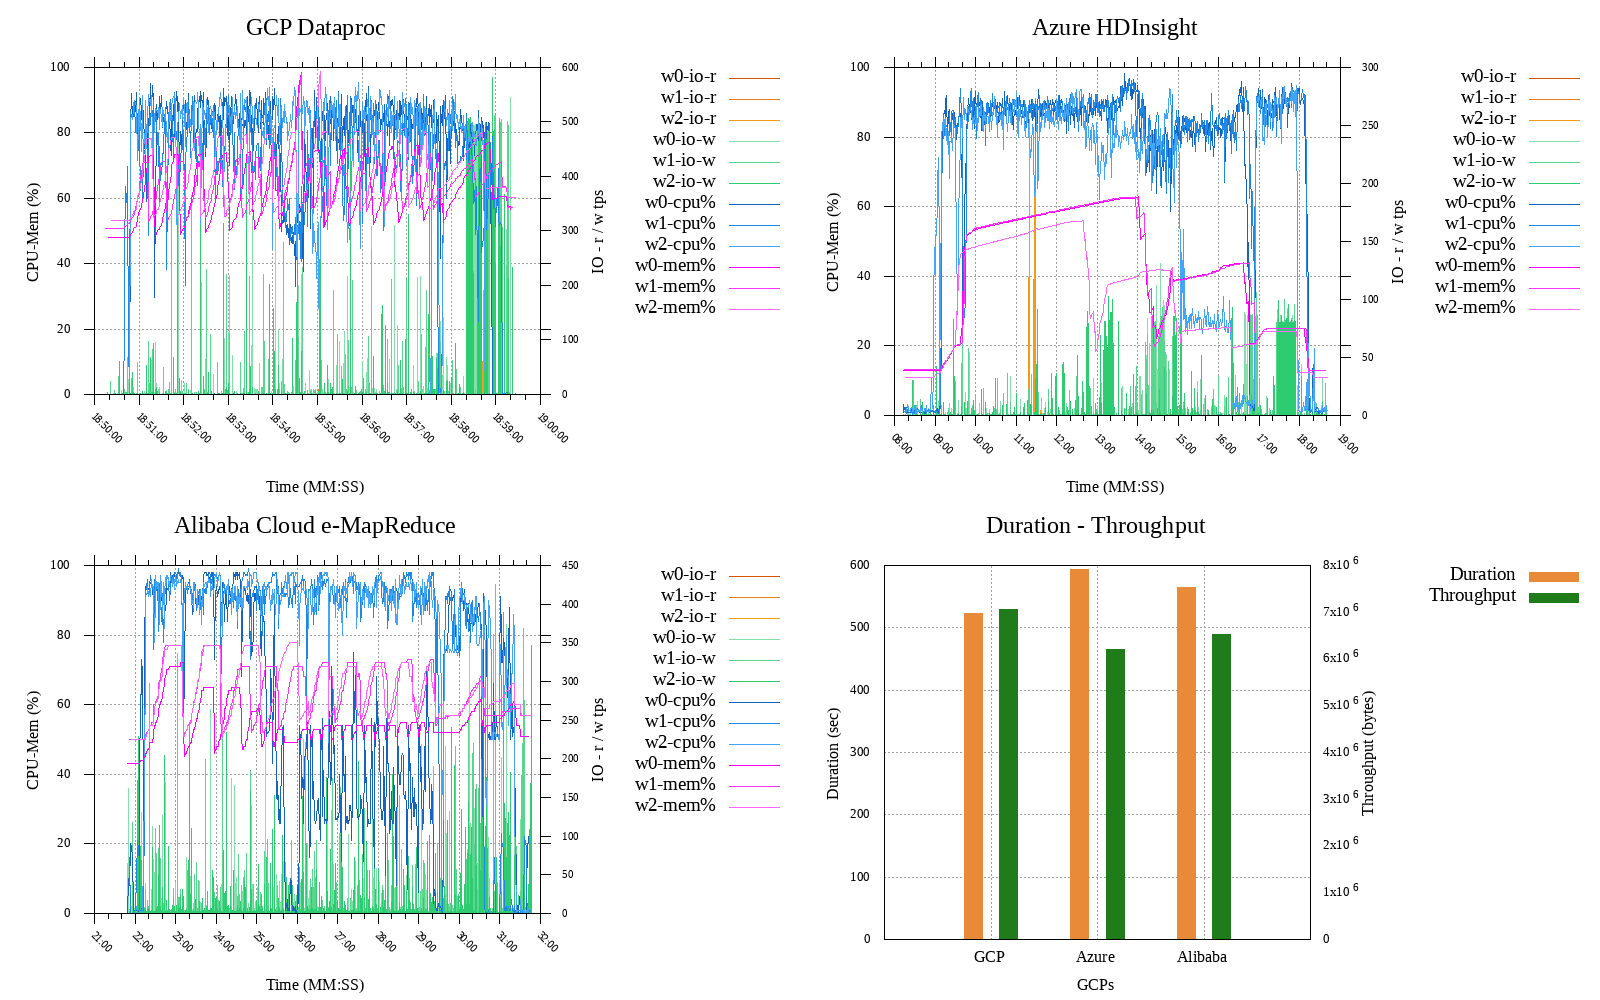
\includegraphics[width=\textwidth]{uc1-aggreg-g-cmidt}
	\caption{UC1 - Aggregation (Gigantic; USERVISITS: 100,000,000 PAGES: 12,000,000)}
	\label{fig:uc1-aggreg-g-cmidt}
	\centering
\end{figure}

\begin{figure}b]
	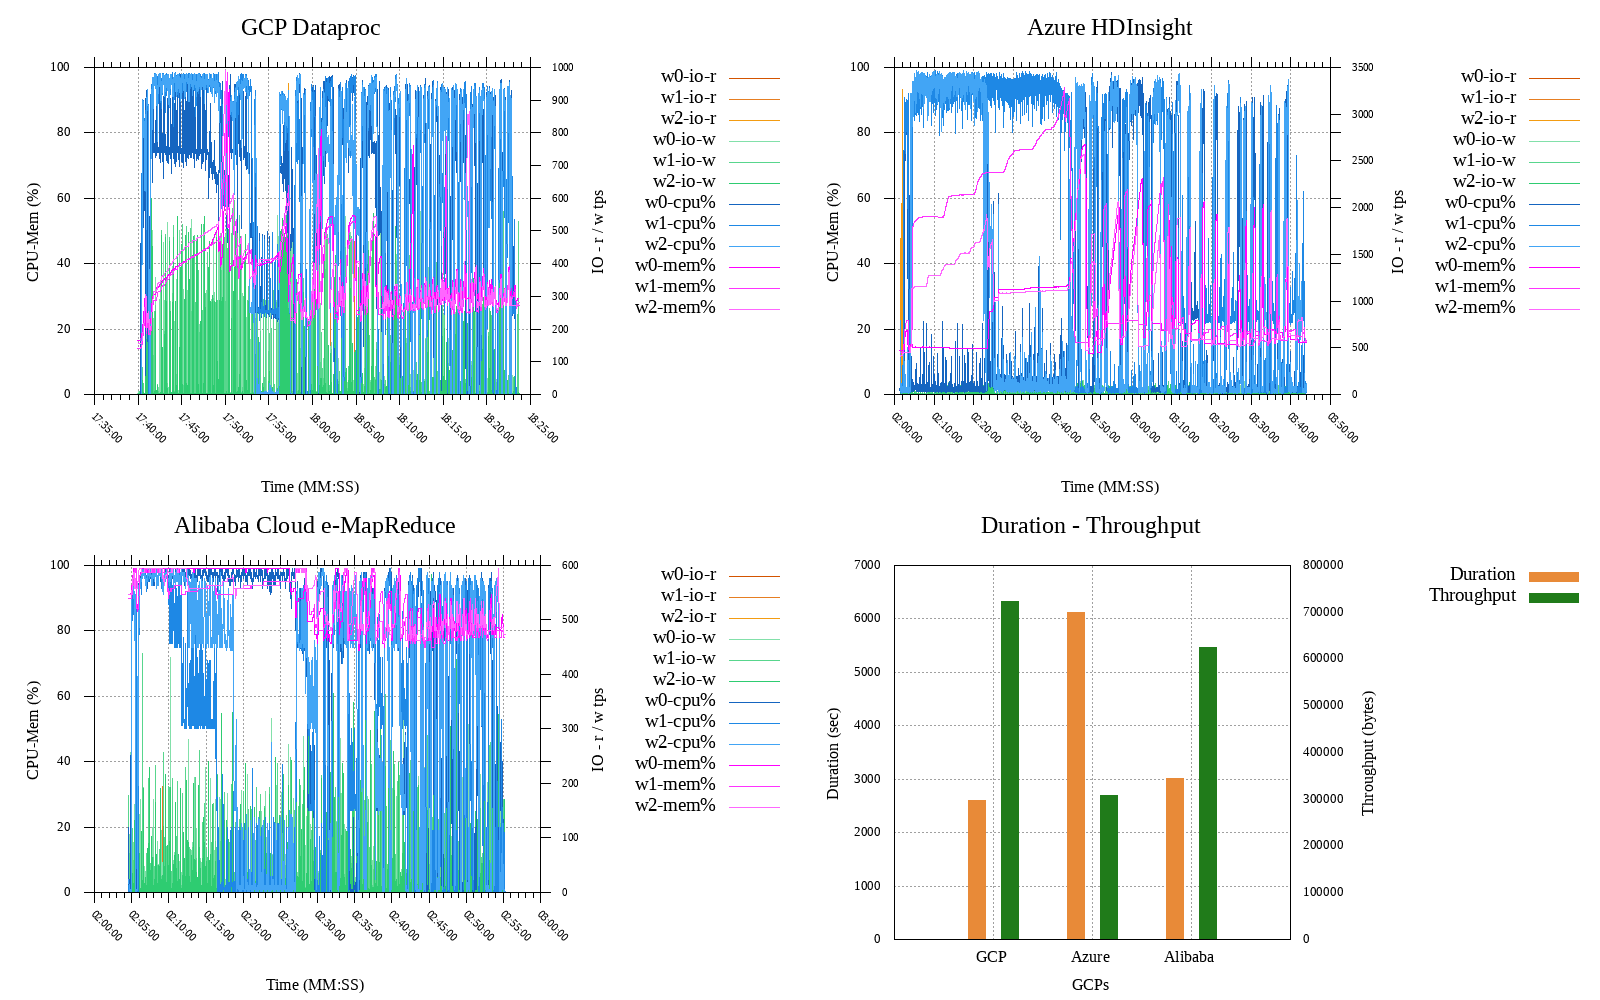
\includegraphics[width=\textwidth]{uc1-bayes-h-cmidt}
	\caption{UC1 - Bayes (Huge; PAGES: 500,000 CLASSES: 100 NGRAMS: 2)}
	\label{fig:uc1-bayes-h-cmidt}
	\centering
\end{figure}

\begin{figure}[b]
	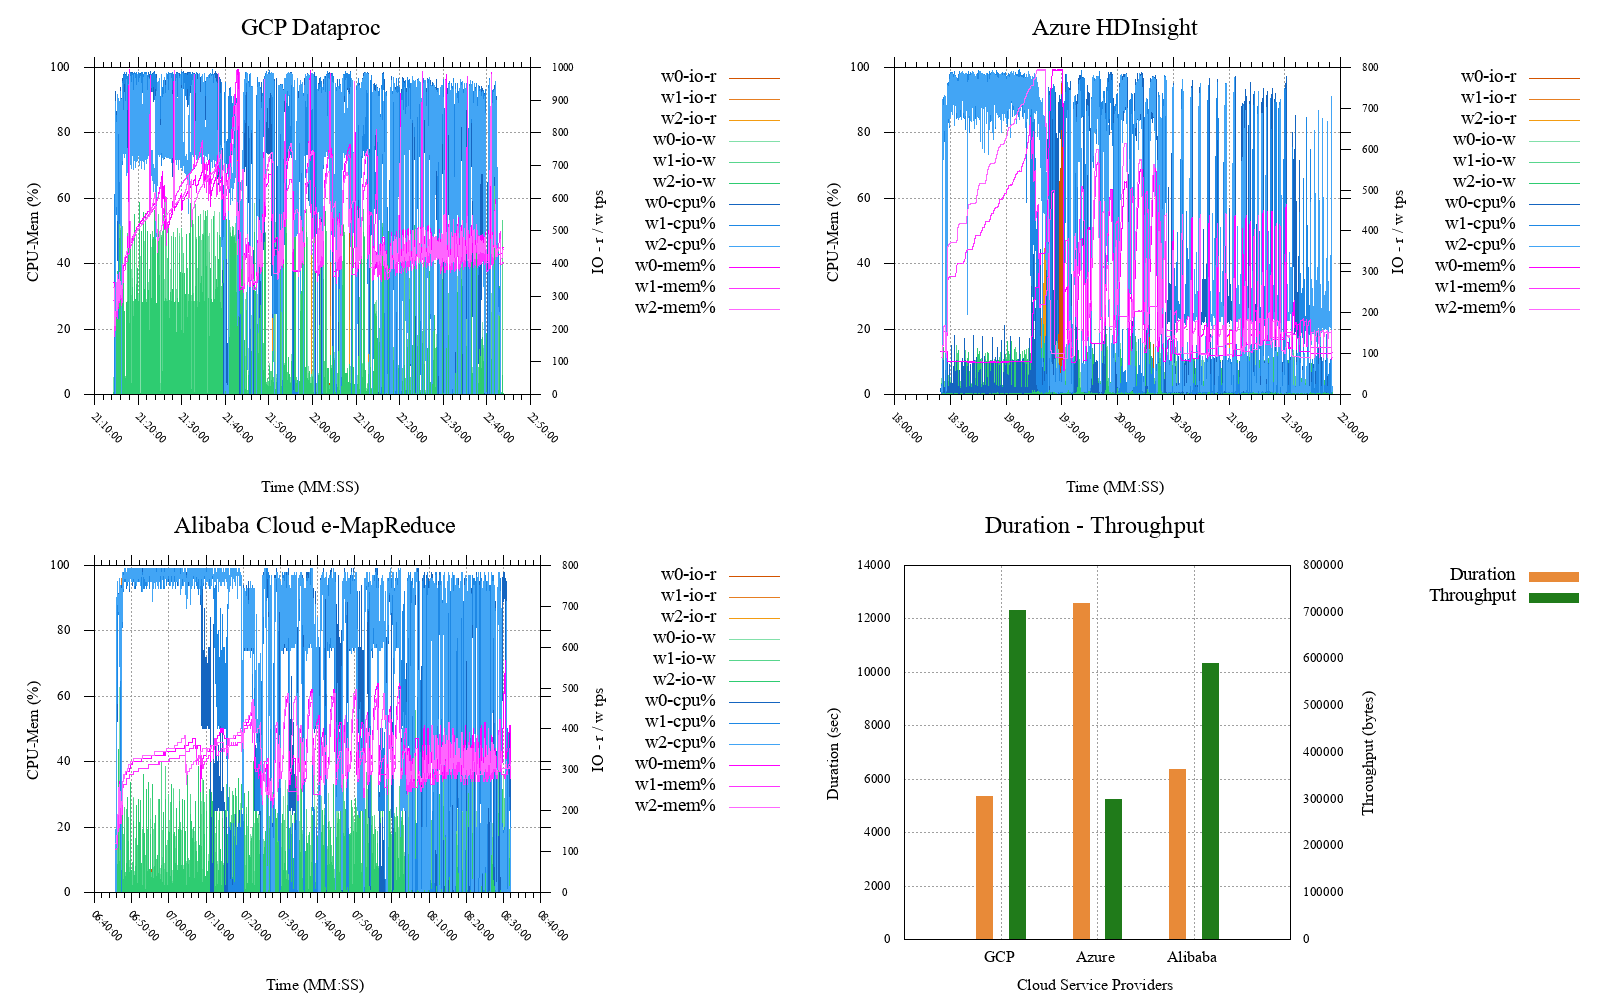
\includegraphics[width=\textwidth]{uc1-bayes-g-cmidt}
	\caption{UC1 - Bayes (Gigantic; PAGES: 1,000,000 CLASSES: 100 NGRAMS: 2)}
	\label{fig:uc1-bayes-g-cmidt}
	\centering
\end{figure}

\begin{figure}[b]
	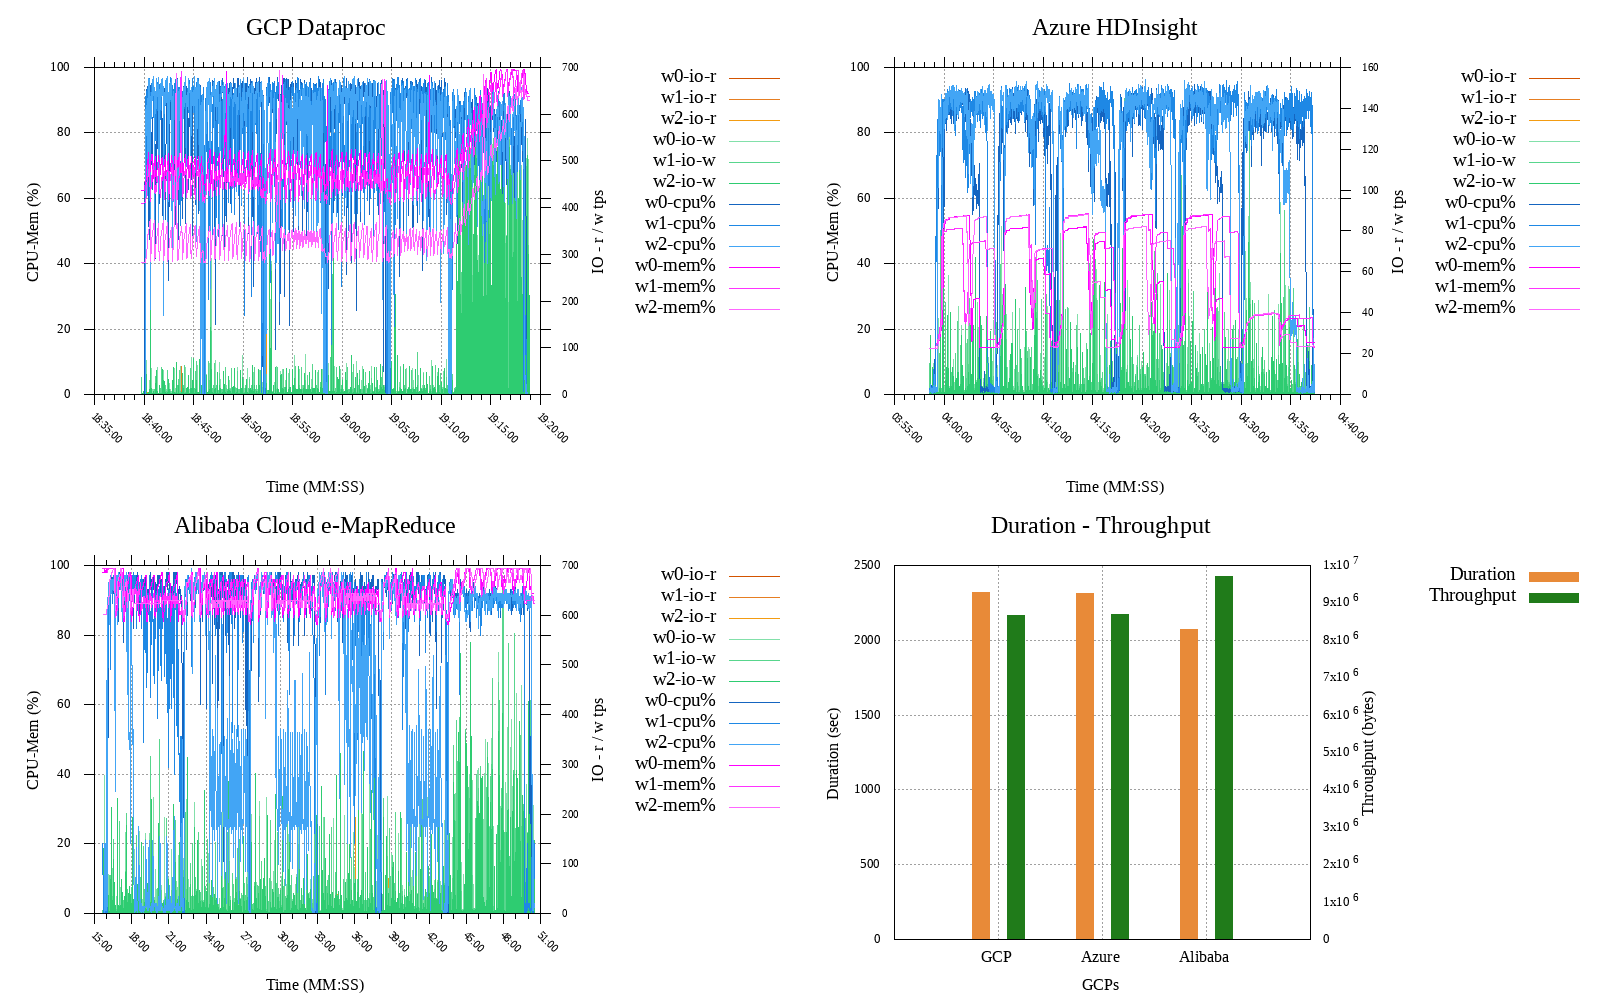
\includegraphics[width=\textwidth]{uc1-kmeans-h-cmidt}
	\caption{UC1 - Kmeans (Huge; CLUSTERS: 5 DIMENSIONS: 20 SAMPLES: 100,000,000 SAMP PER INPUT: 20,000,000 MAX IT: 5 K: 10 CONVERGEDIST: 0.5)}
	\label{fig:uc1-kmeans-h-cmidt}
	\centering
\end{figure}

\begin{figure}[b]
	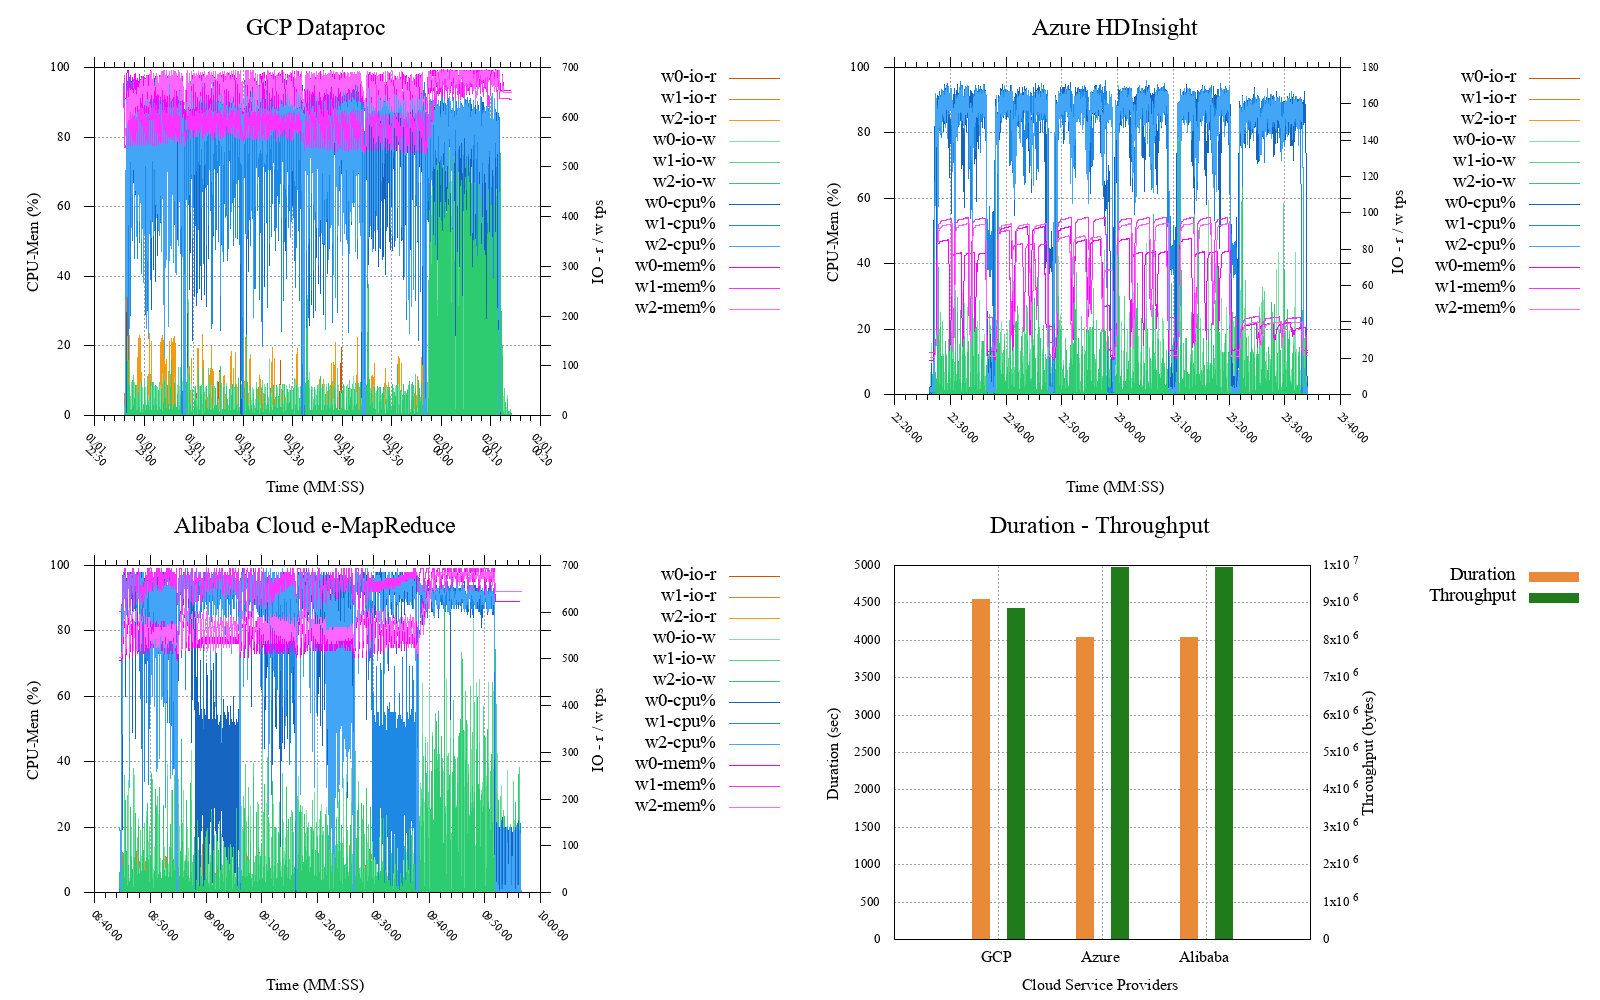
\includegraphics[width=\textwidth]{uc1-kmeans-g-cmidt}
	\caption{UC1 - Kmeans (Gigantic; CLUSTERS: 5 DIMENSIONS: 20 SAMPLES: 200,000,000 SAMP PER INPUT: 40,000,000 MAX IT: 5 K: 10 CONVERGEDIST: 0.5)}
	\label{fig:uc1-kmeans-g-cmidt}
	\centering
\end{figure}

\begin{figure}[b]
	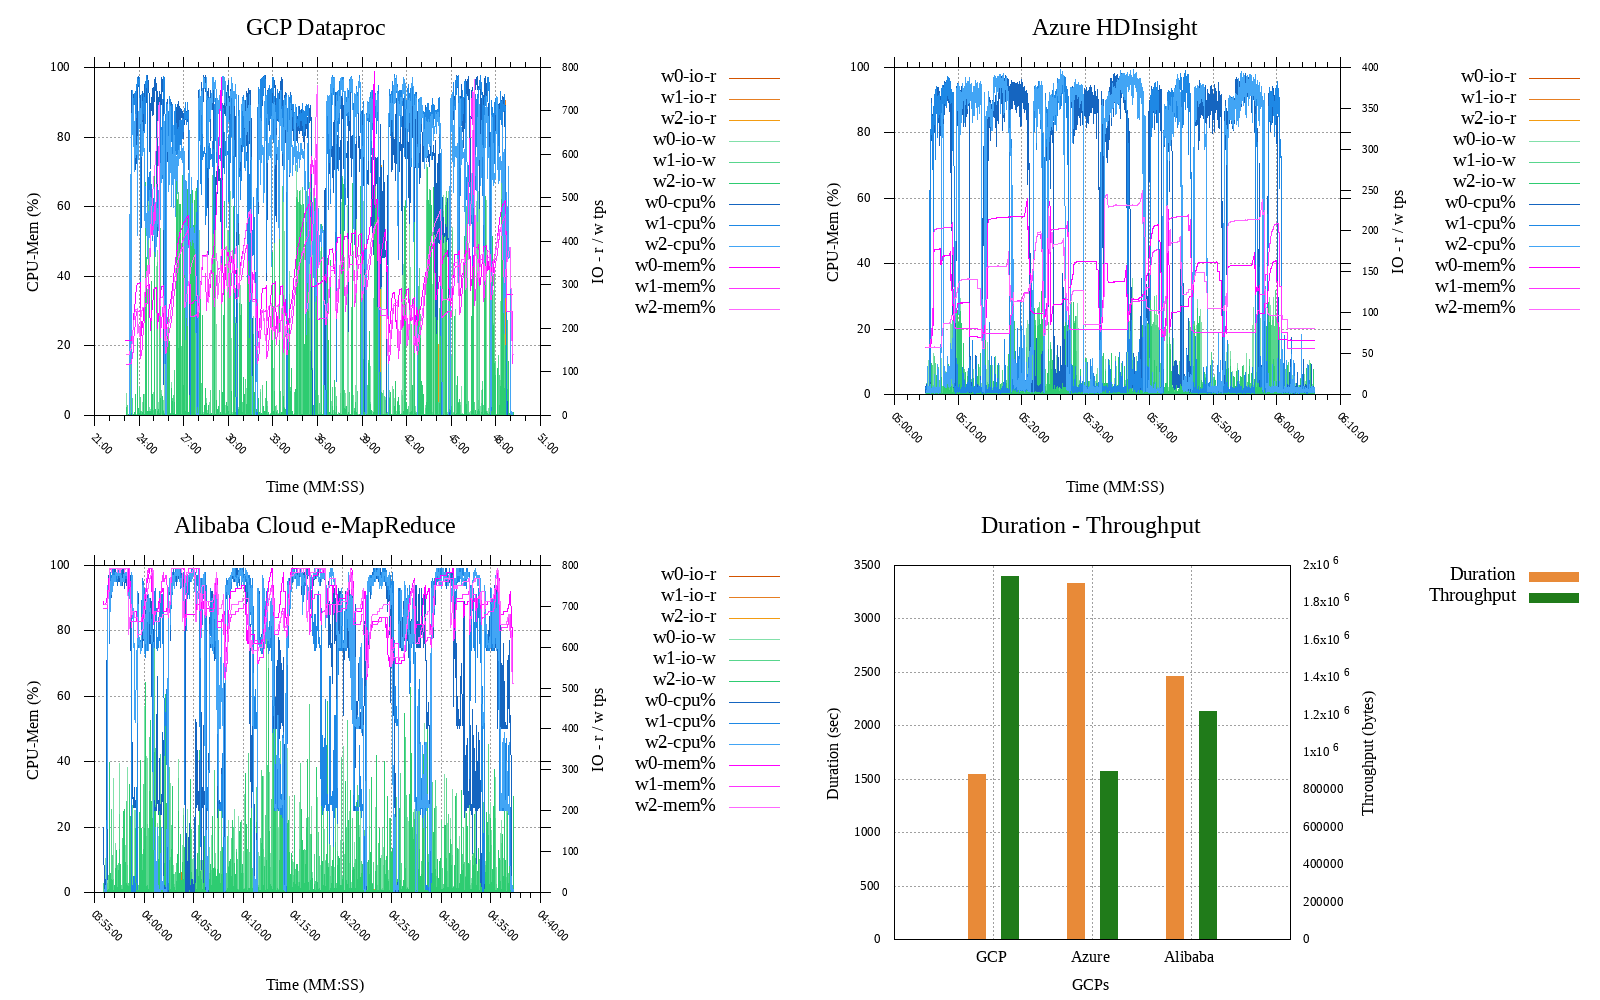
\includegraphics[width=\textwidth]{uc1-page-h-cmidt}
	\caption{UC1 - Pagerank (Huge; PAGES: 5,000,000 NUM ITERATIONS: 3 BLOCK: 0 BLOCK WIDTH: 16)}
	\label{fig:uc1-page-h-cmidt}
	\centering
\end{figure}

\begin{figure}[b]
	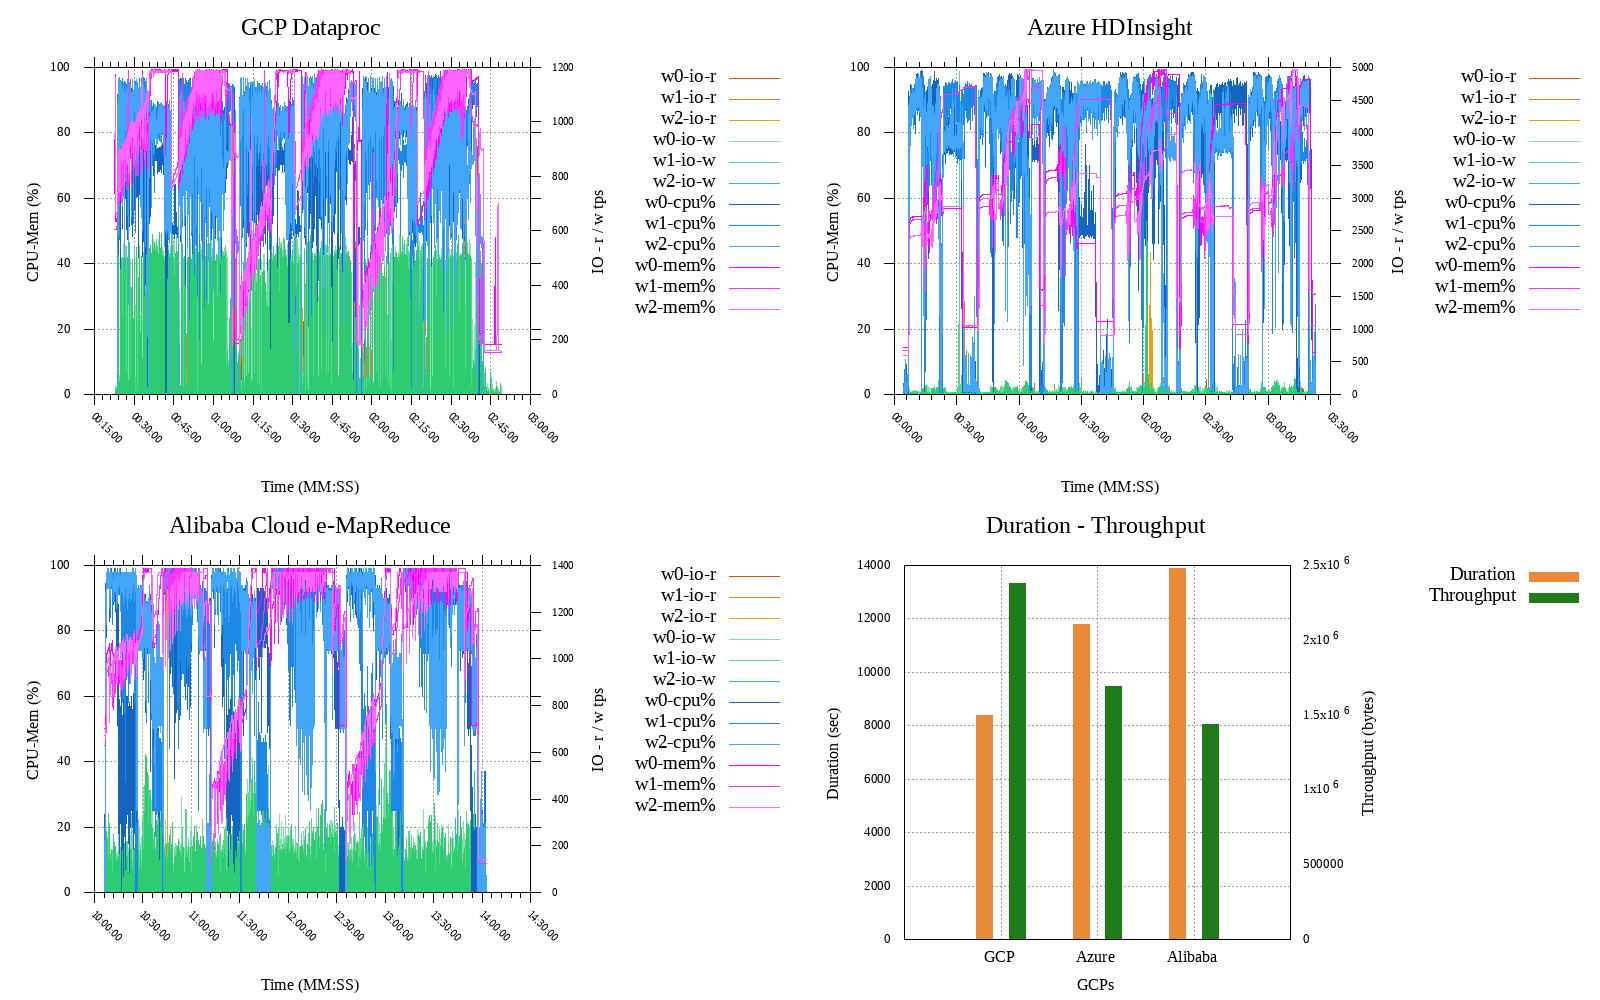
\includegraphics[width=\textwidth]{uc1-page-g-cmidt}
	\caption{UC1 - Pagerank (Gigantic; PAGES: 30,000,000 NUM ITERATIONS: 3 BLOCK: 0 BLOCK WIDTH: 16)}
	\label{fig:uc1-page-g-cmidt}
	\centering
\end{figure}

A possible reason for Azure's downperformance in dfsioe over GCP and Alibaba





USE CASE 2: 

\paragraph{Sort} Figure \ref{fig:uc2-srt}; 
%\paragraph{Sort - Small} Figure \ref{fig:uc2-srt-s-cmidt}; 
%\paragraph{Sort - Large} Figure \ref{fig:uc2-srt-l-cmidt}; 
%\paragraph{Sort - Huge} Figure \ref{fig:uc2-srt-h-cmidt}; 
%\paragraph{Sort - Gigantic} Figure \ref{fig:uc2-srt-g-cmidt}; 



\paragraph{Wordcount} Figure \ref{fig:uc2-wrdcnt}; 
%\paragraph{Wordcount - Small} Figure \ref{fig:uc2-wrdcnt-s-cmidt}; 
%\paragraph{Wordcount - Large} Figure \ref{fig:uc2-wrdcnt-l-cmidt}; 
%\paragraph{Wordcount - Huge} Figure \ref{fig:uc2-wrdcnt-h-cmidt}; 
%\paragraph{Wordcount - Gigantic} Figure \ref{fig:uc2-wrdcnt-g-cmidt}; 


\begin{figure}[b]
	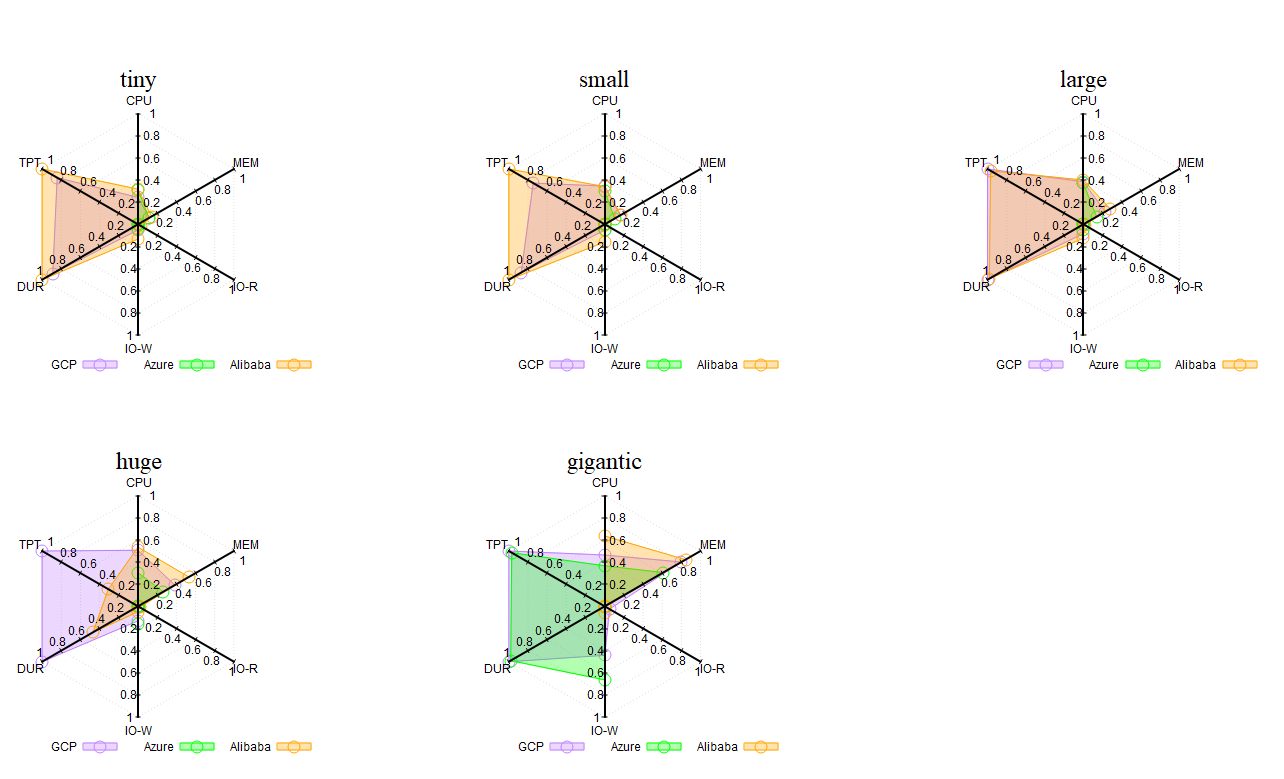
\includegraphics[width=\textwidth]{uc2-srt}
	\caption{Use Case 2 - Sort performances along data scales}
	\label{fig:uc2-srt}
	\centering
\end{figure}

\begin{figure}[b]
	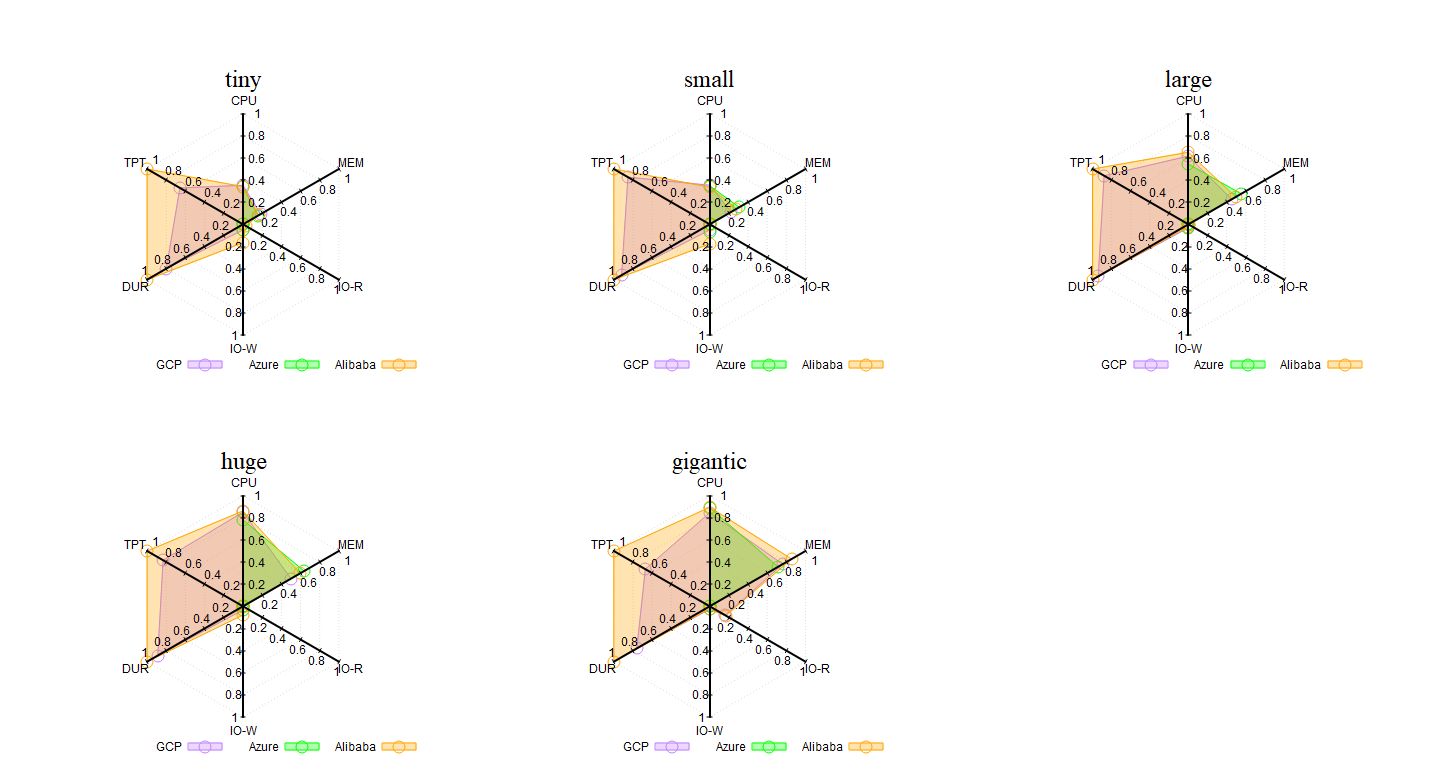
\includegraphics[width=\textwidth]{uc2-wrdcnt}
	\caption{Use Case 2 - Wordcount performances along data scales}
	\label{fig:uc2-wrdcnt}
	\centering
\end{figure}

%\begin{figure}[b]
%	\caption{UC2 - Sort (Tiny; 32 KB)}
%	\label{fig:uc2-srt-t-cmidt}
%	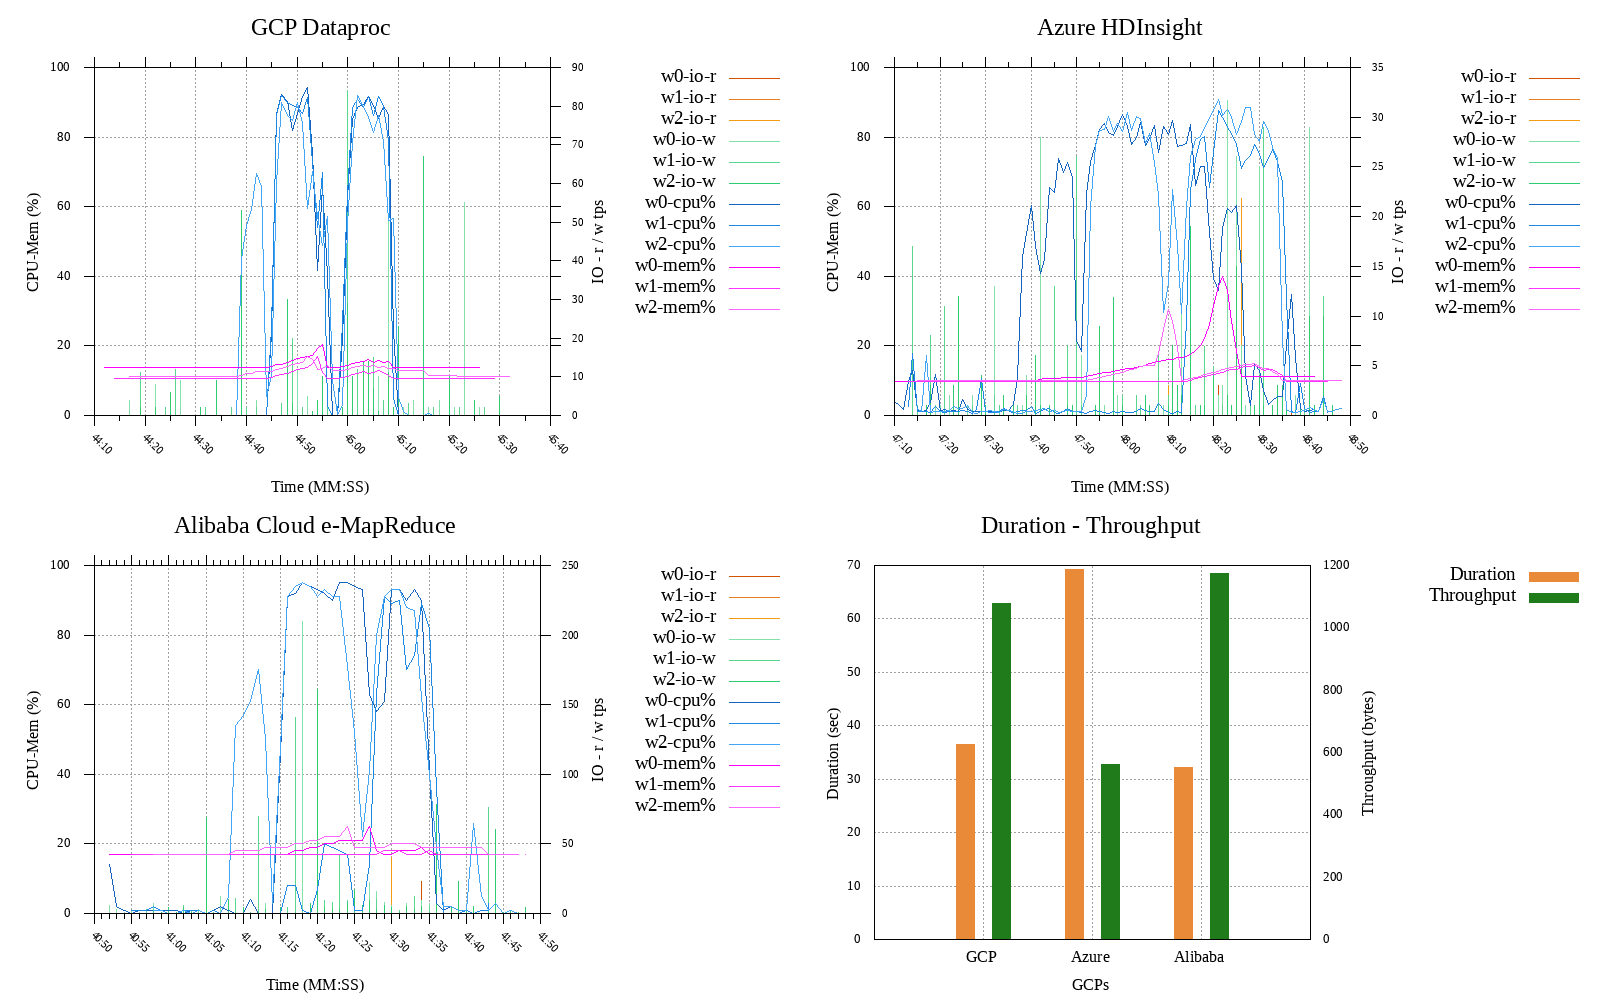
\includegraphics[width=\textwidth]{uc2-srt-t-cmidt}
%	\centering
%\end{figure}
%
%\begin{figure}[b]
%	\caption{UC2 - Sort (Small; 3.2 MB)}
%	\label{fig:uc2-srt-s-cmidt}
%	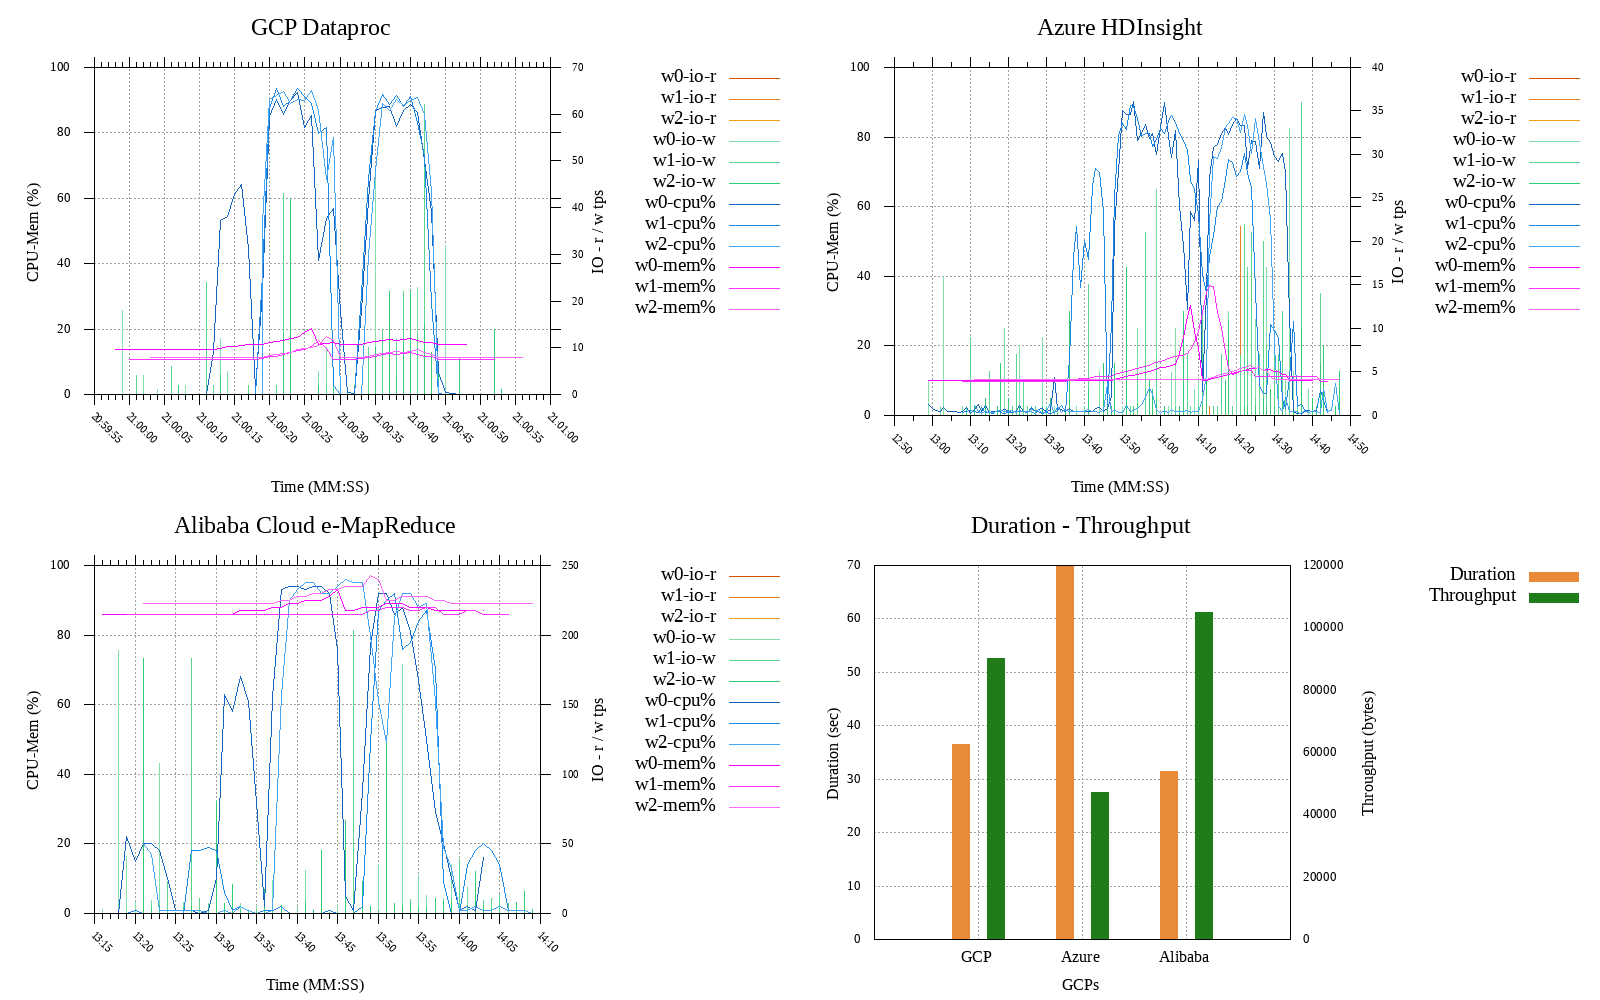
\includegraphics[width=\textwidth]{uc2-srt-s-cmidt}
%	\centering
%\end{figure}
%
%\begin{figure}[b]
%	\caption{UC2 - Sort (Large; 320 MB)}
%	\label{fig:uc2-srt-l-cmidt}
%	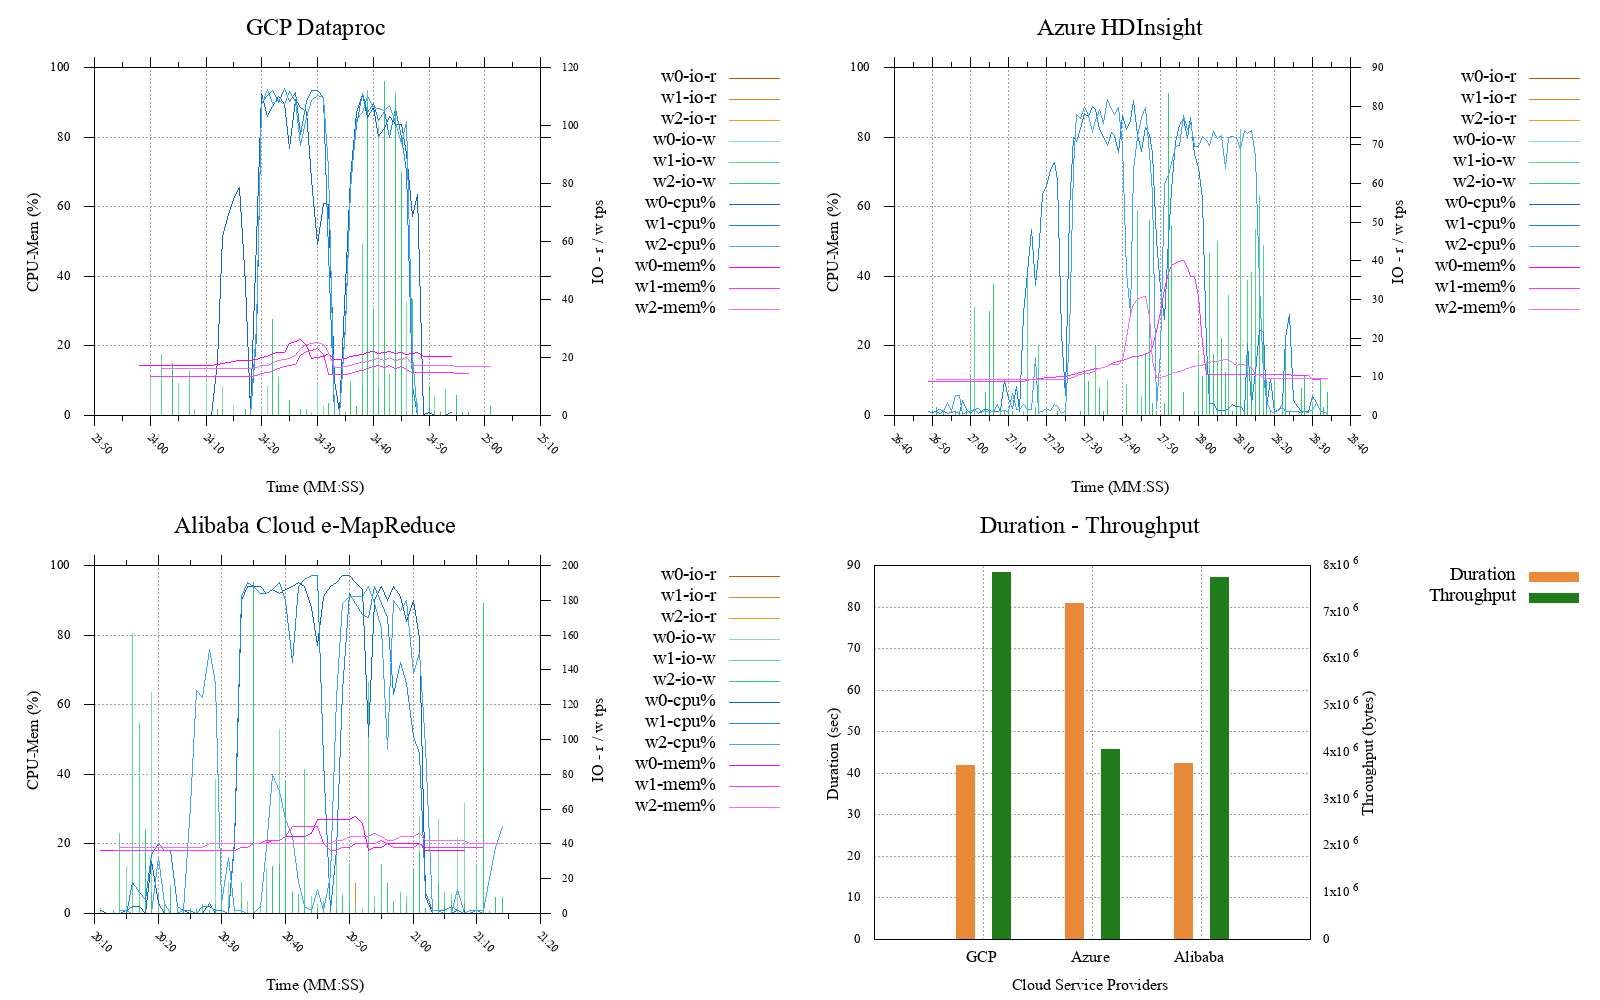
\includegraphics[width=\textwidth]{uc2-srt-l-cmidt}
%	\centering
%\end{figure}
%
%\begin{figure}[b]
%	\caption{UC2 - Sort (Huge; 3.2 GB)}
%	\label{fig:uc2-srt-h-cmidt}
%	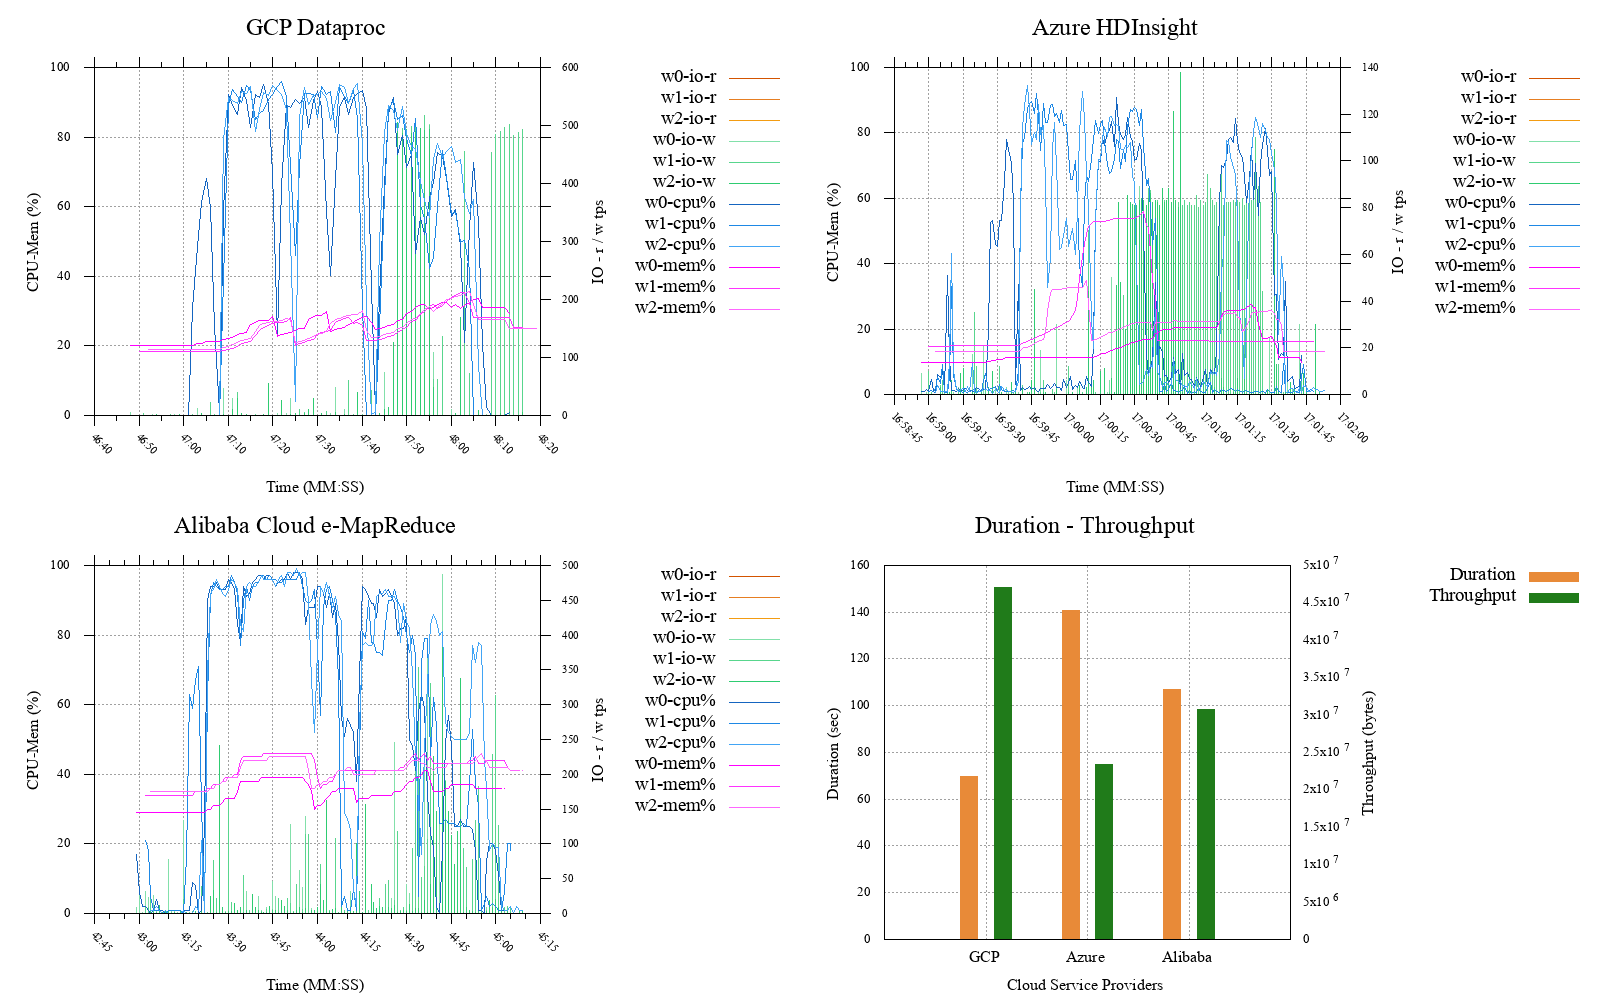
\includegraphics[width=\textwidth]{uc2-srt-h-cmidt}
%	\centering
%\end{figure}
%
%\begin{figure}[b]
%	\caption{UC2 - Sort (Gigantic; 32 GB)}
%	\label{fig:uc2-srt-g-cmidt}
%	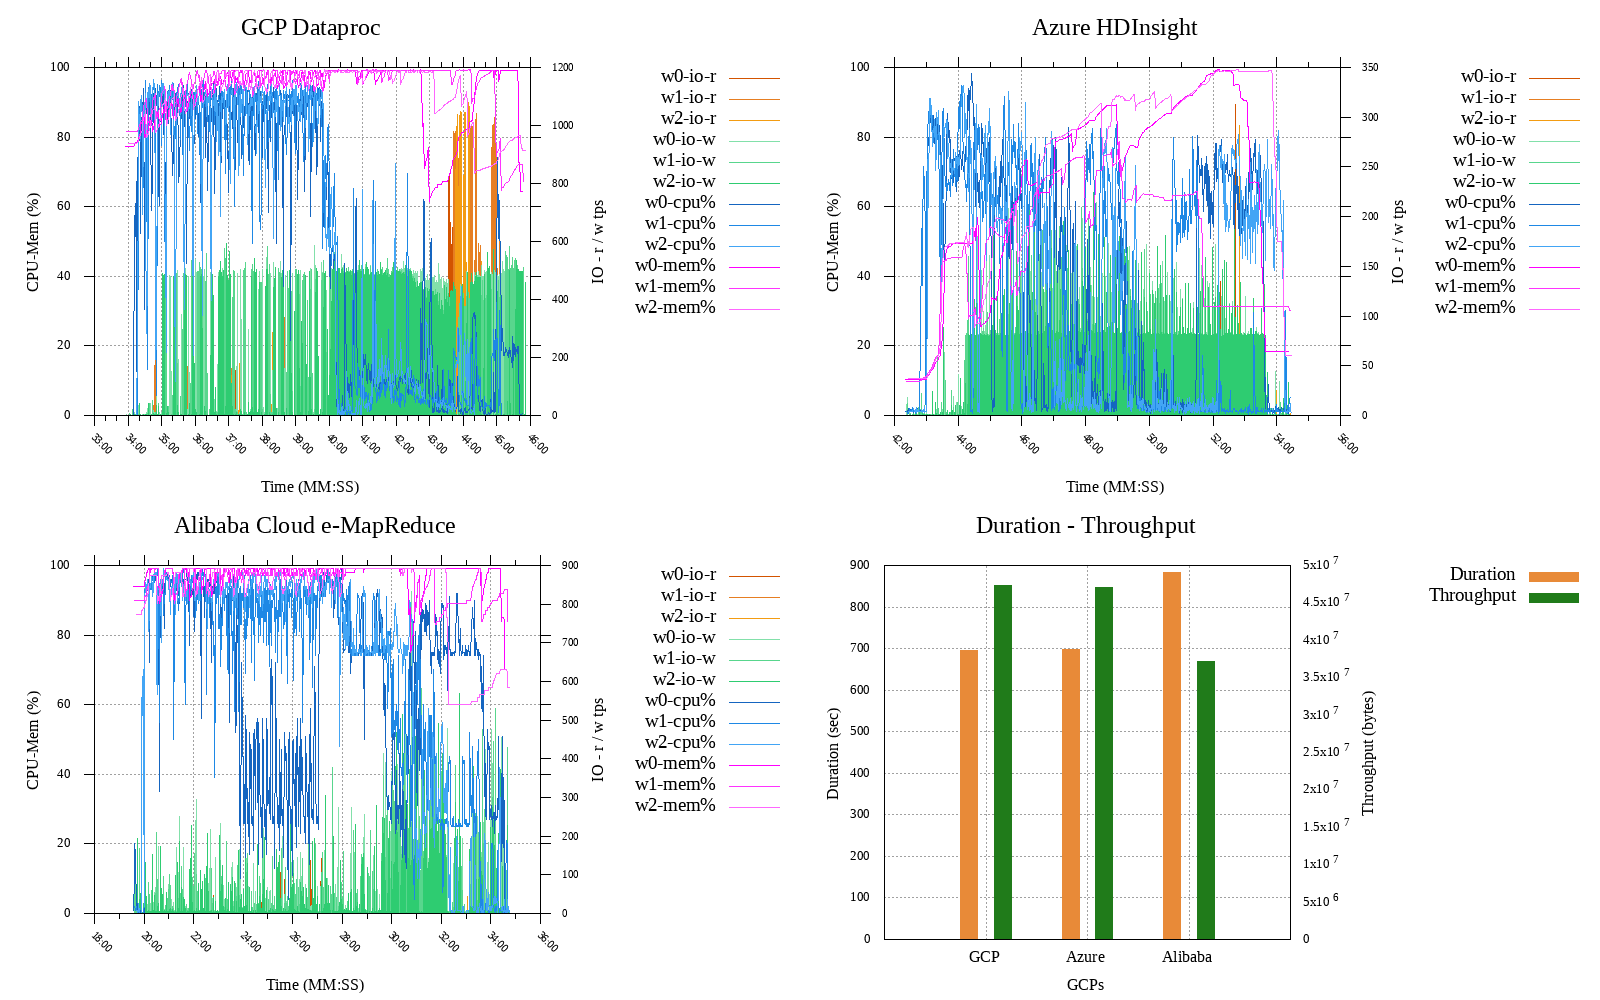
\includegraphics[width=\textwidth]{uc2-srt-g-cmidt}
%	\centering
%\end{figure}

Wordcount results in scale

%\begin{figure}[b]
%	\caption{UC2 - Wordcount (Tiny; 32 KB)}
%	\label{fig:uc2-wrdcnt-t-cmidt}
%	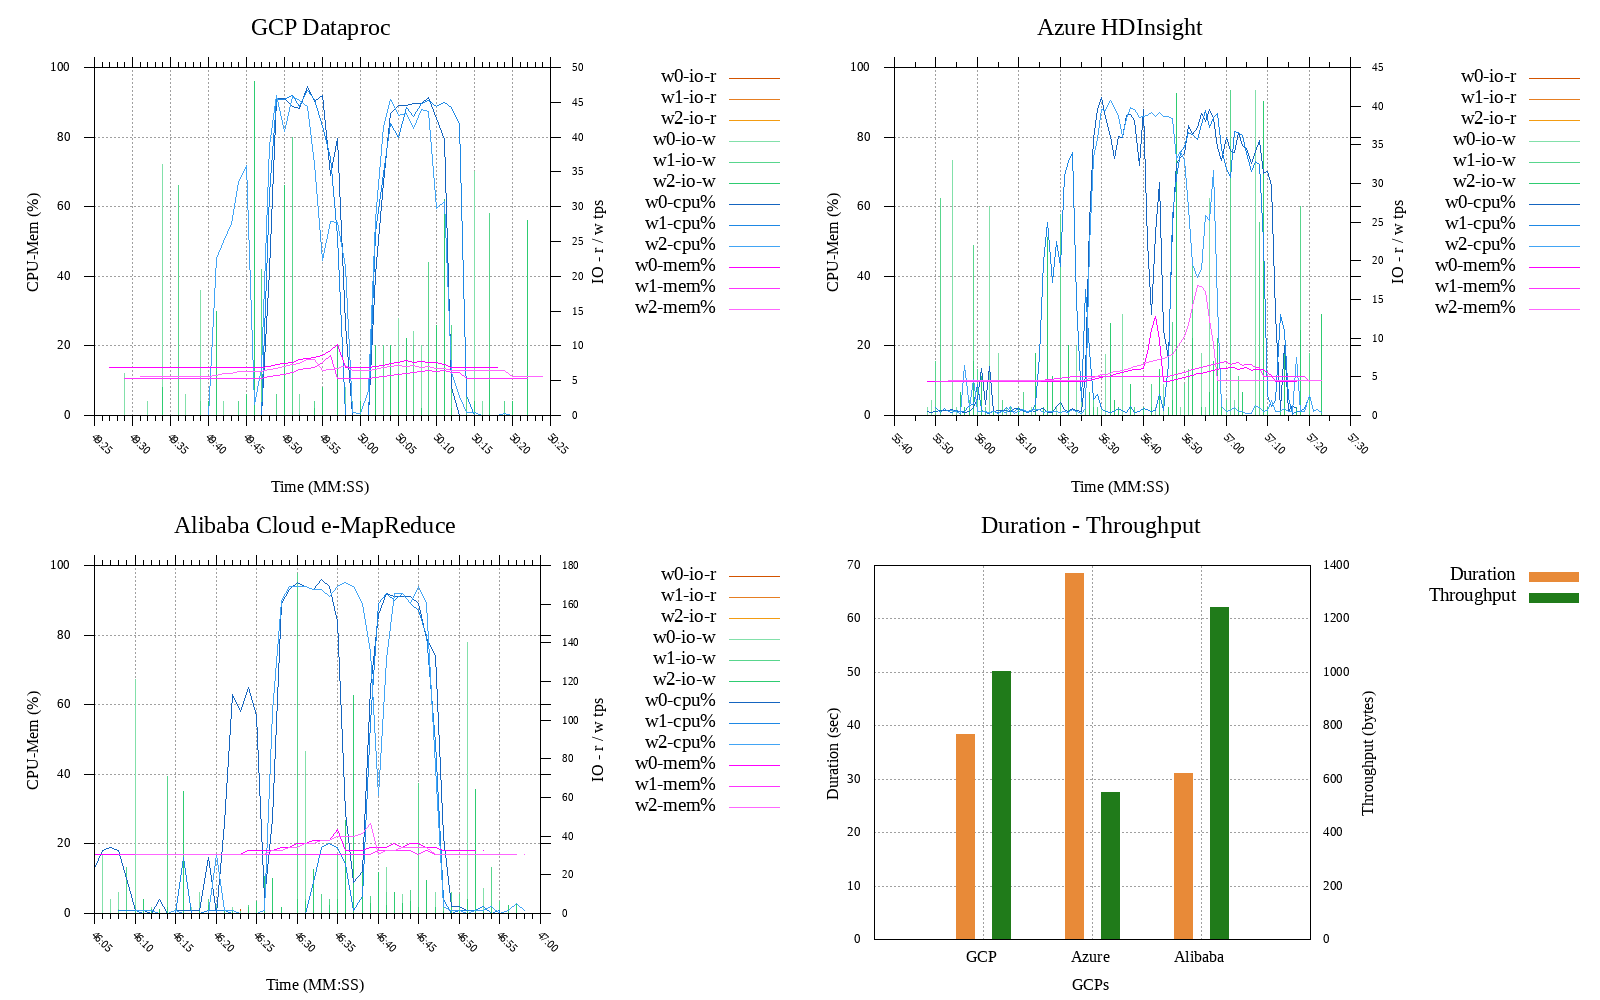
\includegraphics[width=\textwidth]{uc2-wrdcnt-t-cmidt}
%	\centering
%\end{figure}
%
%\begin{figure}[b]
%	\caption{UC2 - Wordcount (Small; 320 MB)}
%	\label{fig:uc2-wrdcnt-s-cmidt}
%	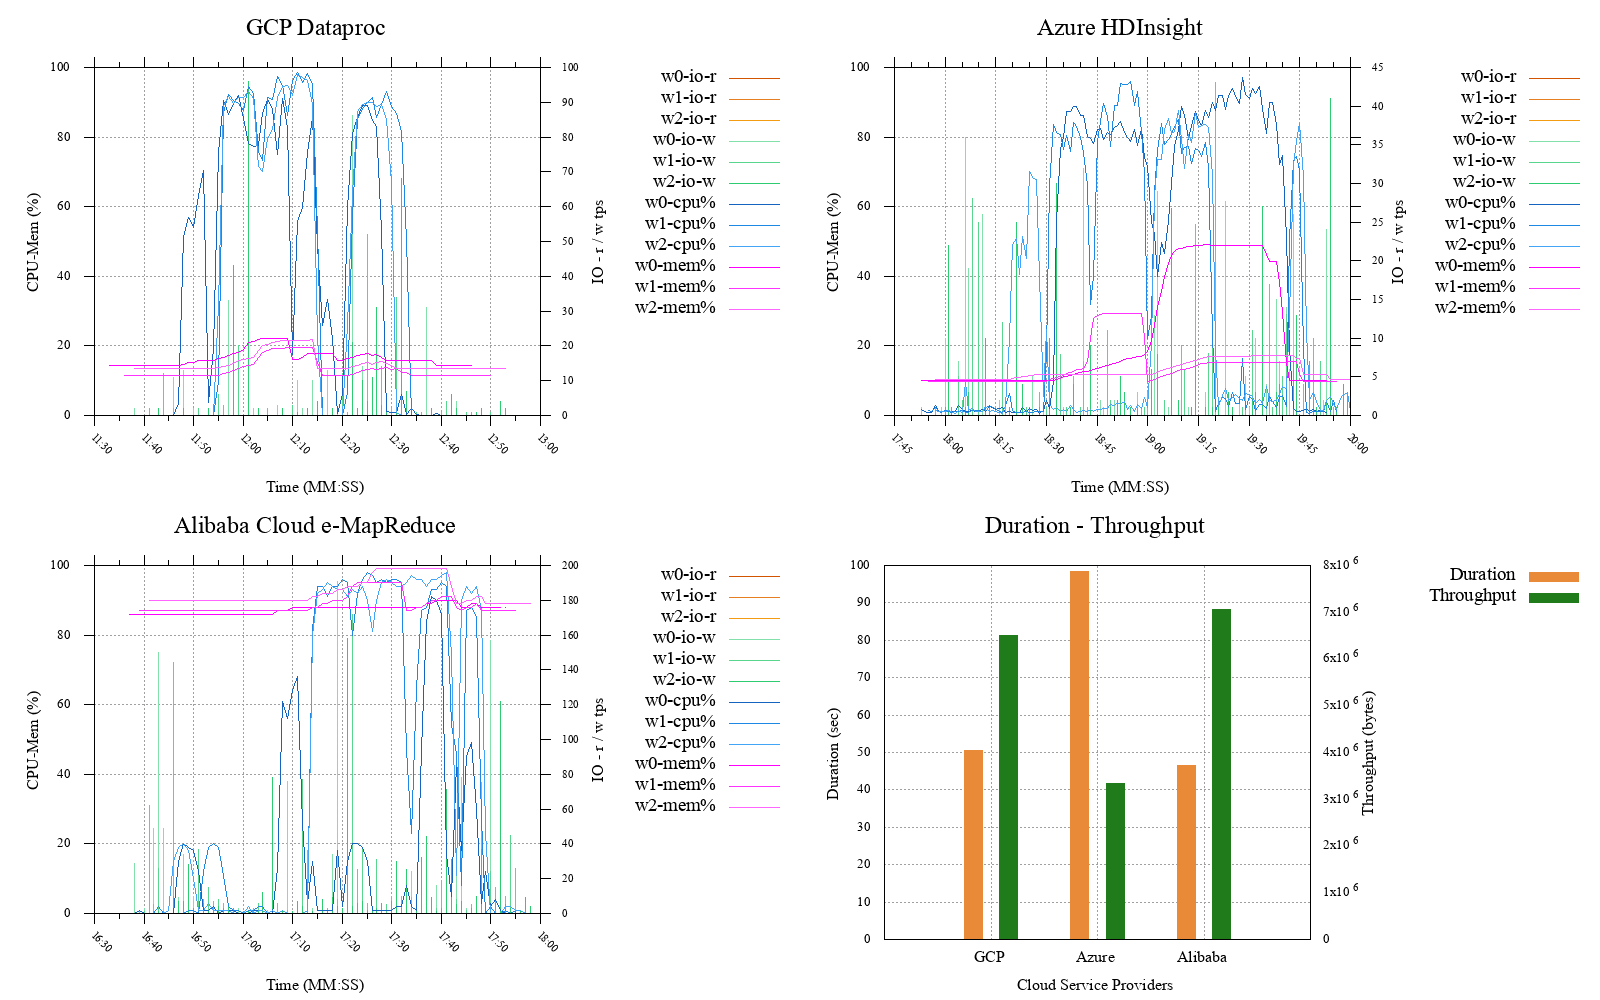
\includegraphics[width=\textwidth]{uc2-wrdcnt-s-cmidt}
%	\centering
%\end{figure}
%
%\begin{figure}[b]
%	\caption{UC2 - Wordcount (Large; 3.2 GB)}
%	\label{fig:uc2-wrdcnt-l-cmidt}
%	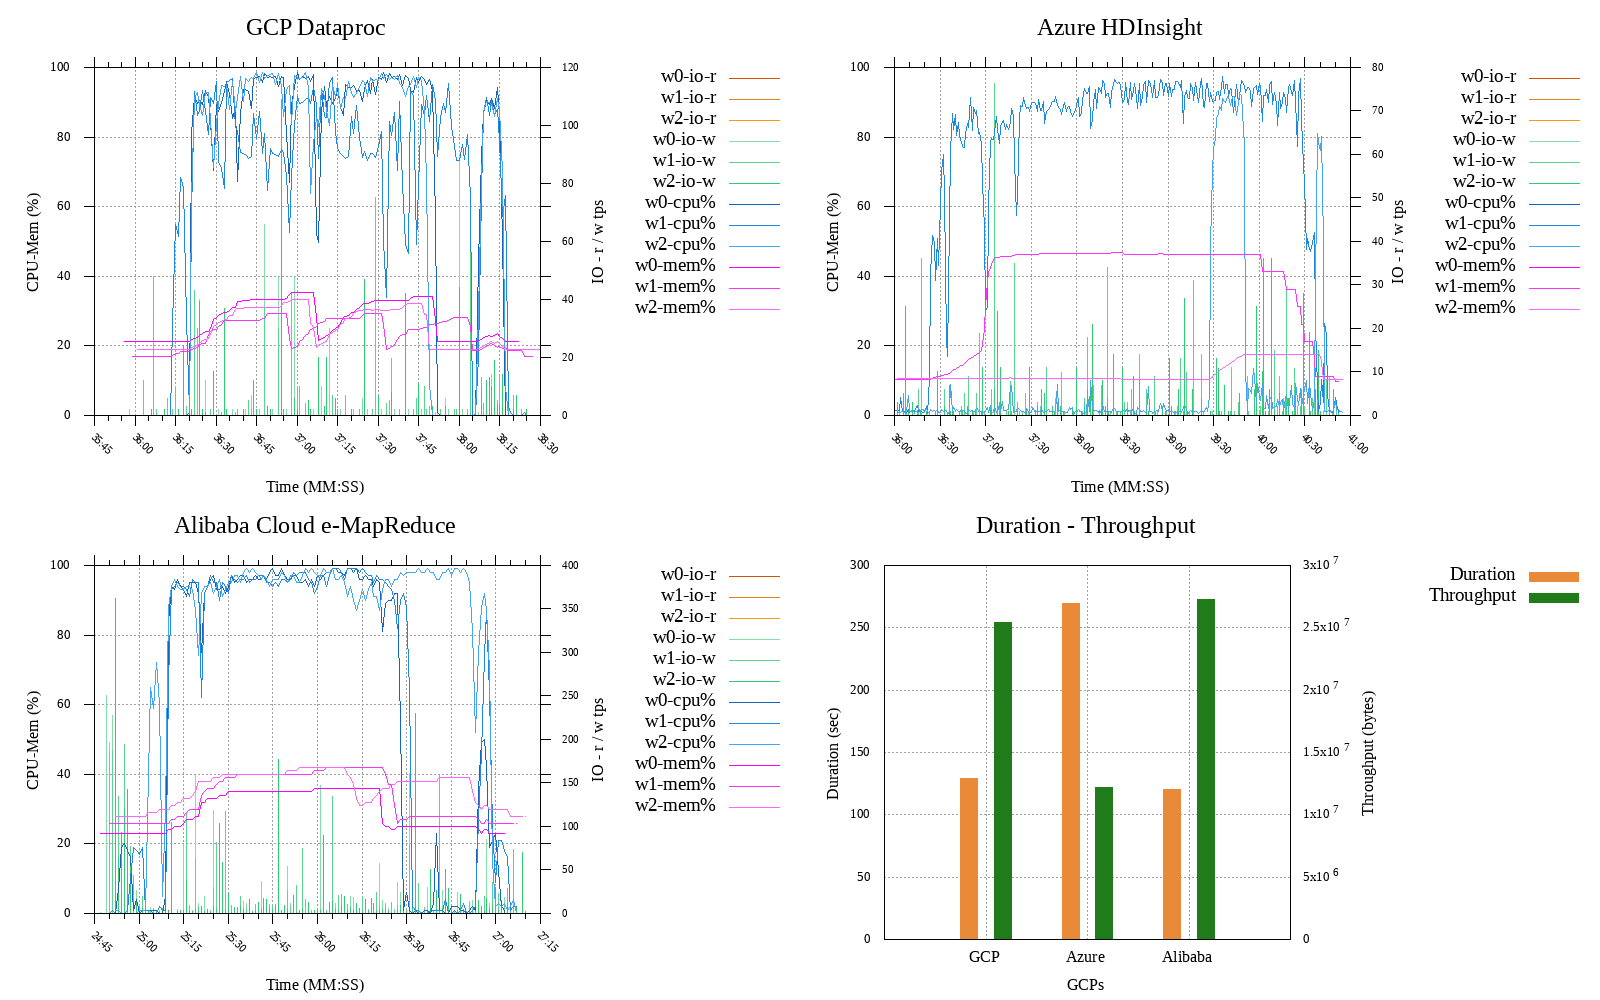
\includegraphics[width=\textwidth]{uc2-wrdcnt-l-cmidt}
%	\centering
%\end{figure}
%
%\begin{figure}[b]
%	\caption{UC2 - Wordcount (Huge; 32 GB)}
%	\label{fig:uc2-wrdcnt-h-cmidt}
%	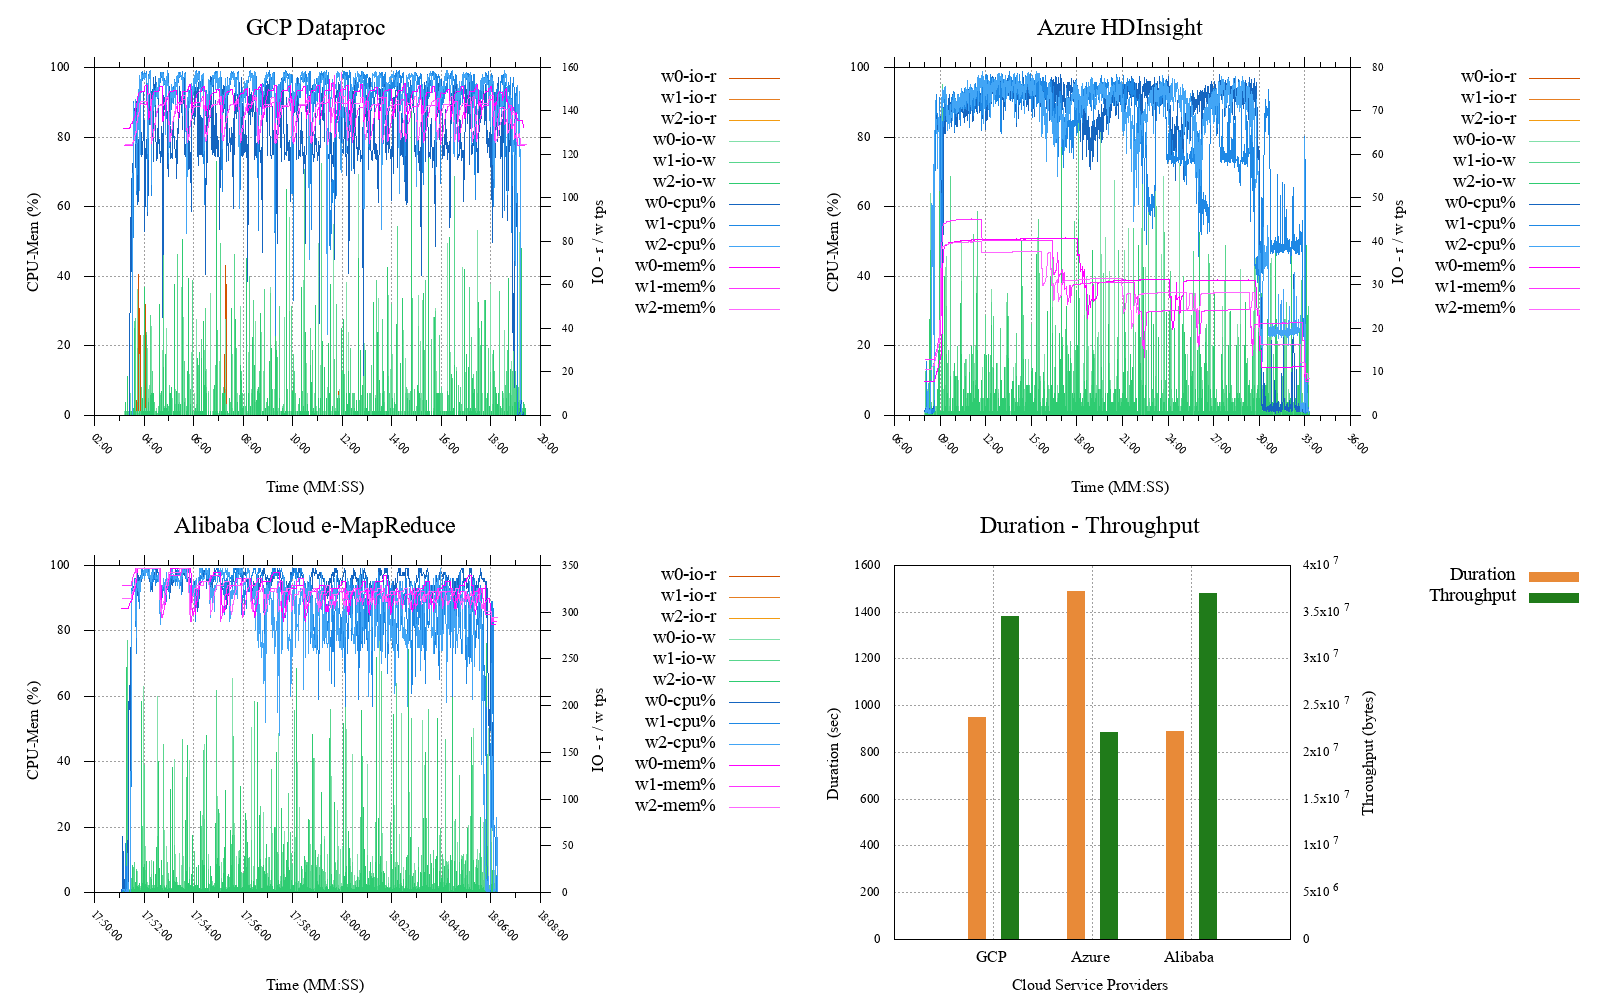
\includegraphics[width=\textwidth]{uc2-wrdcnt-h-cmidt}
%	\centering
%\end{figure}
%
%\begin{figure}[b]
%	\caption{UC2 - Wordcount (Gigantic; 320 GB)}
%	\label{fig:uc2-wrdcnt-g-cmidt}
%	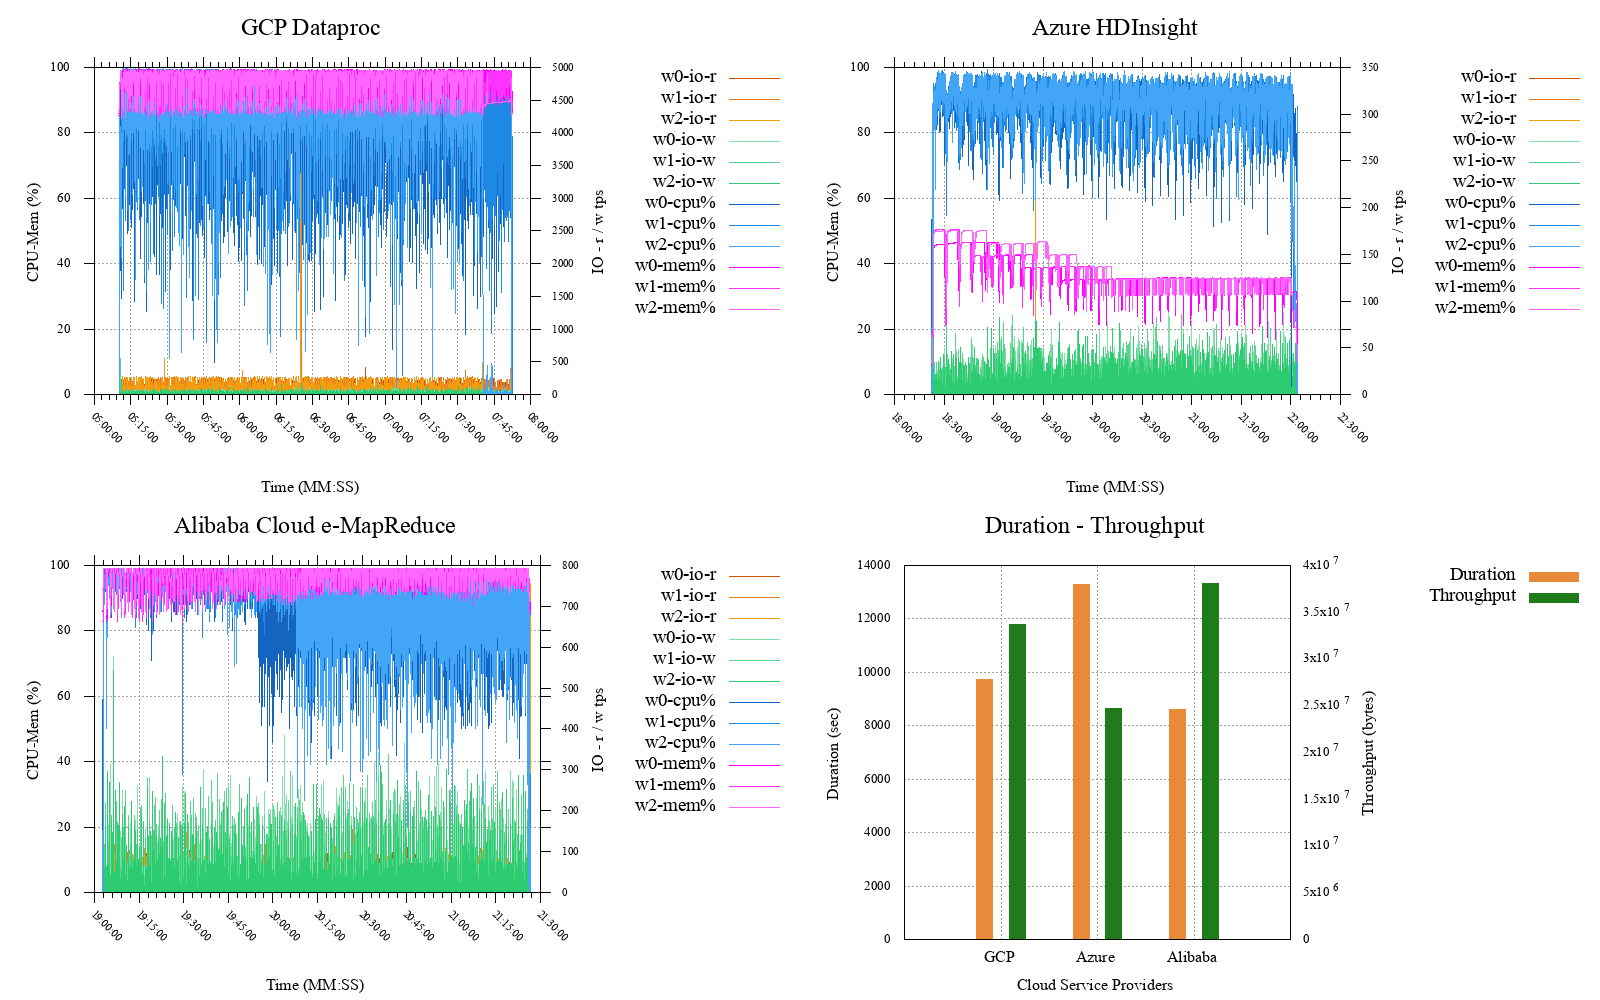
\includegraphics[width=\textwidth]{uc2-wrdcnt-g-cmidt}
%	\centering
%\end{figure}



\section{Discussion}
\paragraph{Limitations, workarounds, failures}One major limitation of this study has been the high-cost of benchmark executions' total running time which is charged in a pay-per-use manner leading the conductors halting benchmarks at only one successful execution for each workload. This is not fitting the best practise, though, where a benchmark would be executed thrice for each workload and the average performance results were taken. Following the best practise would have provided more stable outcomes especially in cases where there occurs very tiny difference between successive performances of respective providers. Hence, we recommend this study to be understood in terms of an attempt trying to bring more clarity to black-box natured managed Hadoop proposals' performance behavior by means of resource utilization dynamics, and as the managed services come out of the box without applying any performance tweaking configurations. We do not recommend this study to be understood as a grading board for the business values provided by respective CSPs.

HiBench comes with dependencies downloaded during its compilation process by Apache Maven. The Hive engine is one of those dependencies leveraged by HiBench for running SQL workloads Scan, Join, and Aggregation. Alibaba's e-Mapreduce comprises a ready made Hive hook trigerring a Java file to run post executional transactions for other services within the package. However this preconfiguration prevented HiBench from starting with respective benchmarks' execution since the HiBench based Hive engine does not include the aforementioned jar file defined for e-MapReduce's specific environment. Disabling the predefined Hive hook from Alibaba e-MapReduce's UI management console apparently solved this issue and enabled HiBench's SQL workloads to run, but the impact of this modification on the respective performance values remains unknown, hence the need to annotate it here. With GCP and Azure issues of this kind did not occur.

In Azure environment the Terasort benchmark running in data scale gigantic failed to complete in all three attempts we conducted where about 20\% of maps were completed. As distinct from GCP and Alibaba where the end user is liberate to chose HDFS or respective providers storage system as the cluster's file system, Azure obligates the user to go with WASB file system among other Azure storage services with a promise to Peta-scale. However, after inspecting the failure it turned out that the exception is not due the WASB file system. Even though WASB is predefined as the cluster's file system, during the application's run time YARN still leverages the cluster's HDFS file system for storing intermediary results failing to allocate free space on HDFS reaching specific levels of maps operators. The conductors marked this failure as a structural bottleneck, since all end users running Terasort operation at this scale would face the same error, and since resource utilization can be tracked up to the failure point and after, we kept this benchmark as disqualified.



\section{Conclusion}


\section{Bibliography styles}

There are various bibliography styles available. You can select the style of your choice in the preamble of this document. These styles are Elsevier styles based on standard styles like Harvard and Vancouver. Please use Bib\TeX\ to generate your bibliography and include DOIs whenever available.

Here are two sample references: \cite{Feynman1963118,Dirac1953888}.

\bibliography{mybibfile}

\end{document}